% Options for packages loaded elsewhere
\PassOptionsToPackage{unicode}{hyperref}
\PassOptionsToPackage{hyphens}{url}
\PassOptionsToPackage{dvipsnames,svgnames,x11names}{xcolor}
%
\documentclass[
  letterpaper,
  DIV=11,
  numbers=noendperiod]{scrreprt}

\usepackage{amsmath,amssymb}
\usepackage{iftex}
\ifPDFTeX
  \usepackage[T1]{fontenc}
  \usepackage[utf8]{inputenc}
  \usepackage{textcomp} % provide euro and other symbols
\else % if luatex or xetex
  \usepackage{unicode-math}
  \defaultfontfeatures{Scale=MatchLowercase}
  \defaultfontfeatures[\rmfamily]{Ligatures=TeX,Scale=1}
\fi
\usepackage{lmodern}
\ifPDFTeX\else  
    % xetex/luatex font selection
\fi
% Use upquote if available, for straight quotes in verbatim environments
\IfFileExists{upquote.sty}{\usepackage{upquote}}{}
\IfFileExists{microtype.sty}{% use microtype if available
  \usepackage[]{microtype}
  \UseMicrotypeSet[protrusion]{basicmath} % disable protrusion for tt fonts
}{}
\makeatletter
\@ifundefined{KOMAClassName}{% if non-KOMA class
  \IfFileExists{parskip.sty}{%
    \usepackage{parskip}
  }{% else
    \setlength{\parindent}{0pt}
    \setlength{\parskip}{6pt plus 2pt minus 1pt}}
}{% if KOMA class
  \KOMAoptions{parskip=half}}
\makeatother
\usepackage{xcolor}
\setlength{\emergencystretch}{3em} % prevent overfull lines
\setcounter{secnumdepth}{1}
% Make \paragraph and \subparagraph free-standing
\makeatletter
\ifx\paragraph\undefined\else
  \let\oldparagraph\paragraph
  \renewcommand{\paragraph}{
    \@ifstar
      \xxxParagraphStar
      \xxxParagraphNoStar
  }
  \newcommand{\xxxParagraphStar}[1]{\oldparagraph*{#1}\mbox{}}
  \newcommand{\xxxParagraphNoStar}[1]{\oldparagraph{#1}\mbox{}}
\fi
\ifx\subparagraph\undefined\else
  \let\oldsubparagraph\subparagraph
  \renewcommand{\subparagraph}{
    \@ifstar
      \xxxSubParagraphStar
      \xxxSubParagraphNoStar
  }
  \newcommand{\xxxSubParagraphStar}[1]{\oldsubparagraph*{#1}\mbox{}}
  \newcommand{\xxxSubParagraphNoStar}[1]{\oldsubparagraph{#1}\mbox{}}
\fi
\makeatother

\usepackage{color}
\usepackage{fancyvrb}
\newcommand{\VerbBar}{|}
\newcommand{\VERB}{\Verb[commandchars=\\\{\}]}
\DefineVerbatimEnvironment{Highlighting}{Verbatim}{commandchars=\\\{\}}
% Add ',fontsize=\small' for more characters per line
\usepackage{framed}
\definecolor{shadecolor}{RGB}{241,243,245}
\newenvironment{Shaded}{\begin{snugshade}}{\end{snugshade}}
\newcommand{\AlertTok}[1]{\textcolor[rgb]{0.68,0.00,0.00}{#1}}
\newcommand{\AnnotationTok}[1]{\textcolor[rgb]{0.37,0.37,0.37}{#1}}
\newcommand{\AttributeTok}[1]{\textcolor[rgb]{0.40,0.45,0.13}{#1}}
\newcommand{\BaseNTok}[1]{\textcolor[rgb]{0.68,0.00,0.00}{#1}}
\newcommand{\BuiltInTok}[1]{\textcolor[rgb]{0.00,0.23,0.31}{#1}}
\newcommand{\CharTok}[1]{\textcolor[rgb]{0.13,0.47,0.30}{#1}}
\newcommand{\CommentTok}[1]{\textcolor[rgb]{0.37,0.37,0.37}{#1}}
\newcommand{\CommentVarTok}[1]{\textcolor[rgb]{0.37,0.37,0.37}{\textit{#1}}}
\newcommand{\ConstantTok}[1]{\textcolor[rgb]{0.56,0.35,0.01}{#1}}
\newcommand{\ControlFlowTok}[1]{\textcolor[rgb]{0.00,0.23,0.31}{\textbf{#1}}}
\newcommand{\DataTypeTok}[1]{\textcolor[rgb]{0.68,0.00,0.00}{#1}}
\newcommand{\DecValTok}[1]{\textcolor[rgb]{0.68,0.00,0.00}{#1}}
\newcommand{\DocumentationTok}[1]{\textcolor[rgb]{0.37,0.37,0.37}{\textit{#1}}}
\newcommand{\ErrorTok}[1]{\textcolor[rgb]{0.68,0.00,0.00}{#1}}
\newcommand{\ExtensionTok}[1]{\textcolor[rgb]{0.00,0.23,0.31}{#1}}
\newcommand{\FloatTok}[1]{\textcolor[rgb]{0.68,0.00,0.00}{#1}}
\newcommand{\FunctionTok}[1]{\textcolor[rgb]{0.28,0.35,0.67}{#1}}
\newcommand{\ImportTok}[1]{\textcolor[rgb]{0.00,0.46,0.62}{#1}}
\newcommand{\InformationTok}[1]{\textcolor[rgb]{0.37,0.37,0.37}{#1}}
\newcommand{\KeywordTok}[1]{\textcolor[rgb]{0.00,0.23,0.31}{\textbf{#1}}}
\newcommand{\NormalTok}[1]{\textcolor[rgb]{0.00,0.23,0.31}{#1}}
\newcommand{\OperatorTok}[1]{\textcolor[rgb]{0.37,0.37,0.37}{#1}}
\newcommand{\OtherTok}[1]{\textcolor[rgb]{0.00,0.23,0.31}{#1}}
\newcommand{\PreprocessorTok}[1]{\textcolor[rgb]{0.68,0.00,0.00}{#1}}
\newcommand{\RegionMarkerTok}[1]{\textcolor[rgb]{0.00,0.23,0.31}{#1}}
\newcommand{\SpecialCharTok}[1]{\textcolor[rgb]{0.37,0.37,0.37}{#1}}
\newcommand{\SpecialStringTok}[1]{\textcolor[rgb]{0.13,0.47,0.30}{#1}}
\newcommand{\StringTok}[1]{\textcolor[rgb]{0.13,0.47,0.30}{#1}}
\newcommand{\VariableTok}[1]{\textcolor[rgb]{0.07,0.07,0.07}{#1}}
\newcommand{\VerbatimStringTok}[1]{\textcolor[rgb]{0.13,0.47,0.30}{#1}}
\newcommand{\WarningTok}[1]{\textcolor[rgb]{0.37,0.37,0.37}{\textit{#1}}}

\providecommand{\tightlist}{%
  \setlength{\itemsep}{0pt}\setlength{\parskip}{0pt}}\usepackage{longtable,booktabs,array}
\usepackage{calc} % for calculating minipage widths
% Correct order of tables after \paragraph or \subparagraph
\usepackage{etoolbox}
\makeatletter
\patchcmd\longtable{\par}{\if@noskipsec\mbox{}\fi\par}{}{}
\makeatother
% Allow footnotes in longtable head/foot
\IfFileExists{footnotehyper.sty}{\usepackage{footnotehyper}}{\usepackage{footnote}}
\makesavenoteenv{longtable}
\usepackage{graphicx}
\makeatletter
\newsavebox\pandoc@box
\newcommand*\pandocbounded[1]{% scales image to fit in text height/width
  \sbox\pandoc@box{#1}%
  \Gscale@div\@tempa{\textheight}{\dimexpr\ht\pandoc@box+\dp\pandoc@box\relax}%
  \Gscale@div\@tempb{\linewidth}{\wd\pandoc@box}%
  \ifdim\@tempb\p@<\@tempa\p@\let\@tempa\@tempb\fi% select the smaller of both
  \ifdim\@tempa\p@<\p@\scalebox{\@tempa}{\usebox\pandoc@box}%
  \else\usebox{\pandoc@box}%
  \fi%
}
% Set default figure placement to htbp
\def\fps@figure{htbp}
\makeatother
% definitions for citeproc citations
\NewDocumentCommand\citeproctext{}{}
\NewDocumentCommand\citeproc{mm}{%
  \begingroup\def\citeproctext{#2}\cite{#1}\endgroup}
\makeatletter
 % allow citations to break across lines
 \let\@cite@ofmt\@firstofone
 % avoid brackets around text for \cite:
 \def\@biblabel#1{}
 \def\@cite#1#2{{#1\if@tempswa , #2\fi}}
\makeatother
\newlength{\cslhangindent}
\setlength{\cslhangindent}{1.5em}
\newlength{\csllabelwidth}
\setlength{\csllabelwidth}{3em}
\newenvironment{CSLReferences}[2] % #1 hanging-indent, #2 entry-spacing
 {\begin{list}{}{%
  \setlength{\itemindent}{0pt}
  \setlength{\leftmargin}{0pt}
  \setlength{\parsep}{0pt}
  % turn on hanging indent if param 1 is 1
  \ifodd #1
   \setlength{\leftmargin}{\cslhangindent}
   \setlength{\itemindent}{-1\cslhangindent}
  \fi
  % set entry spacing
  \setlength{\itemsep}{#2\baselineskip}}}
 {\end{list}}
\usepackage{calc}
\newcommand{\CSLBlock}[1]{\hfill\break\parbox[t]{\linewidth}{\strut\ignorespaces#1\strut}}
\newcommand{\CSLLeftMargin}[1]{\parbox[t]{\csllabelwidth}{\strut#1\strut}}
\newcommand{\CSLRightInline}[1]{\parbox[t]{\linewidth - \csllabelwidth}{\strut#1\strut}}
\newcommand{\CSLIndent}[1]{\hspace{\cslhangindent}#1}

\KOMAoption{captions}{tablesignature}
\makeatletter
\@ifpackageloaded{tcolorbox}{}{\usepackage[skins,breakable]{tcolorbox}}
\@ifpackageloaded{fontawesome5}{}{\usepackage{fontawesome5}}
\definecolor{quarto-callout-color}{HTML}{909090}
\definecolor{quarto-callout-note-color}{HTML}{0758E5}
\definecolor{quarto-callout-important-color}{HTML}{CC1914}
\definecolor{quarto-callout-warning-color}{HTML}{EB9113}
\definecolor{quarto-callout-tip-color}{HTML}{00A047}
\definecolor{quarto-callout-caution-color}{HTML}{FC5300}
\definecolor{quarto-callout-color-frame}{HTML}{acacac}
\definecolor{quarto-callout-note-color-frame}{HTML}{4582ec}
\definecolor{quarto-callout-important-color-frame}{HTML}{d9534f}
\definecolor{quarto-callout-warning-color-frame}{HTML}{f0ad4e}
\definecolor{quarto-callout-tip-color-frame}{HTML}{02b875}
\definecolor{quarto-callout-caution-color-frame}{HTML}{fd7e14}
\makeatother
\makeatletter
\@ifpackageloaded{bookmark}{}{\usepackage{bookmark}}
\makeatother
\makeatletter
\@ifpackageloaded{caption}{}{\usepackage{caption}}
\AtBeginDocument{%
\ifdefined\contentsname
  \renewcommand*\contentsname{Table of contents}
\else
  \newcommand\contentsname{Table of contents}
\fi
\ifdefined\listfigurename
  \renewcommand*\listfigurename{List of Figures}
\else
  \newcommand\listfigurename{List of Figures}
\fi
\ifdefined\listtablename
  \renewcommand*\listtablename{List of Tables}
\else
  \newcommand\listtablename{List of Tables}
\fi
\ifdefined\figurename
  \renewcommand*\figurename{Fig.}
\else
  \newcommand\figurename{Fig.}
\fi
\ifdefined\tablename
  \renewcommand*\tablename{Tab.}
\else
  \newcommand\tablename{Tab.}
\fi
}
\@ifpackageloaded{float}{}{\usepackage{float}}
\floatstyle{ruled}
\@ifundefined{c@chapter}{\newfloat{codelisting}{h}{lop}}{\newfloat{codelisting}{h}{lop}[chapter]}
\floatname{codelisting}{Listing}
\newcommand*\listoflistings{\listof{codelisting}{List of Listings}}
\makeatother
\makeatletter
\makeatother
\makeatletter
\@ifpackageloaded{caption}{}{\usepackage{caption}}
\@ifpackageloaded{subcaption}{}{\usepackage{subcaption}}
\makeatother

\usepackage{bookmark}

\IfFileExists{xurl.sty}{\usepackage{xurl}}{} % add URL line breaks if available
\urlstyle{same} % disable monospaced font for URLs
\hypersetup{
  pdftitle={Echoes},
  pdfauthor={Jean-François Barthélémy},
  colorlinks=true,
  linkcolor={blue},
  filecolor={Maroon},
  citecolor={Blue},
  urlcolor={Blue},
  pdfcreator={LaTeX via pandoc}}


\title{Echoes}
\usepackage{etoolbox}
\makeatletter
\providecommand{\subtitle}[1]{% add subtitle to \maketitle
  \apptocmd{\@title}{\par {\large #1 \par}}{}{}
}
\makeatother
\subtitle{Extended Calculator of HOmogEnization Schemes}
\author{Jean-François Barthélémy}
\date{2025-01-24}

\begin{document}
\maketitle

\renewcommand*\contentsname{Table of contents}
{
\hypersetup{linkcolor=}
\setcounter{tocdepth}{2}
\tableofcontents
}

\bookmarksetup{startatroot}

\chapter*{Welcome}\label{sec-welcome}
\addcontentsline{toc}{chapter}{Welcome}

\markboth{Welcome}{Welcome}

\begin{center}
\includegraphics[width=0.2\linewidth,height=\textheight,keepaspectratio]{img/cover.pdf}
\end{center}

The library \texttt{echoes} allows to implement various mean-field
homogenization schemes of random media involving different types of
heterogeneities in the framework of elasticity, conductivity,
viscoelasticity as well as nonlinear homogenization.

This book gathers tutorials presenting the main features of the library:

\begin{itemize}
\tightlist
\item
  elements of tensor calculus,
\item
  Hill and Eshelby tensors and their derivatives with respect to
  reference medium moduli,
\item
  concentration problems,
\item
  RVEs and schemes in linear homogenization,
\item
  extension to nonlinear homogenization,
\item
  extension to linear time-dependent behaviors.
\end{itemize}

\section*{Download}\label{download}
\addcontentsline{toc}{section}{Download}

\markright{Download}

The core of \texttt{echoes} has been developed in C++ and wrapped by a
Python interface. Hence its use requires first the installation of a
Python environment including \texttt{pip} executable (for instance
\href{https://www.anaconda.com/products/distribution}{Anaconda}).

Wheel packages can be downloaded for various versions of Python under
Windows or Linux by choosing the appropriate file for your configuration
under the link

https://doi.org/10.5281/zenodo.10559657

Once in possession of the relevant \texttt{.whl} file, the package can
be installed in a console (Anaconda console or any console allowing to
run \texttt{pip}) by

\begin{Shaded}
\begin{Highlighting}[]
\NormalTok{pip install }\OperatorTok{{-}}\NormalTok{U echoes}\OperatorTok{{-}}\NormalTok{XYZ.whl}
\CommentTok{\# replacing echoes{-}XYZ.whl by the correct path to the whl file}
\end{Highlighting}
\end{Shaded}

\section*{Citation}\label{citation}
\addcontentsline{toc}{section}{Citation}

\markright{Citation}

If you use \texttt{echoes}, please cite it as
(\citeproc{ref-echoes}{Barthélémy, 2022}) or in \texttt{bibtex} style

\begin{Shaded}
\begin{Highlighting}[]
\NormalTok{@software\{echoes,}
\NormalTok{  title = \{Echoes: \{\{Extended Calculator\}\} of \{\{HOmogEnization Schemes\}\}\},}
\NormalTok{  shorttitle = \{Echoes\},}
\NormalTok{  author = \{Barthélémy, Jean{-}François\},}
\NormalTok{  date = \{2022{-}11{-}22\},}
\NormalTok{  doi = \{10.5281/ZENODO.10559657\},}
\NormalTok{  url = \{https://zenodo.org/record/10559657\},}
\NormalTok{  organization = \{Zenodo\},}
\NormalTok{  version = \{v1.0.0\},}
\NormalTok{\}}
\end{Highlighting}
\end{Shaded}

All this work is licensed under the
\href{https://creativecommons.org/licenses/by-sa/4.0/}{Creative Commons
Attribution-ShareAlike 4.0 International License}
\pandocbounded{\includegraphics[keepaspectratio]{index_files/mediabag/88x31.png}}.

\section*{About the author}\label{about-the-author}
\addcontentsline{toc}{section}{About the author}

\markright{About the author}

Jean-François Barthélémy is a researcher at
\href{https://www.cerema.fr/en}{Cerema} in the research team
\href{https://www.cerema.fr/fr/presse/dossier\%20cerema-universite-gustave-eiffel-creent-unite-mixte}{UMR
MCD}.

\begin{itemize}
\item
  \href{https://github.com/jfbarthelemy}{GitHub}
\item

  \href{https://www.researchgate.net/profile/Jean-Francois_Barthelemy}{ResearchGate}
\item

  \href{https://scholar.google.com/citations?user=RVjtCiAAAAAJ&hl=en}{Google
  scholar}
\item
  📚
  \href{https://hal.archives-ouvertes.fr/search/index/?q=\%2A&authIdHal_s=jfbarthelemy}{HAL}
\item
  🌍 \href{https://www.webofscience.com/wos/author/record/449919}{Web Of
  Science}
\item
  \href{https://orcid.org/0000-0002-1968-8939}{ORCID}
\item
  📩 \href{mailto:jf.barthelemy@cerema.fr}{Email}
\end{itemize}

\begin{center}\rule{0.5\linewidth}{0.5pt}\end{center}

Powered by \href{https://quarto.org/}{Quarto}.

\(\,\)

\bookmarksetup{startatroot}

\chapter*{Introduction}\label{sec-intro}
\addcontentsline{toc}{chapter}{Introduction}

\markboth{Introduction}{Introduction}

This book is aimed at researchers, engineers and students, knowing the
fundamentals of mean-field theory to help them learn how to use the
\texttt{echoes} library with some brief theoretical recalls when
relevant. For a more exhaustive presentation of the theory of random
medium homogenization, see (\citeproc{ref-bornert2001a}{Bornert et al.,
2001}), (\citeproc{ref-milton2002}{Milton, 2002}),
(\citeproc{ref-torquato2002}{Torquato, 2002}) or
(\citeproc{ref-kachanov2018}{Kachanov and Sevostianov, 2018}) among
others.

The objectives of the library can be summarized as follows:

\begin{itemize}
\item
  simple and quick implementation of Eshelby problems and homogenization
  schemes,
\item
  multi-physics and multi-scale homogenization,
\item
  effects of microstructure changes by chemical, physical or mechanical
  process.
\end{itemize}

\begin{tcolorbox}[enhanced jigsaw, left=2mm, bottomrule=.15mm, colbacktitle=quarto-callout-note-color!10!white, colback=white, colframe=quarto-callout-note-color-frame, rightrule=.15mm, bottomtitle=1mm, toptitle=1mm, titlerule=0mm, title={Features}, toprule=.15mm, arc=.35mm, opacityback=0, opacitybacktitle=0.6, leftrule=.75mm, breakable, coltitle=black]

\begin{itemize}
\item
  Eshelby problem solved at 2nd (conductivity) et 4th orders
  (elasticity)
\item
  Isotropy and anisotropy
\item
  Several types of inclusions including generic (user-defined) inclusion
\item
  Large variety of schemes
\item
  Derivatives of the macroscopic elasticity with respect to lower scale
  moduli
\item
  Aging linear viscoelasticity
\item
  Complex moduli
\end{itemize}

\end{tcolorbox}

In this manual, some snippets of Python codes are presented. The
\texttt{echoes} library can be imported as

\begin{Shaded}
\begin{Highlighting}[]
\ImportTok{from}\NormalTok{ echoes }\ImportTok{import} \OperatorTok{*}
\end{Highlighting}
\end{Shaded}

or, to avoid any ambiguity between libraries, as

\begin{Shaded}
\begin{Highlighting}[]
\ImportTok{import}\NormalTok{ echoes }\ImportTok{as}\NormalTok{ ec}
\end{Highlighting}
\end{Shaded}

A usual start of any tutorial could be the following

\begin{Shaded}
\begin{Highlighting}[]
\ImportTok{import}\NormalTok{ numpy }\ImportTok{as}\NormalTok{ np}
\ImportTok{from}\NormalTok{ echoes }\ImportTok{import} \OperatorTok{*}
\ImportTok{import}\NormalTok{ matplotlib.pyplot }\ImportTok{as}\NormalTok{ plt }\CommentTok{\# if plots are needed}

\NormalTok{np.set\_printoptions(precision}\OperatorTok{=}\DecValTok{8}\NormalTok{, suppress}\OperatorTok{=}\VariableTok{True}\NormalTok{)}
\CommentTok{\# to display only 8 significant digits of array components}
\end{Highlighting}
\end{Shaded}

Whenever they are omitted, it is implicitly considered that these lines
have previously been added.

\(\,\)

\part{𝗘𝗹𝗲𝗺𝗲𝗻𝘁𝘀 𝗼𝗳 𝘁𝗲𝗻𝘀𝗼𝗿 𝗰𝗮𝗹𝗰𝘂𝗹𝘂𝘀}

\chapter{Kelvin-Mandel notation}\label{sec-kelvin_mandel}

\begin{tcolorbox}[enhanced jigsaw, left=2mm, bottomrule=.15mm, colbacktitle=quarto-callout-important-color!10!white, colback=white, colframe=quarto-callout-important-color-frame, rightrule=.15mm, bottomtitle=1mm, toptitle=1mm, titlerule=0mm, title={Objectives}, toprule=.15mm, arc=.35mm, opacityback=0, opacitybacktitle=0.6, leftrule=.75mm, breakable, coltitle=black]

Before introducing the specific objects of \texttt{echoes} devoted to
tensor calculations in isotropic or anisotropic contexts, this tutorial
aims at providing the syntax allowing to represent second-order or
fourth-order tensors under the form of matrices in the Kelvin-Mandel
notation as detailed in Section~\ref{sec-KM}.

\end{tcolorbox}

\begin{tcolorbox}[enhanced jigsaw, left=2mm, bottomrule=.15mm, colbacktitle=quarto-callout-note-color!10!white, colback=white, colframe=quarto-callout-note-color-frame, rightrule=.15mm, bottomtitle=1mm, toptitle=1mm, titlerule=0mm, title={Download}, toprule=.15mm, arc=.35mm, opacityback=0, opacitybacktitle=0.6, leftrule=.75mm, breakable, coltitle=black]

\begin{itemize}
\item
  \href{kelvin_mandel.py}{Python script}
\item
  \href{kelvin_mandel.ipynb}{Jupyter notebook}
\end{itemize}

\end{tcolorbox}

\begin{tcolorbox}[enhanced jigsaw, left=2mm, bottomrule=.15mm, colbacktitle=quarto-callout-tip-color!10!white, colback=white, colframe=quarto-callout-tip-color-frame, rightrule=.15mm, bottomtitle=1mm, toptitle=1mm, titlerule=0mm, title={Imports}, toprule=.15mm, arc=.35mm, opacityback=0, opacitybacktitle=0.6, leftrule=.75mm, breakable, coltitle=black]

\begin{Shaded}
\begin{Highlighting}[]
\ImportTok{import}\NormalTok{ numpy }\ImportTok{as}\NormalTok{ np}
\ImportTok{from}\NormalTok{ echoes }\ImportTok{import} \OperatorTok{*}
\ImportTok{import}\NormalTok{ math, random}

\NormalTok{np.set\_printoptions(precision}\OperatorTok{=}\DecValTok{8}\NormalTok{, suppress}\OperatorTok{=}\VariableTok{True}\NormalTok{)}
\CommentTok{\# to display only 8 significant digits of array components}
\end{Highlighting}
\end{Shaded}

\end{tcolorbox}

A symmetric \(3×3\) second-order matrix can be transformed in a vector
of \(\R^6\) by the function \texttt{KM} consistently with \ref{eq-KM2}.
The inverse is done by \texttt{invKM}.

\begin{Shaded}
\begin{Highlighting}[]
\NormalTok{α }\OperatorTok{=}\NormalTok{ np.random.rand(}\DecValTok{3}\NormalTok{, }\DecValTok{3}\NormalTok{) }\OperatorTok{;}\NormalTok{ ε }\OperatorTok{=}\NormalTok{ (α}\OperatorTok{+}\NormalTok{α.T)}\OperatorTok{/}\DecValTok{2}
\BuiltInTok{print}\NormalTok{(}\StringTok{"ε =}\CharTok{\textbackslash{}n}\StringTok{"}\NormalTok{,ε)}
\BuiltInTok{print}\NormalTok{(}\StringTok{"KM(ε) =}\CharTok{\textbackslash{}n}\StringTok{"}\NormalTok{,KM(ε))}
\ControlFlowTok{assert}\NormalTok{ np.allclose(invKM(KM(ε)), ε), }\StringTok{"error"}
\end{Highlighting}
\end{Shaded}

\begin{verbatim}
ε =
 [[0.11518697 0.36389157 0.68531149]
 [0.36389157 0.24973352 0.85029112]
 [0.68531149 0.85029112 0.36267488]]
KM(ε) =
 [0.11518697 0.24973352 0.36267488 1.20249323 0.9691768  0.5146204 ]
\end{verbatim}

Given a \(3×3×3×3\) array \texttt{c} (of type \texttt{numpy.ndarray})
satisfying major and minor symmetries (see Section~\ref{sec-KM}), the
corresponding \(6×6\) matrix \texttt{C} obtained by Kelvin-Mandel
transform is calculated by \texttt{C\ =\ KM(c)}. Conversely, if
\texttt{C} is a positive definite matrix, \texttt{c} is calculated by
\texttt{c\ =\ invKM(C)}.

\begin{Shaded}
\begin{Highlighting}[]
\NormalTok{A }\OperatorTok{=}\NormalTok{ np.random.rand(}\DecValTok{6}\NormalTok{,}\DecValTok{6}\NormalTok{)}
\NormalTok{C }\OperatorTok{=}\NormalTok{ A.T.dot(A) }\OperatorTok{+}\NormalTok{ np.eye(}\DecValTok{6}\NormalTok{) }\CommentTok{\# generation of an arbitrary positive definite matrix}
\NormalTok{c }\OperatorTok{=}\NormalTok{ invKM(C)}
\BuiltInTok{print}\NormalTok{(}\StringTok{"C =}\CharTok{\textbackslash{}n}\StringTok{"}\NormalTok{,C)}
\BuiltInTok{print}\NormalTok{(}\StringTok{"c =}\CharTok{\textbackslash{}n}\StringTok{"}\NormalTok{,c)}
\ControlFlowTok{assert}\NormalTok{ np.allclose(KM(c), C), }\StringTok{"error: KM(c) should be equal to C"}
\end{Highlighting}
\end{Shaded}

\begin{verbatim}
C =
 [[2.77299328 2.2444528  1.04322629 1.40082289 1.84329357 1.25925132]
 [2.2444528  4.43283651 1.60572381 1.59875001 2.60033506 2.04101056]
 [1.04322629 1.60572381 2.59112573 0.86867369 1.86259637 0.75512835]
 [1.40082289 1.59875001 0.86867369 2.31689298 1.55525077 0.87239494]
 [1.84329357 2.60033506 1.86259637 1.55525077 3.88870775 1.40974405]
 [1.25925132 2.04101056 0.75512835 0.87239494 1.40974405 2.32015014]]
c =
 [[[[2.77299328 0.89042515 1.30340538]
   [0.89042515 2.2444528  0.99053136]
   [1.30340538 0.99053136 1.04322629]]

  [[0.89042515 1.16007507 0.70487202]
   [1.16007507 1.44321241 0.43619747]
   [0.70487202 0.43619747 0.53395637]]

  [[1.30340538 0.70487202 1.94435387]
   [0.70487202 1.83871456 0.77762538]
   [1.94435387 0.77762538 1.31705452]]]


 [[[0.89042515 1.16007507 0.70487202]
   [1.16007507 1.44321241 0.43619747]
   [0.70487202 0.43619747 0.53395637]]

  [[2.2444528  1.44321241 1.83871456]
   [1.44321241 4.43283651 1.13048697]
   [1.83871456 1.13048697 1.60572381]]

  [[0.99053136 0.43619747 0.77762538]
   [0.43619747 1.13048697 1.15844649]
   [0.77762538 1.15844649 0.61424505]]]


 [[[1.30340538 0.70487202 1.94435387]
   [0.70487202 1.83871456 0.77762538]
   [1.94435387 0.77762538 1.31705452]]

  [[0.99053136 0.43619747 0.77762538]
   [0.43619747 1.13048697 1.15844649]
   [0.77762538 1.15844649 0.61424505]]

  [[1.04322629 0.53395637 1.31705452]
   [0.53395637 1.60572381 0.61424505]
   [1.31705452 0.61424505 2.59112573]]]]
\end{verbatim}

\(\,\)

\chapter{Rotation matrices}\label{sec-rot_tensors}

\begin{tcolorbox}[enhanced jigsaw, left=2mm, bottomrule=.15mm, colbacktitle=quarto-callout-important-color!10!white, colback=white, colframe=quarto-callout-important-color-frame, rightrule=.15mm, bottomtitle=1mm, toptitle=1mm, titlerule=0mm, title={Objectives}, toprule=.15mm, arc=.35mm, opacityback=0, opacitybacktitle=0.6, leftrule=.75mm, breakable, coltitle=black]

This tutorial presents the construction of rotation matrices in \(\R^3\)
in the convention proposed in Section~\ref{sec-rottens} for Euler
angles.

\end{tcolorbox}

\begin{tcolorbox}[enhanced jigsaw, left=2mm, bottomrule=.15mm, colbacktitle=quarto-callout-note-color!10!white, colback=white, colframe=quarto-callout-note-color-frame, rightrule=.15mm, bottomtitle=1mm, toptitle=1mm, titlerule=0mm, title={Download}, toprule=.15mm, arc=.35mm, opacityback=0, opacitybacktitle=0.6, leftrule=.75mm, breakable, coltitle=black]

\begin{itemize}
\item
  \href{rot_matrices.py}{Python script}
\item
  \href{rot_matrices.ipynb}{Jupyter notebook}
\end{itemize}

\end{tcolorbox}

\begin{tcolorbox}[enhanced jigsaw, left=2mm, bottomrule=.15mm, colbacktitle=quarto-callout-tip-color!10!white, colback=white, colframe=quarto-callout-tip-color-frame, rightrule=.15mm, bottomtitle=1mm, toptitle=1mm, titlerule=0mm, title={Imports}, toprule=.15mm, arc=.35mm, opacityback=0, opacitybacktitle=0.6, leftrule=.75mm, breakable, coltitle=black]

\begin{Shaded}
\begin{Highlighting}[]
\ImportTok{import}\NormalTok{ numpy }\ImportTok{as}\NormalTok{ np}
\ImportTok{from}\NormalTok{ echoes }\ImportTok{import} \OperatorTok{*}
\ImportTok{import}\NormalTok{ math, random}

\NormalTok{np.set\_printoptions(precision}\OperatorTok{=}\DecValTok{8}\NormalTok{, suppress}\OperatorTok{=}\VariableTok{True}\NormalTok{)}
\CommentTok{\# to display only 8 significant digits of array components}
\end{Highlighting}
\end{Shaded}

\end{tcolorbox}

Given the Euler angles \texttt{θ,\ ϕ,\ ψ} defined in
Section~\ref{sec-rottens} and more particularly in
Fig.~\ref{fig-eulerangles}, the rotation matrix (\ref{eq-rot3}) recalled
here \[
\small
\mat{R}=
   \left(
   \begin{array}{ccc}
   c_\theta  c_\psi  c_\phi - s_\psi  s_\phi & - c_\theta  c_\phi  s_\psi - c_\psi  s_\phi & c_\phi  s_\theta \\
   c_\theta  c_\psi  s_\phi + c_\phi  s_\psi & - c_\theta  s_\psi  s_\phi + c_\psi  c_\phi & s_\theta  s_\phi \\
   - c_\psi  s_\theta & s_\theta  s_\psi & c_\theta \\
   \end{array}
   \right) 
\]

can be built with \texttt{rot3(θ,\ ϕ,\ ψ)}

\begin{Shaded}
\begin{Highlighting}[]
\NormalTok{π }\OperatorTok{=}\NormalTok{ math.pi}
\NormalTok{θ, ϕ, ψ }\OperatorTok{=}\NormalTok{ π}\OperatorTok{/}\DecValTok{3}\NormalTok{, π}\OperatorTok{/}\DecValTok{4}\NormalTok{, π}\OperatorTok{/}\DecValTok{5}
\NormalTok{R }\OperatorTok{=}\NormalTok{ rot3(θ, ϕ, ψ)}
\BuiltInTok{print}\NormalTok{(}\StringTok{"R =}\CharTok{\textbackslash{}n}\StringTok{"}\NormalTok{,R)}
\end{Highlighting}
\end{Shaded}

\begin{verbatim}
R =
 [[-0.12959624 -0.77987487  0.61237244]
 [ 0.70165764  0.36424793  0.61237244]
 [-0.70062927  0.50903696  0.5       ]]
\end{verbatim}

The vectors of the spherical basis correspond to the column of the
rotation matrix for \(\psi=0\). They can individually be obtained by the
function \texttt{es(i,\ θ,\ ϕ)}

\begin{tcolorbox}[enhanced jigsaw, left=2mm, bottomrule=.15mm, colbacktitle=quarto-callout-warning-color!10!white, colback=white, colframe=quarto-callout-warning-color-frame, rightrule=.15mm, bottomtitle=1mm, toptitle=1mm, titlerule=0mm, title=\textcolor{quarto-callout-warning-color}{\faExclamationTriangle}\hspace{0.5em}{Warning}, toprule=.15mm, arc=.35mm, opacityback=0, opacitybacktitle=0.6, leftrule=.75mm, breakable, coltitle=black]

Python numbering starts at 0 so \texttt{i} takes the values 0, 1 and 2.

Besides vectors of the spherical basis are ordered as \(\ve{\theta}\),
\(\ve{\phi}\), \(\ve{r}\).

\end{tcolorbox}

\begin{Shaded}
\begin{Highlighting}[]
\NormalTok{θ, ϕ }\OperatorTok{=}\NormalTok{ π}\OperatorTok{/}\DecValTok{8}\NormalTok{, π}\OperatorTok{/}\DecValTok{5}
\NormalTok{R }\OperatorTok{=}\NormalTok{ rot3(θ, ϕ)}
\BuiltInTok{print}\NormalTok{(}\StringTok{"R =}\CharTok{\textbackslash{}n}\StringTok{"}\NormalTok{,R)}
\ControlFlowTok{for}\NormalTok{ i }\KeywordTok{in} \BuiltInTok{range}\NormalTok{(}\DecValTok{3}\NormalTok{): }\BuiltInTok{print}\NormalTok{(}\SpecialStringTok{f"es(}\SpecialCharTok{\{}\NormalTok{i}\SpecialCharTok{\}}\SpecialStringTok{, θ, ϕ) = "}\NormalTok{, es(i, θ, ϕ), }\SpecialStringTok{f" → e̱}\SpecialCharTok{\{}\NormalTok{[}\StringTok{\textquotesingle{}θ\textquotesingle{}}\NormalTok{,}\StringTok{\textquotesingle{}ϕ\textquotesingle{}}\NormalTok{,}\StringTok{\textquotesingle{}r\textquotesingle{}}\NormalTok{][i]}\SpecialCharTok{\}}\SpecialStringTok{"}\NormalTok{)}
\end{Highlighting}
\end{Shaded}

\begin{verbatim}
R =
 [[ 0.74743424 -0.58778525  0.3095974 ]
 [ 0.54304276  0.80901699  0.22493568]
 [-0.38268343  0.          0.92387953]]
es(0, θ, ϕ) =  [ 0.74743424  0.54304276 -0.38268343]  → e̱θ
es(1, θ, ϕ) =  [-0.58778525  0.80901699  0.        ]  → e̱ϕ
es(2, θ, ϕ) =  [0.3095974  0.22493568 0.92387953]  → e̱r
\end{verbatim}

As shown in Section~\ref{sec-rottens} the rotation matrix applying on
fourth-order tensors in Kelvin-Mandel notation can be deduced from the
\(3×3\) rotation matrix from \ref{eq-rot6} \[
\scriptsize
   \left(
\begin{array}{cccccc}
R_{1 1}^{2} & R_{1 2}^{2} & R_{1 3}^{2} & \sqrt{2}  R_{1 2}  R_{1 3} & \sqrt{2}  R_{1 1}  R_{1 3} & \sqrt{2}  R_{1 1}  R_{1 2} \\
R_{2 1}^{2} & R_{2 2}^{2} & R_{2 3}^{2} & \sqrt{2}  R_{2 2}  R_{2 3} & \sqrt{2}  R_{2 1}  R_{2 3} & \sqrt{2}  R_{2 1}  R_{2 2} \\
R_{3 1}^{2} & R_{3 2}^{2} & R_{3 3}^{2} & \sqrt{2}  R_{3 2}  R_{3 3} & \sqrt{2}  R_{3 1}  R_{3 3} & \sqrt{2}  R_{3 1}  R_{3 2} \\
\sqrt{2}  R_{2 1}  R_{3 1} & \sqrt{2}  R_{2 2}  R_{3 2} & \sqrt{2}  R_{2 3}  R_{3 3} & R_{2 2}  R_{3 3} + R_{2 3}  R_{3 2} & R_{2 1}  R_{3 3} + R_{2 3}  R_{3 1} & R_{2 1}  R_{3 2} + R_{2 2}  R_{3 1} \\
\sqrt{2}  R_{1 1}  R_{3 1} & \sqrt{2}  R_{1 2}  R_{3 2} & \sqrt{2}  R_{1 3}  R_{3 3} & R_{1 2}  R_{3 3} + R_{1 3}  R_{3 2} & R_{1 1}  R_{3 3} + R_{1 3}  R_{3 1} & R_{1 1}  R_{3 2} + R_{1 2}  R_{3 1} \\
\sqrt{2}  R_{1 1}  R_{2 1} & \sqrt{2}  R_{1 2}  R_{2 2} & \sqrt{2}  R_{1 3}  R_{2 3} & R_{1 2}  R_{2 3} + R_{1 3}  R_{2 2} & R_{1 1}  R_{2 3} + R_{1 3}  R_{2 1} & R_{1 1}  R_{2 2} + R_{1 2}  R_{2 1} \\
\end{array}
\right)
\]

It can be directly obtained by \texttt{rot6(θ,\ ϕ,\ ψ)}.

\begin{Shaded}
\begin{Highlighting}[]
\NormalTok{θ, ϕ, ψ }\OperatorTok{=}\NormalTok{ π}\OperatorTok{/}\DecValTok{3}\NormalTok{, π}\OperatorTok{/}\DecValTok{4}\NormalTok{, π}\OperatorTok{/}\DecValTok{5}
\NormalTok{R }\OperatorTok{=}\NormalTok{ rot3(θ, ϕ, ψ)}
\NormalTok{sboxtimes}\OperatorTok{=}\KeywordTok{lambda}\NormalTok{ a,b:}\FloatTok{0.5}\OperatorTok{*}\NormalTok{(np.einsum(}\StringTok{\textquotesingle{}ik,jl\textquotesingle{}}\NormalTok{,a,b)}\OperatorTok{+}\NormalTok{np.einsum(}\StringTok{\textquotesingle{}il,jk\textquotesingle{}}\NormalTok{,a,b))}
\BuiltInTok{print}\NormalTok{(}\StringTok{"R⊠ˢR =}\CharTok{\textbackslash{}n}\StringTok{"}\NormalTok{,KM(sboxtimes(R,R)))}

\NormalTok{ℝ }\OperatorTok{=}\NormalTok{ rot6(θ, ϕ, ψ)}
\BuiltInTok{print}\NormalTok{(}\StringTok{"ℝ =}\CharTok{\textbackslash{}n}\StringTok{"}\NormalTok{,ℝ)}
\end{Highlighting}
\end{Shaded}

\begin{verbatim}
R⊠ˢR =
 [[ 0.01679518  0.60820482  0.375      -0.67539145 -0.11223363  0.14293294]
 [ 0.49232344  0.13267656  0.375       0.31544796  0.60765334  0.36144095]
 [ 0.49088137  0.25911863  0.25        0.35994349 -0.49541971 -0.50437388]
 [-0.69523004  0.26221734  0.4330127   0.49384417 -0.07821723  0.10196691]
 [ 0.12840906 -0.56142176  0.4330127  -0.07821723 -0.49384417  0.48043389]
 [-0.12859754 -0.40173255  0.53033009 -0.25451848  0.35031463 -0.59441032]]
ℝ =
 [[ 0.01679518  0.60820482  0.375      -0.67539145 -0.11223363  0.14293294]
 [ 0.49232344  0.13267656  0.375       0.31544796  0.60765334  0.36144095]
 [ 0.49088137  0.25911863  0.25        0.35994349 -0.49541971 -0.50437388]
 [-0.69523004  0.26221734  0.4330127   0.49384417 -0.07821723  0.10196691]
 [ 0.12840906 -0.56142176  0.4330127  -0.07821723 -0.49384417  0.48043389]
 [-0.12859754 -0.40173255  0.53033009 -0.25451848  0.35031463 -0.59441032]]
\end{verbatim}

\(\,\)

\chapter{Special tensors}\label{sec-special_tensors}

\begin{tcolorbox}[enhanced jigsaw, left=2mm, bottomrule=.15mm, colbacktitle=quarto-callout-important-color!10!white, colback=white, colframe=quarto-callout-important-color-frame, rightrule=.15mm, bottomtitle=1mm, toptitle=1mm, titlerule=0mm, title={Objectives}, toprule=.15mm, arc=.35mm, opacityback=0, opacitybacktitle=0.6, leftrule=.75mm, breakable, coltitle=black]

This tutorial presents the matrix representation of isotropic tensors of
second and fourth orders as well as Walpole tensors useful for
transverse isotropy. It strongly relies on conventions of tensor algebra
introduced in Appendix~\ref{sec-tensor_algebra} especially in terms of
products and contractions.

\end{tcolorbox}

\begin{tcolorbox}[enhanced jigsaw, left=2mm, bottomrule=.15mm, colbacktitle=quarto-callout-note-color!10!white, colback=white, colframe=quarto-callout-note-color-frame, rightrule=.15mm, bottomtitle=1mm, toptitle=1mm, titlerule=0mm, title={Download}, toprule=.15mm, arc=.35mm, opacityback=0, opacitybacktitle=0.6, leftrule=.75mm, breakable, coltitle=black]

\begin{itemize}
\item
  \href{special_tensors.py}{Python script}
\item
  \href{special_tensors.ipynb}{Jupyter notebook}
\end{itemize}

\end{tcolorbox}

\begin{tcolorbox}[enhanced jigsaw, left=2mm, bottomrule=.15mm, colbacktitle=quarto-callout-tip-color!10!white, colback=white, colframe=quarto-callout-tip-color-frame, rightrule=.15mm, bottomtitle=1mm, toptitle=1mm, titlerule=0mm, title={Imports}, toprule=.15mm, arc=.35mm, opacityback=0, opacitybacktitle=0.6, leftrule=.75mm, breakable, coltitle=black]

\begin{Shaded}
\begin{Highlighting}[]
\ImportTok{import}\NormalTok{ numpy }\ImportTok{as}\NormalTok{ np}
\ImportTok{from}\NormalTok{ echoes }\ImportTok{import} \OperatorTok{*}
\ImportTok{import}\NormalTok{ math}

\NormalTok{np.set\_printoptions(precision}\OperatorTok{=}\DecValTok{6}\NormalTok{, suppress}\OperatorTok{=}\VariableTok{True}\NormalTok{)}
\CommentTok{\# to display only 6 significant digits of array components}
\end{Highlighting}
\end{Shaded}

\end{tcolorbox}

\section{Second-order identity}\label{second-order-identity}

The second-order identity \(\uu{1}=\delta_{ij}\ve{i}\otimes\ve{j}\) is
given in Kelvin-Mandel notation (i.e.~vector of \(\R^6\)) by the
constant vector \texttt{Id2}

\begin{Shaded}
\begin{Highlighting}[]
\NormalTok{δ }\OperatorTok{=}\NormalTok{ Id2}
\BuiltInTok{print}\NormalTok{(}\StringTok{"𝟏 (Kelvin{-}Mandel notation) =}\CharTok{\textbackslash{}n}\StringTok{"}\NormalTok{,δ)}
\BuiltInTok{print}\NormalTok{(}\StringTok{"𝟏 =}\CharTok{\textbackslash{}n}\StringTok{"}\NormalTok{,invKM(δ))}
\end{Highlighting}
\end{Shaded}

\begin{verbatim}
𝟏 (Kelvin-Mandel notation) =
 [1. 1. 1. 0. 0. 0.]
𝟏 =
 [[1. 0. 0.]
 [0. 1. 0.]
 [0. 0. 1.]]
\end{verbatim}

\section{Fourth-order isotropic
tensors}\label{fourth-order-isotropic-tensors}

As detailed in Section~\ref{sec-ISO}, the fourth-order identity tensor
is

\[
\uuuu{I}=\uu{1}\sboxtimes\uu{1}=
\frac{\delta_{ik}\delta_{jl}+\delta_{il}\delta_{jk}}{2}\,\ve{i}\otimes\ve{j}\otimes\ve{k}\otimes\ve{l}
\]

and the projectors

\[
\uuuu{J}=\frac{1}{3}\uu{1}\otimes\uu{1}
\quad \textrm{and} \quad
\uuuu{K}=\uuuu{I}-\uuuu{J}=\uu{1}\sboxtimes\uu{1}-\frac{1}{3}\uu{1}\otimes\uu{1}
\]

which are provided in \texttt{echoes} by \texttt{Id4}, \texttt{J4} and
\texttt{K4}

\begin{Shaded}
\begin{Highlighting}[]
\ControlFlowTok{for}\NormalTok{ T }\KeywordTok{in}\NormalTok{ [Id4, J4, K4]:}
    \BuiltInTok{print}\NormalTok{(T)}
\end{Highlighting}
\end{Shaded}

\begin{verbatim}
[[1. 0. 0. 0. 0. 0.]
 [0. 1. 0. 0. 0. 0.]
 [0. 0. 1. 0. 0. 0.]
 [0. 0. 0. 1. 0. 0.]
 [0. 0. 0. 0. 1. 0.]
 [0. 0. 0. 0. 0. 1.]]
[[0.333333 0.333333 0.333333 0.       0.       0.      ]
 [0.333333 0.333333 0.333333 0.       0.       0.      ]
 [0.333333 0.333333 0.333333 0.       0.       0.      ]
 [0.       0.       0.       0.       0.       0.      ]
 [0.       0.       0.       0.       0.       0.      ]
 [0.       0.       0.       0.       0.       0.      ]]
[[ 0.666667 -0.333333 -0.333333  0.        0.        0.      ]
 [-0.333333  0.666667 -0.333333  0.        0.        0.      ]
 [-0.333333 -0.333333  0.666667  0.        0.        0.      ]
 [ 0.        0.        0.        1.        0.        0.      ]
 [ 0.        0.        0.        0.        1.        0.      ]
 [ 0.        0.        0.        0.        0.        1.      ]]
\end{verbatim}

\section{Walpole bases}\label{walpole-bases}

The Walpole bases are useful to decompose transversely isotropic
fourth-order tensors. They are presented in Section~\ref{sec-TI}. The
Kelvin-Mandel representation of the \(i^\textrm{th}\) Walpole tensor
oriented along an axis \(\n\) is constructed by \texttt{W(i,n=e₃)}
(\(i \in \{0,..,5\}\) and the normal is by default oriented along the
third axis). The symmetrized version is provided by \texttt{WS(i,n=e₃)}
(\(i \in \{0,..,4\}\)).

\begin{tcolorbox}[enhanced jigsaw, left=2mm, bottomrule=.15mm, colbacktitle=quarto-callout-warning-color!10!white, colback=white, colframe=quarto-callout-warning-color-frame, rightrule=.15mm, bottomtitle=1mm, toptitle=1mm, titlerule=0mm, title=\textcolor{quarto-callout-warning-color}{\faExclamationTriangle}\hspace{0.5em}{Warning}, toprule=.15mm, arc=.35mm, opacityback=0, opacitybacktitle=0.6, leftrule=.75mm, breakable, coltitle=black]

Note again the shift in indices between the Python convention starting
at 0 and the tensors presented in Section~\ref{sec-TI}.

\end{tcolorbox}

\begin{Shaded}
\begin{Highlighting}[]
\ControlFlowTok{for}\NormalTok{ i }\KeywordTok{in} \BuiltInTok{range}\NormalTok{(}\DecValTok{6}\NormalTok{):}
    \BuiltInTok{print}\NormalTok{(}\StringTok{"𝕎"}\OperatorTok{+}\BuiltInTok{str}\NormalTok{(i}\OperatorTok{+}\DecValTok{1}\NormalTok{)}\OperatorTok{+}\StringTok{" =}\CharTok{\textbackslash{}n}\StringTok{"}\NormalTok{,W(i))}

\ControlFlowTok{for}\NormalTok{ i }\KeywordTok{in} \BuiltInTok{range}\NormalTok{(}\DecValTok{5}\NormalTok{):}
    \BuiltInTok{print}\NormalTok{(}\StringTok{"𝕎ˢ"}\OperatorTok{+}\BuiltInTok{str}\NormalTok{(i}\OperatorTok{+}\DecValTok{1}\NormalTok{)}\OperatorTok{+}\StringTok{" =}\CharTok{\textbackslash{}n}\StringTok{"}\NormalTok{,WS(i))}
\end{Highlighting}
\end{Shaded}

\begin{verbatim}
𝕎1 =
 [[0. 0. 0. 0. 0. 0.]
 [0. 0. 0. 0. 0. 0.]
 [0. 0. 1. 0. 0. 0.]
 [0. 0. 0. 0. 0. 0.]
 [0. 0. 0. 0. 0. 0.]
 [0. 0. 0. 0. 0. 0.]]
𝕎2 =
 [[0.5 0.5 0.  0.  0.  0. ]
 [0.5 0.5 0.  0.  0.  0. ]
 [0.  0.  0.  0.  0.  0. ]
 [0.  0.  0.  0.  0.  0. ]
 [0.  0.  0.  0.  0.  0. ]
 [0.  0.  0.  0.  0.  0. ]]
𝕎3 =
 [[0.       0.       0.       0.       0.       0.      ]
 [0.       0.       0.       0.       0.       0.      ]
 [0.707107 0.707107 0.       0.       0.       0.      ]
 [0.       0.       0.       0.       0.       0.      ]
 [0.       0.       0.       0.       0.       0.      ]
 [0.       0.       0.       0.       0.       0.      ]]
𝕎4 =
 [[0.       0.       0.707107 0.       0.       0.      ]
 [0.       0.       0.707107 0.       0.       0.      ]
 [0.       0.       0.       0.       0.       0.      ]
 [0.       0.       0.       0.       0.       0.      ]
 [0.       0.       0.       0.       0.       0.      ]
 [0.       0.       0.       0.       0.       0.      ]]
𝕎5 =
 [[ 0.5 -0.5  0.   0.   0.   0. ]
 [-0.5  0.5  0.   0.   0.   0. ]
 [ 0.   0.   0.   0.   0.   0. ]
 [ 0.   0.   0.   0.   0.   0. ]
 [ 0.   0.   0.   0.   0.   0. ]
 [ 0.   0.   0.   0.   0.   1. ]]
𝕎6 =
 [[0. 0. 0. 0. 0. 0.]
 [0. 0. 0. 0. 0. 0.]
 [0. 0. 0. 0. 0. 0.]
 [0. 0. 0. 1. 0. 0.]
 [0. 0. 0. 0. 1. 0.]
 [0. 0. 0. 0. 0. 0.]]
𝕎ˢ1 =
 [[0. 0. 0. 0. 0. 0.]
 [0. 0. 0. 0. 0. 0.]
 [0. 0. 1. 0. 0. 0.]
 [0. 0. 0. 0. 0. 0.]
 [0. 0. 0. 0. 0. 0.]
 [0. 0. 0. 0. 0. 0.]]
𝕎ˢ2 =
 [[0.5 0.5 0.  0.  0.  0. ]
 [0.5 0.5 0.  0.  0.  0. ]
 [0.  0.  0.  0.  0.  0. ]
 [0.  0.  0.  0.  0.  0. ]
 [0.  0.  0.  0.  0.  0. ]
 [0.  0.  0.  0.  0.  0. ]]
𝕎ˢ3 =
 [[0.       0.       0.707107 0.       0.       0.      ]
 [0.       0.       0.707107 0.       0.       0.      ]
 [0.707107 0.707107 0.       0.       0.       0.      ]
 [0.       0.       0.       0.       0.       0.      ]
 [0.       0.       0.       0.       0.       0.      ]
 [0.       0.       0.       0.       0.       0.      ]]
𝕎ˢ4 =
 [[ 0.5 -0.5  0.   0.   0.   0. ]
 [-0.5  0.5  0.   0.   0.   0. ]
 [ 0.   0.   0.   0.   0.   0. ]
 [ 0.   0.   0.   0.   0.   0. ]
 [ 0.   0.   0.   0.   0.   0. ]
 [ 0.   0.   0.   0.   0.   1. ]]
𝕎ˢ5 =
 [[0. 0. 0. 0. 0. 0.]
 [0. 0. 0. 0. 0. 0.]
 [0. 0. 0. 0. 0. 0.]
 [0. 0. 0. 1. 0. 0.]
 [0. 0. 0. 0. 1. 0.]
 [0. 0. 0. 0. 0. 0.]]
\end{verbatim}

\(\,\)

\chapter{\texorpdfstring{The \texttt{tensor}
object}{The tensor object}}\label{sec-tensor}

\begin{tcolorbox}[enhanced jigsaw, left=2mm, bottomrule=.15mm, colbacktitle=quarto-callout-important-color!10!white, colback=white, colframe=quarto-callout-important-color-frame, rightrule=.15mm, bottomtitle=1mm, toptitle=1mm, titlerule=0mm, title={Objectives}, toprule=.15mm, arc=.35mm, opacityback=0, opacitybacktitle=0.6, leftrule=.75mm, breakable, coltitle=black]

This tutorial presents the object \texttt{tensor} which is the main
structure of \texttt{echoes} allowing to represent symmetric
second-order or fourth-order tensors both in matrix and synthetic forms
and containing information about anisotropy.

\end{tcolorbox}

\begin{tcolorbox}[enhanced jigsaw, left=2mm, bottomrule=.15mm, colbacktitle=quarto-callout-note-color!10!white, colback=white, colframe=quarto-callout-note-color-frame, rightrule=.15mm, bottomtitle=1mm, toptitle=1mm, titlerule=0mm, title={Download}, toprule=.15mm, arc=.35mm, opacityback=0, opacitybacktitle=0.6, leftrule=.75mm, breakable, coltitle=black]

\begin{itemize}
\item
  \href{tensor.py}{Python script}
\item
  \href{tensor.ipynb}{Jupyter notebook}
\end{itemize}

\end{tcolorbox}

\begin{tcolorbox}[enhanced jigsaw, left=2mm, bottomrule=.15mm, colbacktitle=quarto-callout-tip-color!10!white, colback=white, colframe=quarto-callout-tip-color-frame, rightrule=.15mm, bottomtitle=1mm, toptitle=1mm, titlerule=0mm, title={Imports}, toprule=.15mm, arc=.35mm, opacityback=0, opacitybacktitle=0.6, leftrule=.75mm, breakable, coltitle=black]

\begin{Shaded}
\begin{Highlighting}[]
\ImportTok{import}\NormalTok{ numpy }\ImportTok{as}\NormalTok{ np}
\ImportTok{from}\NormalTok{ echoes }\ImportTok{import} \OperatorTok{*}
\ImportTok{import}\NormalTok{ math}

\NormalTok{np.set\_printoptions(precision}\OperatorTok{=}\DecValTok{6}\NormalTok{, suppress}\OperatorTok{=}\VariableTok{True}\NormalTok{)}
\CommentTok{\# to display only 6 significant digits of array components}
\end{Highlighting}
\end{Shaded}

\end{tcolorbox}

\section{\texorpdfstring{Definition of the \texttt{tensor}
object}{Definition of the tensor object}}\label{definition-of-the-tensor-object}

The \texttt{tensor} object is a structure designed to represent
\textbf{symmetric} second-order or fourth-order tensors. It gathers four
members

\begin{itemize}
\tightlist
\item
  \textbf{the material symmetry}: \texttt{ISO} (isotropic), \texttt{TI}
  (transversely isotropic), \texttt{ORTHO} (orthotropic) or
  \texttt{ANISO} (anisotropic) \emph{{[}other material symmetries exist
  but have not been implemented{]}}
\item
  \textbf{a condensed vector of parameters} \emph{{[}as shown below the
  size of this vector unambiguously defines the order of the tensor{]}}
\item
  \textbf{a vector of angles (in radians)} \emph{{[}if required{]}}
\item
  \textbf{a matrix} \emph{{[}\(3×3\) for a second-order or \(6×6\) for a
  fourth-order tensor{]}}
\end{itemize}

\begin{tcolorbox}[enhanced jigsaw, left=2mm, bottomrule=.15mm, colbacktitle=quarto-callout-warning-color!10!white, colback=white, colframe=quarto-callout-warning-color-frame, rightrule=.15mm, bottomtitle=1mm, toptitle=1mm, titlerule=0mm, title=\textcolor{quarto-callout-warning-color}{\faExclamationTriangle}\hspace{0.5em}{Warning}, toprule=.15mm, arc=.35mm, opacityback=0, opacitybacktitle=0.6, leftrule=.75mm, breakable, coltitle=black]

It is important to note that the \texttt{tensor} object is designed only
to contain or retrieve information about a symmetric second-order or
fourth-order tensor (for instance the material symmetry) and not to
perform calculation. Although simple calculations such as addition,
subtraction, multiplication by a scalar, inversion are available, most
of other operations (products, contractions\ldots) have not been
implemented. To do so, it is necessary to extract the parameters or
matrix and perform operations using usual \texttt{numpy} or
\texttt{scipy} operations (\texttt{dot}, \texttt{einsum}\ldots) before
eventually building a new \texttt{tensor}.

\end{tcolorbox}

If \texttt{C} is a python variable of \texttt{tensor} type, its members
can be accessed by

\begin{itemize}
\tightlist
\item
  \textbf{material symmetry}: \texttt{C.sym}
\item
  \textbf{parameters}: \texttt{C.param} or \texttt{C.p}
\item
  \textbf{angles}: \texttt{C.angles}
\item
  \textbf{matrix}: \texttt{C.array} or \texttt{C.a}
\end{itemize}

\section{Second-order tensors}\label{second-order-tensors}

A symmetric second-order \texttt{tensor} object is designed by means of
its three eigenvalues and the orientation of the eigenbasis through
three Euler angles \(\theta\), \(\phi\) and \(\psi\) (see
Fig.~\ref{fig-eulerangles}). It is built using one of the following
constructors

\begin{itemize}
\tightlist
\item
  \texttt{T\ =\ tensor(T₁,\ T₂,\ T₃,\ θ=0,\ ϕ=0,\ ψ=0)} \# default
  values of the angles are 0
\item
  \texttt{T\ =\ tensor({[}T₁,\ T₂,\ T₃{]},\ angles={[}0,\ 0,\ 0{]})}
\end{itemize}

\begin{tcolorbox}[enhanced jigsaw, left=2mm, bottomrule=.15mm, colbacktitle=quarto-callout-warning-color!10!white, colback=white, colframe=quarto-callout-warning-color-frame, rightrule=.15mm, bottomtitle=1mm, toptitle=1mm, titlerule=0mm, title=\textcolor{quarto-callout-warning-color}{\faExclamationTriangle}\hspace{0.5em}{Warning}, toprule=.15mm, arc=.35mm, opacityback=0, opacitybacktitle=0.6, leftrule=.75mm, breakable, coltitle=black]

\begin{itemize}
\tightlist
\item
  The eigenvalues and eigenvectors are systematically reordered in
  decreasing order of eigenvalues and angles are recomputed accordingly.
\item
  The eigenvalues are analyzed in order to characterize the symmetry
  type between \texttt{ISO}, \texttt{TI} and \texttt{ORTHO}.
\item
  The Euler angles are not unique since unit eigenvectors are determined
  up to a multiplicative factor of ±1.
\item
  Note that the six parameters of the constructor \texttt{tensor} should
  not be confused with the components of the Kelvin-Mandel
  representation of symmetric second-order tensors (see
  Section~\ref{sec-KM}).
\end{itemize}

\end{tcolorbox}

\begin{Shaded}
\begin{Highlighting}[]
\NormalTok{T }\OperatorTok{=}\NormalTok{ tensor(}\FloatTok{2.}\NormalTok{, }\FloatTok{1.}\NormalTok{, }\FloatTok{3.}\NormalTok{) }\OperatorTok{;} \BuiltInTok{print}\NormalTok{(T)}
\end{Highlighting}
\end{Shaded}

\begin{verbatim}
Order 2 ORTHO tensor | Param(size=3)=[ 3 2 1 ] | Angles(size=3)=[ 1.5708 4.71239 3.14159 ]
[ 2 0 0 
  0 1 0 
  0 0 3 ]
\end{verbatim}

\begin{Shaded}
\begin{Highlighting}[]
\NormalTok{π }\OperatorTok{=}\NormalTok{ math.pi}
\NormalTok{T }\OperatorTok{=}\NormalTok{ tensor(}\FloatTok{2.}\NormalTok{, }\FloatTok{1.}\NormalTok{, }\FloatTok{2.}\NormalTok{, π}\OperatorTok{/}\DecValTok{3}\NormalTok{, π}\OperatorTok{/}\DecValTok{4}\NormalTok{, π}\OperatorTok{/}\DecValTok{5}\NormalTok{) }\OperatorTok{;} \BuiltInTok{print}\NormalTok{(T)}
\end{Highlighting}
\end{Shaded}

\begin{verbatim}
Order 2 TI tensor | Param(size=3)=[ 2 2 1 ] | Angles(size=3)=[ 2.10486 5.84624 0.619825 ]
[ 1.3918 0.284068 0.396985 
  0.284068 1.86732 -0.185416 
  0.396985 -0.185416 1.74088 ]
\end{verbatim}

\begin{Shaded}
\begin{Highlighting}[]
\NormalTok{T }\OperatorTok{=}\NormalTok{ tensor([}\FloatTok{2.}\NormalTok{, }\FloatTok{1.}\NormalTok{, }\FloatTok{3.}\NormalTok{], angles}\OperatorTok{=}\NormalTok{[π}\OperatorTok{/}\DecValTok{3}\NormalTok{, π}\OperatorTok{/}\DecValTok{4}\NormalTok{, π}\OperatorTok{/}\DecValTok{5}\NormalTok{]) }\OperatorTok{;} \BuiltInTok{print}\NormalTok{(T)}
\end{Highlighting}
\end{Shaded}

\begin{verbatim}
Order 2 ORTHO tensor | Param(size=3)=[ 3 2 1 ] | Angles(size=3)=[ 2.10486 5.84624 2.19062 ]
[ 1.7668 0.659068 0.703171 
  0.659068 2.24232 0.120771 
  0.703171 0.120771 1.99088 ]
\end{verbatim}

A symmetric second-order \texttt{tensor} can also be built from a
symmetric \(3×3\) matrix. In this case a diagonalization is performed so
as to find the \texttt{param} vector (the eigenvalues) and the
\texttt{angles} determining the orientation of the eigenvectors (see
Fig.~\ref{fig-eulerangles})

\begin{Shaded}
\begin{Highlighting}[]
\NormalTok{M }\OperatorTok{=}\NormalTok{ np.array([ [}\FloatTok{1.7668}\NormalTok{, }\FloatTok{0.659068}\NormalTok{, }\FloatTok{0.703171}\NormalTok{], }
\NormalTok{               [}\FloatTok{0.659068}\NormalTok{, }\FloatTok{2.24232}\NormalTok{, }\FloatTok{0.120771}\NormalTok{], }
\NormalTok{               [}\FloatTok{0.703171}\NormalTok{, }\FloatTok{0.120771}\NormalTok{, }\FloatTok{1.99088}\NormalTok{] ])}
\NormalTok{T }\OperatorTok{=}\NormalTok{ tensor(M) }\OperatorTok{;} \BuiltInTok{print}\NormalTok{(T)}
\end{Highlighting}
\end{Shaded}

\begin{verbatim}
Order 2 ORTHO tensor | Param(size=3)=[ 3 2 1 ] | Angles(size=3)=[ 1.03673 2.70464 0.950971 ]
[ 1.7668 0.659068 0.703171 
  0.659068 2.24232 0.120771 
  0.703171 0.120771 1.99088 ]
\end{verbatim}

\section{\texorpdfstring{Isotropic fourth-order tensors
(\texttt{ISO})}{Isotropic fourth-order tensors (ISO)}}\label{isotropic-fourth-order-tensors-iso}

The special isotropic tensors \(\uuuu{I}\), \(\uuuu{J}\) and
\(\uuuu{K}\) are available under the global variables \texttt{tId4},
\texttt{tJ4} and \texttt{tK4}.

\begin{Shaded}
\begin{Highlighting}[]
\ControlFlowTok{for}\NormalTok{ T }\KeywordTok{in}\NormalTok{ [tId4, tJ4, tK4]:}
    \BuiltInTok{print}\NormalTok{(T)}
\end{Highlighting}
\end{Shaded}

\begin{verbatim}
Order 4 ISO tensor | Param(size=2)=[ 1 1 ] | Angles(size=0)=[ ]
[ 1 0 0 0 0 0 
  0 1 0 0 0 0 
  0 0 1 0 0 0 
  0 0 0 1 0 0 
  0 0 0 0 1 0 
  0 0 0 0 0 1 ]

Order 4 ISO tensor | Param(size=2)=[ 1 0 ] | Angles(size=0)=[ ]
[ 0.333333 0.333333 0.333333 0 0 0 
  0.333333 0.333333 0.333333 0 0 0 
  0.333333 0.333333 0.333333 0 0 0 
  0 0 0 0 0 0 
  0 0 0 0 0 0 
  0 0 0 0 0 0 ]

Order 4 ISO tensor | Param(size=2)=[ 1.11022e-16 1 ] | Angles(size=0)=[ ]
[ 0.666667 -0.333333 -0.333333 0 0 0 
  -0.333333 0.666667 -0.333333 0 0 0 
  -0.333333 -0.333333 0.666667 0 0 0 
  0 0 0 1 0 0 
  0 0 0 0 1 0 
  0 0 0 0 0 1 ]
\end{verbatim}

Any fourth-order tensor depends on two parameters \(\alpha\) and
\(\beta\) such that \(\uuuu{T}=\alpha \uuuu{J} + \beta \uuuu{K}\) and
can be built by one of these constructors

\begin{itemize}
\tightlist
\item
  \texttt{T\ =\ tensor(α,\ β)}
\item
  \texttt{T\ =\ tensor({[}α,\ β{]})}
\item
  \texttt{T\ =\ tensor(np.array({[}α,\ β{]}))}
\end{itemize}

\begin{Shaded}
\begin{Highlighting}[]
\NormalTok{α, β }\OperatorTok{=} \FloatTok{7.2}\NormalTok{, }\FloatTok{6.1}
\NormalTok{𝕋 }\OperatorTok{=}\NormalTok{ tensor(α, β)}
\BuiltInTok{print}\NormalTok{(}\StringTok{"𝕋 =}\CharTok{\textbackslash{}n}\StringTok{"}\NormalTok{, 𝕋)}
\BuiltInTok{print}\NormalTok{(}\StringTok{"𝕋.sym ="}\NormalTok{, 𝕋.sym)}
\BuiltInTok{print}\NormalTok{(}\StringTok{"𝕋.a =}\CharTok{\textbackslash{}n}\StringTok{"}\NormalTok{, 𝕋.a)}
\BuiltInTok{print}\NormalTok{(}\StringTok{"𝕋.angles ="}\NormalTok{, 𝕋.angles)}
\BuiltInTok{print}\NormalTok{(}\StringTok{"𝕋.p ="}\NormalTok{, 𝕋.p)}
\end{Highlighting}
\end{Shaded}

\begin{verbatim}
𝕋 =
 Order 4 ISO tensor | Param(size=2)=[ 7.2 6.1 ] | Angles(size=0)=[ ]
[ 6.46667 0.366667 0.366667 0 0 0 
  0.366667 6.46667 0.366667 0 0 0 
  0.366667 0.366667 6.46667 0 0 0 
  0 0 0 6.1 0 0 
  0 0 0 0 6.1 0 
  0 0 0 0 0 6.1 ]

𝕋.sym = ISO
𝕋.a =
 [[6.466667 0.366667 0.366667 0.       0.       0.      ]
 [0.366667 6.466667 0.366667 0.       0.       0.      ]
 [0.366667 0.366667 6.466667 0.       0.       0.      ]
 [0.       0.       0.       6.1      0.       0.      ]
 [0.       0.       0.       0.       6.1      0.      ]
 [0.       0.       0.       0.       0.       6.1     ]]
𝕋.angles = []
𝕋.p = [7.2 6.1]
\end{verbatim}

\begin{Shaded}
\begin{Highlighting}[]
\NormalTok{𝕀, 𝕁, 𝕂 }\OperatorTok{=}\NormalTok{ tId4, tJ4, tK4 }\CommentTok{\# just to make it look nice!}

\NormalTok{𝕋}\DecValTok{2} \OperatorTok{=}\NormalTok{ α}\OperatorTok{*}\NormalTok{𝕁 }\OperatorTok{+}\NormalTok{ β}\OperatorTok{*}\NormalTok{𝕂}
\BuiltInTok{print}\NormalTok{(}\StringTok{"𝕋2 =}\CharTok{\textbackslash{}n}\StringTok{"}\NormalTok{, 𝕋}\DecValTok{2}\NormalTok{)}
\ControlFlowTok{assert}\NormalTok{ np.allclose(𝕋.a, 𝕋}\FloatTok{2.}\ErrorTok{a}\NormalTok{), }\StringTok{"error 𝕋.a and 𝕋2.a should be equal"}
\ControlFlowTok{assert}\NormalTok{ np.allclose(𝕋.p, 𝕋}\FloatTok{2.}\ErrorTok{p}\NormalTok{), }\StringTok{"error 𝕋.p and 𝕋2.p should be equal"}
\end{Highlighting}
\end{Shaded}

\begin{verbatim}
𝕋2 =
 Order 4 ISO tensor | Param(size=2)=[ 7.2 6.1 ] | Angles(size=0)=[ ]
[ 6.46667 0.366667 0.366667 0 0 0 
  0.366667 6.46667 0.366667 0 0 0 
  0.366667 0.366667 6.46667 0 0 0 
  0 0 0 6.1 0 0 
  0 0 0 0 6.1 0 
  0 0 0 0 0 6.1 ]
\end{verbatim}

A symmetric fourth-order tensor representing a stiffness tensor can also
be built by means of

\begin{itemize}
\tightlist
\item
  \emph{bulk and shear moduli} \texttt{stiff\_kmu(k,\ µ)} →
  \(3\,k \uuuu{J} + 2\,\mu \uuuu{K}\)
\item
  \emph{Young modulus and Poisson ratio} \texttt{stiff\_Enu(E,\ ν)} →
  \(\frac{E}{1-2\,\nu} \uuuu{J} + \frac{E}{1+\nu} \uuuu{K}\)
\item
  \emph{Lamé moduli} \texttt{stiff\_lambdamu(λ,\ μ)} →
  \(3\,\lambda \uuuu{J} + 2\,\mu \uuuu{I}\)
\end{itemize}

Some converters are also available (see
\href{https://en.wikipedia.org/wiki/Lam\%C3\%A9_parameters}{conversion
table})

\begin{itemize}
\tightlist
\item
  \texttt{E\ =\ E\_from\_kmu(k,\ µ)}
\item
  \texttt{ν\ =\ nu\_from\_kmu(k,\ µ)}
\item
  \texttt{k\ =\ k\_from\_Enu(E,\ ν)}
\item
  \texttt{µ\ =\ mu\_from\_Enu(E,\ ν)}
\item
  \texttt{E,\ ν\ =\ Enu\_from\_kmu(k,\ µ)}
\item
  \texttt{k,\ µ\ =\ kmu\_from\_Enu(E,\ ν)}
\end{itemize}

\begin{Shaded}
\begin{Highlighting}[]
\NormalTok{k, µ }\OperatorTok{=} \FloatTok{72.5}\NormalTok{, }\FloatTok{32.7}
\NormalTok{ℂ }\OperatorTok{=}\NormalTok{ stiff\_kmu(k, µ)}
\BuiltInTok{print}\NormalTok{(}\StringTok{"ℂ =}\CharTok{\textbackslash{}n}\StringTok{"}\NormalTok{, ℂ)}
\BuiltInTok{print}\NormalTok{(}\SpecialStringTok{f"E = }\SpecialCharTok{\{}\BuiltInTok{round}\NormalTok{(ℂ.E,}\DecValTok{2}\NormalTok{)}\SpecialCharTok{\}}\SpecialStringTok{ ; ν = }\SpecialCharTok{\{}\BuiltInTok{round}\NormalTok{(ℂ.nu,}\DecValTok{2}\NormalTok{)}\SpecialCharTok{\}}\SpecialStringTok{ ; λ = }\SpecialCharTok{\{}\BuiltInTok{round}\NormalTok{(ℂ.lamelambda,}\DecValTok{2}\NormalTok{)}\SpecialCharTok{\}}\SpecialStringTok{ ; μ = }\SpecialCharTok{\{}\BuiltInTok{round}\NormalTok{(ℂ.mu,}\DecValTok{2}\NormalTok{)}\SpecialCharTok{\}}\SpecialStringTok{"}\NormalTok{)}
\NormalTok{E, ν }\OperatorTok{=}\NormalTok{ Enu\_from\_kmu(k, µ)}
\ControlFlowTok{assert}\NormalTok{ np.allclose([k, μ], [}\OperatorTok{*}\NormalTok{kmu\_from\_Enu(E, ν)]), }\StringTok{"error kmu\_from\_Enu(E, ν) should return k, μ"}
\end{Highlighting}
\end{Shaded}

\begin{verbatim}
ℂ =
 Order 4 ISO tensor | Param(size=2)=[ 217.5 65.4 ] | Angles(size=0)=[ ]
[ 116.1 50.7 50.7 0 0 0 
  50.7 116.1 50.7 0 0 0 
  50.7 50.7 116.1 0 0 0 
  0 0 0 65.4 0 0 
  0 0 0 0 65.4 0 
  0 0 0 0 0 65.4 ]

E = 85.28 ; ν = 0.3 ; λ = 50.7 ; μ = 32.7
\end{verbatim}

\section{\texorpdfstring{Symmetric transversely isotropic fourth-order
tensors
(\texttt{TI})}{Symmetric transversely isotropic fourth-order tensors (TI)}}\label{symmetric-transversely-isotropic-fourth-order-tensors-ti}

Such a tensor depends on 5 parameters and 2 angles \(\theta\) and
\(\phi\) defining the orientation of the normal to the isotropy plane
(see Fig.~\ref{fig-eulerangles}).

The decomposition on the symmetric Walpole tensors writes by means of
five parameters \((t_i)_{i=1,\ldots,5}\). In the frame where
\(\uv{n}=\ve{3}\) the matrix is given by

\[
\uuuu{T}=\sum_{i=1}^5 t_i \uuuu{W}^s_i
\mapsto
\left(
\begin{array}{cccccc}
\frac{t_2 + t_4}{2} & \frac{t_2 - t_4}{2} & \frac{\sqrt{2} \, t_3}{2} & 0 & 0 & 0 \\
\frac{t_2 - t_4}{2} & \frac{t_2 + t_4}{2} & \frac{\sqrt{2} \, t_3}{2} & 0 & 0 & 0 \\
\frac{\sqrt{2} \, t_3}{2} & \frac{\sqrt{2} \, t_3}{2} & t_1 & 0 & 0 & 0 \\
0 & 0 & 0 & t_5 & 0 & 0 \\
0 & 0 & 0 & 0 & t_5 & 0 \\
0 & 0 & 0 & 0 & 0 & t_4 \\
\end{array}
\right)
\]

A fourth-order transversely isotropic tensor can be built by one of
these constructors

\begin{itemize}
\tightlist
\item
  \texttt{T\ =\ tensor(t1,\ t2,\ t3,\ t4,\ t5,\ θ=0,\ ϕ=0)}
\item
  \texttt{T\ =\ tensor(param,\ angles={[}0,\ 0{]})}
\end{itemize}

where \texttt{param} is a \texttt{list} or a \texttt{numpy.ndarray} of 5
items and \texttt{angles} is a \texttt{list} or a \texttt{numpy.ndarray}
of 2 items \texttt{θ,\ ϕ} (if \texttt{angles} is omitted the angles are
null and the axis is oriented along \(\ve{3}\))

\begin{Shaded}
\begin{Highlighting}[]
\NormalTok{param }\OperatorTok{=}\NormalTok{ [}\FloatTok{3.}\NormalTok{, }\FloatTok{4.}\NormalTok{, math.sqrt(}\DecValTok{2}\NormalTok{), }\FloatTok{2.}\NormalTok{, }\FloatTok{1.}\NormalTok{]}
\NormalTok{angles }\OperatorTok{=}\NormalTok{ [π}\OperatorTok{/}\DecValTok{3}\NormalTok{, π}\OperatorTok{/}\DecValTok{4}\NormalTok{]}
\BuiltInTok{print}\NormalTok{(tensor(param))}
\BuiltInTok{print}\NormalTok{(tensor(param, angles))}
\end{Highlighting}
\end{Shaded}

\begin{verbatim}
Order 4 TI tensor | Param(size=5)=[ 3 4 1.41421 2 1 ] | Angles(size=2)=[ 0 0 ]
[ 3 1 1 0 0 0 
  1 3 1 0 0 0 
  1 1 3 0 0 0 
  0 0 0 1 0 0 
  0 0 0 0 1 0 
  0 0 0 0 0 2 ]

Order 4 TI tensor | Param(size=5)=[ 3 4 1.41421 2 1 ] | Angles(size=2)=[ 1.0472 0.785398 ]
[ 2.53125 1.28125 1.1875 0.32476 -0.108253 -0.132583 
  1.28125 2.53125 1.1875 -0.108253 0.32476 -0.132583 
  1.1875 1.1875 2.625 -0.216506 -0.216506 0.265165 
  0.32476 -0.108253 -0.216506 1.75 3.33067e-16 0.153093 
  -0.108253 0.32476 -0.216506 3.33067e-16 1.75 0.153093 
  -0.132583 -0.132583 0.265165 0.153093 0.153093 1.8125 ]
\end{verbatim}

It is also possible to build a \texttt{TI} tensor by means of 5
\(C_{ijkl}\) moduli:

\[
(T_{1 1 1 1}, T_{1 1 2 2}, T_{1 1 3 3}, T_{3 3 3 3}, T_{2 3 2 3})
\mapsto
\left(
\begin{array}{cccccc}
T_{1 1 1 1} & T_{1 1 2 2} & T_{1 1 3 3} & 0 & 0 & 0 \\
T_{1 1 2 2} & T_{1 1 1 1} & T_{1 1 3 3} & 0 & 0 & 0 \\
T_{1 1 3 3} & T_{1 1 3 3} & T_{3 3 3 3} & 0 & 0 & 0 \\
0 & 0 & 0 & 2 \, T_{2 3 2 3} & 0 & 0 \\
0 & 0 & 0 & 0 & 2 \, T_{2 3 2 3} & 0 \\
0 & 0 & 0 & 0 & 0 & T_{1 1 1 1} - T_{1 1 2 2} \\
\end{array}
\right)
\]

by

\texttt{T\ =\ stiff\_TI(T₁₁₁₁,\ T₁₁₂₂,\ T₁₁₃₃,\ T₃₃₃₃,\ T₂₃₂₃,\ θ=0,\ ϕ=0)}

\begin{Shaded}
\begin{Highlighting}[]
\NormalTok{T }\OperatorTok{=}\NormalTok{ stiff\_TI(}\FloatTok{6.2}\NormalTok{, }\FloatTok{5.6}\NormalTok{, }\FloatTok{1.3}\NormalTok{, }\FloatTok{2.1}\NormalTok{, }\FloatTok{2.3}\NormalTok{)}
\ControlFlowTok{assert} \BuiltInTok{all}\NormalTok{(v }\OperatorTok{\textgreater{}} \DecValTok{0} \ControlFlowTok{for}\NormalTok{ v }\KeywordTok{in}\NormalTok{ np.linalg.eigvals(T.a)), }\StringTok{"one eigenvalue is negative"}
\CommentTok{\# check that T is positive definite}
\BuiltInTok{print}\NormalTok{(T)}
\BuiltInTok{print}\NormalTok{(stiff\_TI(}\FloatTok{6.2}\NormalTok{, }\FloatTok{5.6}\NormalTok{, }\FloatTok{1.3}\NormalTok{, }\FloatTok{2.1}\NormalTok{, }\FloatTok{2.3}\NormalTok{, π}\OperatorTok{/}\DecValTok{3}\NormalTok{, π}\OperatorTok{/}\DecValTok{4}\NormalTok{))}
\end{Highlighting}
\end{Shaded}

\begin{verbatim}
Order 4 TI tensor | Param(size=5)=[ 2.1 11.8 1.83848 0.6 4.6 ] | Angles(size=2)=[ 0 0 ]
[ 6.2 5.6 1.3 0 0 0 
  5.6 6.2 1.3 0 0 0 
  1.3 1.3 2.1 0 0 0 
  0 0 0 4.6 0 0 
  0 0 0 0 4.6 0 
  0 0 0 0 0 0.6 ]

Order 4 TI tensor | Param(size=5)=[ 2.1 11.8 1.83848 0.6 4.6 ] | Angles(size=2)=[ 1.0472 0.785398 ]
[ 5.48281 1.88281 2.58437 -2.43028 -0.698233 -0.855157 
  1.88281 5.48281 2.58438 -0.698233 -2.43028 -0.855157 
  2.58437 2.58438 5.83125 -0.50879 -0.50879 -2.74446 
  -2.43028 -0.698233 -0.50879 2.44375 0.84375 0.421006 
  -0.698233 -2.43028 -0.50879 0.84375 2.44375 0.421006 
  -0.855157 -0.855157 -2.74446 0.421006 0.421006 2.61563 ]
\end{verbatim}

A engineering construction based on directional moduli and Poisson ratio
is also available:

\[
(E_1, E_3, \nu_{1 2}, \nu_{3 1}, G_{3 1})
\mapsto
\left(
\begin{array}{cccccc}
\frac{1}{E_1} & \frac{ - \nu_{1 2}}{E_1} & \frac{ - \nu_{3 1}}{E_3} & 0 & 0 & 0 \\
\frac{ - \nu_{1 2}}{E_1} & \frac{1}{E_1} & \frac{ - \nu_{3 1}}{E_3} & 0 & 0 & 0 \\
\frac{ - \nu_{3 1}}{E_3} & \frac{ - \nu_{3 1}}{E_3} & \frac{1}{E_3} & 0 & 0 & 0 \\
0 & 0 & 0 & \frac{1}{2 \, G_{3 1}} & 0 & 0 \\
0 & 0 & 0 & 0 & \frac{1}{2 \, G_{3 1}} & 0 \\
0 & 0 & 0 & 0 & 0 & \frac{1 + \nu_{1 2}}{E_1} \\
\end{array}
\right)
\]

by

\texttt{S\ =\ comp\_TI(E₁,\ E₃,\ ν₁₂,\ ν₃₁,\ G₃₁,\ θ=0,\ ϕ=0)}

\begin{Shaded}
\begin{Highlighting}[]
\NormalTok{S }\OperatorTok{=}\NormalTok{ comp\_TI(}\FloatTok{1.}\NormalTok{, }\FloatTok{4.}\NormalTok{, }\FloatTok{0.2}\NormalTok{, }\FloatTok{0.1}\NormalTok{, }\FloatTok{2.}\NormalTok{)}
\BuiltInTok{print}\NormalTok{(S)}
\BuiltInTok{print}\NormalTok{(inv(S))}
\BuiltInTok{print}\NormalTok{(comp\_TI(}\FloatTok{1.}\NormalTok{, }\FloatTok{4.}\NormalTok{, }\FloatTok{0.2}\NormalTok{, }\FloatTok{0.1}\NormalTok{, }\FloatTok{2.}\NormalTok{, π}\OperatorTok{/}\DecValTok{3}\NormalTok{, π}\OperatorTok{/}\DecValTok{4}\NormalTok{))}
\end{Highlighting}
\end{Shaded}

\begin{verbatim}
Order 4 TI tensor | Param(size=5)=[ 0.25 0.8 -0.0353553 1.2 0.25 ] | Angles(size=2)=[ 0 0 ]
[ 1 -0.2 -0.025 0 0 0 
  -0.2 1 -0.025 0 0 0 
  -0.025 -0.025 0.25 0 0 0 
  0 0 0 0.25 0 0 
  0 0 0 0 0.25 0 
  0 0 0 0 0 1.2 ]

Order 4 TI tensor | Param(size=5)=[ 4.02516 1.25786 0.177888 0.833333 4 ] | Angles(size=2)=[ 0 0 ]
[ 1.0456 0.212264 0.125786 0 0 0 
  0.212264 1.0456 0.125786 0 0 0 
  0.125786 0.125786 4.02516 0 0 0 
  0 0 0 4 0 0 
  0 0 0 0 4 0 
  0 0 0 0 0 0.833333 ]

Order 4 TI tensor | Param(size=5)=[ 0.25 0.8 -0.0353553 1.2 0.25 ] | Angles(size=2)=[ 1.0472 0.785398 ]
[ 0.53125 0.04375 -0.015625 0.205681 -0.205681 -0.251907 
  0.04375 0.53125 -0.015625 -0.205681 0.205681 -0.251907 
  -0.015625 -0.015625 0.6625 -0.248982 -0.248982 0.198874 
  0.205681 -0.205681 -0.248982 0.75625 -0.20625 -0.107165 
  -0.205681 0.205681 -0.248982 -0.20625 0.75625 -0.107165 
  -0.251907 -0.251907 0.198874 -0.107165 -0.107165 0.7125 ]
\end{verbatim}

\section{\texorpdfstring{Symmetric orthotropic fourth-order tensors
(\texttt{ORTHO})}{Symmetric orthotropic fourth-order tensors (ORTHO)}}\label{symmetric-orthotropic-fourth-order-tensors-ortho}

Such a tensor depends on 9 parameters and 3 angles \(\theta\), \(\phi\)
and \(\psi\) defining the orientation of an orthonormal frame (see
Fig.~\ref{fig-eulerangles}).

The convention here relies on the components
\(T_{1 1 1 1}, T_{1 1 2 2}, T_{1 1 3 3}, T_{2 2 2 2}, T_{2 2 3 3}, T_{3 3 3 3}, T_{2 3 2 3}, T_{3 1 3 1}, T_{1 2 1 2}\)
as inputs. In the canonical frame the matrix is given by

\[
\small
(T_{1 1 1 1}, T_{1 1 2 2}, T_{1 1 3 3}, T_{2 2 2 2}, T_{2 2 3 3}, T_{3 3 3 3}, T_{2 3 2 3}, T_{3 1 3 1}, T_{1 2 1 2})
\mapsto
\left(
\begin{array}{cccccc}
T_{1 1 1 1} & T_{1 1 2 2} & T_{1 1 3 3} & 0 & 0 & 0 \\
T_{1 1 2 2} & T_{2 2 2 2} & T_{2 2 3 3} & 0 & 0 & 0 \\
T_{1 1 3 3} & T_{2 2 3 3} & T_{3 3 3 3} & 0 & 0 & 0 \\
0 & 0 & 0 & 2 \, T_{2 3 2 3} & 0 & 0 \\
0 & 0 & 0 & 0 & 2 \, T_{3 1 3 1} & 0 \\
0 & 0 & 0 & 0 & 0 & 2 \, T_{1 2 1 2} \\
\end{array}
\right)
\]

A fourth-order isotropic tensor can be built by one of these
constructors

\begin{itemize}
\tightlist
\item
  \texttt{T\ =\ tensor(T₁₁₁₁,\ T₁₁₂₂,\ T₁₁₃₃,\ T₂₂₂₂,\ T₂₂₃₃,\ T₃₃₃₃,\ T₂₃₂₃,\ T₃₁₃₁,\ T₁₂₁₂,\ θ=0,\ ϕ=0,\ ψ=0)}
\item
  \texttt{T\ =\ tensor(param,\ angles={[}0,\ 0,\ 0{]})}
\end{itemize}

where \texttt{param} is a \texttt{list} or a \texttt{numpy.ndarray} of 9
items and \texttt{angles} is a \texttt{list} or a \texttt{numpy.ndarray}
of 3 items \texttt{θ,\ ϕ,\ ψ} (if \texttt{angles} is omitted the frame
is the canonical one).

\begin{Shaded}
\begin{Highlighting}[]
\NormalTok{T }\OperatorTok{=}\NormalTok{ tensor([}\FloatTok{9.}\NormalTok{,}\FloatTok{3.}\NormalTok{,}\FloatTok{5.}\NormalTok{,}\FloatTok{6.}\NormalTok{,}\FloatTok{3.}\NormalTok{,}\FloatTok{7.}\NormalTok{,}\FloatTok{1.}\NormalTok{,}\FloatTok{4.}\NormalTok{,}\FloatTok{3.}\NormalTok{])}
\ControlFlowTok{assert} \BuiltInTok{all}\NormalTok{(v }\OperatorTok{\textgreater{}} \DecValTok{0} \ControlFlowTok{for}\NormalTok{ v }\KeywordTok{in}\NormalTok{ np.linalg.eigvals(T.a)), }\StringTok{"one eigenvalue is negative"} \CommentTok{\# check that T is positive definite}
\BuiltInTok{print}\NormalTok{(T)}
\BuiltInTok{print}\NormalTok{(tensor([}\FloatTok{9.}\NormalTok{,}\FloatTok{3.}\NormalTok{,}\FloatTok{5.}\NormalTok{,}\FloatTok{6.}\NormalTok{,}\FloatTok{3.}\NormalTok{,}\FloatTok{7.}\NormalTok{,}\FloatTok{1.}\NormalTok{,}\FloatTok{4.}\NormalTok{,}\FloatTok{3.}\NormalTok{], [π}\OperatorTok{/}\DecValTok{3}\NormalTok{, π}\OperatorTok{/}\DecValTok{4}\NormalTok{, π}\OperatorTok{/}\DecValTok{5}\NormalTok{]))}
\end{Highlighting}
\end{Shaded}

\begin{verbatim}
Order 4 ORTHO tensor | Param(size=9)=[ 9 3 5 6 3 7 1 4 3 ] | Angles(size=3)=[ 0 0 0 ]
[ 9 3 5 0 0 0 
  3 6 3 0 0 0 
  5 3 7 0 0 0 
  0 0 0 2 0 0 
  0 0 0 0 8 0 
  0 0 0 0 0 6 ]

Order 4 ORTHO tensor | Param(size=9)=[ 9 3 5 6 3 7 1 4 3 ] | Angles(size=3)=[ 1.0472 0.785398 0.628319 ]
[ 5.83478 3.57431 3.79988 0.0416272 0.710013 -0.509607 
  3.57431 9.74488 2.26743 -1.24237 -0.0801039 0.934783 
  3.79988 2.26743 9.1371 -0.976365 1.31117 0.522827 
  0.0416272 -1.24237 -0.976365 3.25126 -0.192475 -0.544059 
  0.710013 -0.0801039 1.31117 -0.192475 5.36512 -1.53671 
  -0.509607 0.934783 0.522827 -0.544059 -1.53671 4.66686 ]
\end{verbatim}

\section{\texorpdfstring{Symmetric anisotropic fourth-order tensors
(\texttt{ANISO})}{Symmetric anisotropic fourth-order tensors (ANISO)}}\label{symmetric-anisotropic-fourth-order-tensors-aniso}

Such a tensor depends on 21 parameters, by convention here the 21
components of the Kelvin-Mandel notation. Components are considered line
after line of the upper triangular part of the Kelvin-Mandel matrix

\[
\begin{array}{cccccc}
   (T_{11},&T_{12},&T_{13},&T_{14},&T_{15},&T_{16}\\
                          &T_{22},&T_{23},&T_{24},&T_{25},&T_{26}\\
                          &            &T_{33},&T_{34},&T_{35},&T_{36}\\
                          &            &             &T_{44},&T_{45},&T_{46}\\
                          &            &             &            &T_{55},&T_{56}\\
                          &            &             &            &            &T_{66})
   \end{array}
\mapsto
\left(
\begin{array}{cccccc}
     T_{11}&T_{12}&T_{13}&T_{14}&T_{15}&T_{16}\\
     T_{12}&T_{22}&T_{23}&T_{24}&T_{25}&T_{26}\\
     T_{13}&T_{23}&T_{33}&T_{34}&T_{35}&T_{36}\\
     T_{14}&T_{24}&T_{34}&T_{44}&T_{45}&T_{46}\\
     T_{15}&T_{25}&T_{35}&T_{45}&T_{55}&T_{56}\\
     T_{16}&T_{26}&T_{36}&T_{46}&T_{56}&T_{66}
\end{array}
\right)
\]

\begin{tcolorbox}[enhanced jigsaw, left=2mm, bottomrule=.15mm, colbacktitle=quarto-callout-warning-color!10!white, colback=white, colframe=quarto-callout-warning-color-frame, rightrule=.15mm, bottomtitle=1mm, toptitle=1mm, titlerule=0mm, title=\textcolor{quarto-callout-warning-color}{\faExclamationTriangle}\hspace{0.5em}{Warning}, toprule=.15mm, arc=.35mm, opacityback=0, opacitybacktitle=0.6, leftrule=.75mm, breakable, coltitle=black]

It is important to recall here that the parameters \(T_{IJ}\) with
\(1\leq I,J\leq 6\) do not all coincide with the components
\(T_{ijkl}\). Indeed the convention presented in Section~\ref{sec-KM}
implies that \(T_{11}=T_{1111}\) but \(T_{14}=\sqrt{2}\,T_{1123}\) and
\(T_{44}=2\,T_{2323}\).

\end{tcolorbox}

Such a tensor is built by

\texttt{T\ =\ tensor(param)}

where \texttt{param} is a \texttt{list} or a \texttt{numpy.ndarray} of
21 items.

\begin{Shaded}
\begin{Highlighting}[]
\NormalTok{param }\OperatorTok{=}\NormalTok{ [ }\FloatTok{2.66011}\NormalTok{, }\FloatTok{1.26432}\NormalTok{, }\FloatTok{0.662772}\NormalTok{, }\FloatTok{1.9402}\NormalTok{, }\FloatTok{1.54905}\NormalTok{, }\FloatTok{1.10384}\NormalTok{, }\FloatTok{3.6072}\NormalTok{, }\FloatTok{1.78964}\NormalTok{, }\FloatTok{2.0247}\NormalTok{, }\FloatTok{1.2701}\NormalTok{, }\FloatTok{1.1089}\NormalTok{, }\FloatTok{2.743}\NormalTok{, }\FloatTok{1.3367}\NormalTok{, }\FloatTok{1.2962}\NormalTok{, }\FloatTok{0.897632}\NormalTok{, }\FloatTok{4.42684}\NormalTok{, }\FloatTok{2.05632}\NormalTok{, }\FloatTok{1.52686}\NormalTok{, }\FloatTok{3.54431}\NormalTok{, }\FloatTok{1.3445}\NormalTok{, }\FloatTok{1.99356}\NormalTok{ ]}
\NormalTok{T }\OperatorTok{=}\NormalTok{ tensor(param)}
\ControlFlowTok{assert} \BuiltInTok{all}\NormalTok{(v }\OperatorTok{\textgreater{}} \DecValTok{0} \ControlFlowTok{for}\NormalTok{ v }\KeywordTok{in}\NormalTok{ np.linalg.eigvals(T.a)), }\StringTok{"one eigenvalue is negative"} \CommentTok{\# check that T is positive definite}
\BuiltInTok{print}\NormalTok{(T)}
\end{Highlighting}
\end{Shaded}

\begin{verbatim}
Order 4 ANISO tensor | Param(size=21)=[ 2.66011 1.26432 0.662772 1.9402 1.54905 1.10384 3.6072 1.78964 2.0247 1.2701 1.1089 2.743 1.3367 1.2962 0.897632 4.42684 2.05632 1.52686 3.54431 1.3445 1.99356 ] | Angles(size=0)=[ ]
[ 2.66011 1.26432 0.662772 1.9402 1.54905 1.10384 
  1.26432 3.6072 1.78964 2.0247 1.2701 1.1089 
  0.662772 1.78964 2.743 1.3367 1.2962 0.897632 
  1.9402 2.0247 1.3367 4.42684 2.05632 1.52686 
  1.54905 1.2701 1.2962 2.05632 3.54431 1.3445 
  1.10384 1.1089 0.897632 1.52686 1.3445 1.99356 ]
\end{verbatim}

\section{\texorpdfstring{Construction of a fourth-order \texttt{tensor}
from a \(6×6\) matrix and
projections}{Construction of a fourth-order tensor from a 6×6 matrix and projections}}\label{construction-of-a-fourth-order-tensor-from-a-66-matrix-and-projections}

Given a symmetric positive definite \(6×6\) matrix \texttt{M} (warning:
these properties are not checked on construction), a tensor can be built
by one of the function

\begin{itemize}
\tightlist
\item
  \texttt{T\ =\ tensor(M)}
\item
  \texttt{T\ =\ tensor(M,\ angles={[}θ,\ ϕ{]})}
\end{itemize}

By default, this function finds out whether \texttt{M} represents an
\texttt{ISO}, \texttt{TI} or \texttt{ORTHO} tensor in the canonical
frame if \texttt{angles} is not precised or in the frame defined by
\texttt{angles}. If none of these symmetries is suitable, the tensor is
considered \texttt{ANISO}.

\begin{Shaded}
\begin{Highlighting}[]
\NormalTok{angles }\OperatorTok{=}\NormalTok{ [π}\OperatorTok{/}\DecValTok{3}\NormalTok{, π}\OperatorTok{/}\DecValTok{4}\NormalTok{, π}\OperatorTok{/}\DecValTok{5}\NormalTok{]}
\NormalTok{T }\OperatorTok{=}\NormalTok{ tensor([}\FloatTok{9.}\NormalTok{,}\FloatTok{3.}\NormalTok{,}\FloatTok{5.}\NormalTok{,}\FloatTok{6.}\NormalTok{,}\FloatTok{3.}\NormalTok{,}\FloatTok{7.}\NormalTok{,}\FloatTok{1.}\NormalTok{,}\FloatTok{4.}\NormalTok{,}\FloatTok{3.}\NormalTok{], angles)}
\NormalTok{M }\OperatorTok{=}\NormalTok{ T.a}
\BuiltInTok{print}\NormalTok{(}\StringTok{"M =}\CharTok{\textbackslash{}n}\StringTok{"}\NormalTok{, M) }\CommentTok{\# the information about ORTHO symmetry has vanished in M}
\NormalTok{T2 }\OperatorTok{=}\NormalTok{ tensor(M, angles}\OperatorTok{=}\NormalTok{angles)}
\BuiltInTok{print}\NormalTok{(T2)}
\end{Highlighting}
\end{Shaded}

\begin{verbatim}
M =
 [[ 5.834782  3.574311  3.799884  0.041627  0.710013 -0.509607]
 [ 3.574311  9.744881  2.267425 -1.242374 -0.080104  0.934783]
 [ 3.799884  2.267425  9.137098 -0.976365  1.311174  0.522827]
 [ 0.041627 -1.242374 -0.976365  3.25126  -0.192475 -0.544059]
 [ 0.710013 -0.080104  1.311174 -0.192475  5.36512  -1.536706]
 [-0.509607  0.934783  0.522827 -0.544059 -1.536706  4.666858]]
Order 4 ORTHO tensor | Param(size=9)=[ 9 3 5 6 3 7 1 4 3 ] | Angles(size=3)=[ 1.0472 0.785398 0.628319 ]
[ 5.83478 3.57431 3.79988 0.0416272 0.710013 -0.509607 
  3.57431 9.74488 2.26743 -1.24237 -0.0801039 0.934783 
  3.79988 2.26743 9.1371 -0.976365 1.31117 0.522827 
  0.0416272 -1.24237 -0.976365 3.25126 -0.192475 -0.544059 
  0.710013 -0.0801039 1.31117 -0.192475 5.36512 -1.53671 
  -0.509607 0.934783 0.522827 -0.544059 -1.53671 4.66686 ]
\end{verbatim}

Given a \(6×6\) matrix supposed to represent a tensor in the canonical
frame, it is possible to find the closest tensor (in the sense of
least-squares relatively to the euclidean matrix norm) among a family of
given material symmetry. The syntax is simply
\texttt{T\ =\ tensor(M,\ SYM)} where \texttt{SYM} denotes the chosen
class of symmetry (\texttt{ISO}, \texttt{TI}, \texttt{ORTHO}).

For example the closest \texttt{ISO} tensor is calculated by

\texttt{T\ =\ tensor(M,\ ISO)}

In this case it boils down to the ``isotropisation'' of the tensor
\(\uuuu{T}\) given by (\citeproc{ref-bornert2001a}{Bornert et al.,
2001})

\[
\ISO(\uuuu{T})=\left(\uuuu{T}::\uuuu{J}\right)\,\uuuu{J}+\left(\frac{\uuuu{T}::\uuuu{K}}{5}\right)\,\uuuu{K}
\]

\begin{Shaded}
\begin{Highlighting}[]
\NormalTok{M }\OperatorTok{=}\NormalTok{ np.array([ [}\FloatTok{2.66011}\NormalTok{, }\FloatTok{1.26432}\NormalTok{, }\FloatTok{0.662772}\NormalTok{, }\FloatTok{1.9402}\NormalTok{, }\FloatTok{1.54905}\NormalTok{, }\FloatTok{1.10384}\NormalTok{],}
\NormalTok{               [}\FloatTok{1.26432}\NormalTok{, }\FloatTok{3.6072}\NormalTok{, }\FloatTok{1.78964}\NormalTok{, }\FloatTok{2.0247}\NormalTok{, }\FloatTok{1.2701}\NormalTok{, }\FloatTok{1.1089}\NormalTok{], }
\NormalTok{               [}\FloatTok{0.662772}\NormalTok{, }\FloatTok{1.78964}\NormalTok{, }\FloatTok{2.743}\NormalTok{, }\FloatTok{1.3367}\NormalTok{, }\FloatTok{1.2962}\NormalTok{, }\FloatTok{0.897632}\NormalTok{], }
\NormalTok{               [}\FloatTok{1.9402}\NormalTok{, }\FloatTok{2.0247}\NormalTok{ ,}\FloatTok{1.3367}\NormalTok{, }\FloatTok{4.42684}\NormalTok{, }\FloatTok{2.05632}\NormalTok{, }\FloatTok{1.52686}\NormalTok{], }
\NormalTok{               [}\FloatTok{1.54905}\NormalTok{, }\FloatTok{1.2701}\NormalTok{, }\FloatTok{1.2962}\NormalTok{, }\FloatTok{2.05632}\NormalTok{, }\FloatTok{3.54431}\NormalTok{, }\FloatTok{1.3445}\NormalTok{], }
\NormalTok{               [}\FloatTok{1.10384}\NormalTok{, }\FloatTok{1.1089}\NormalTok{, }\FloatTok{0.897632}\NormalTok{, }\FloatTok{1.52686}\NormalTok{, }\FloatTok{1.3445}\NormalTok{, }\FloatTok{1.99356}\NormalTok{] ])}

\NormalTok{T }\OperatorTok{=}\NormalTok{ tensor(M,ISO)}
\BuiltInTok{print}\NormalTok{(}\StringTok{"T =}\CharTok{\textbackslash{}n}\StringTok{"}\NormalTok{, T)}

\NormalTok{cont4}\OperatorTok{=}\KeywordTok{lambda}\NormalTok{ T1,T2:np.einsum(}\StringTok{\textquotesingle{}ij,ij\textquotesingle{}}\NormalTok{,T1,T2) }\CommentTok{\# T1 and T2 in KM notation so 2 indices}
\NormalTok{T2 }\OperatorTok{=}\NormalTok{ tensor(cont4(M,J4), cont4(M,K4)}\OperatorTok{/}\DecValTok{5}\NormalTok{)}
\BuiltInTok{print}\NormalTok{(}\StringTok{"T2 =}\CharTok{\textbackslash{}n}\StringTok{"}\NormalTok{, T2)}
\end{Highlighting}
\end{Shaded}

\begin{verbatim}
T =
 Order 4 ISO tensor | Param(size=2)=[ 5.48126 2.69875 ] | Angles(size=0)=[ ]
[ 3.62625 0.927502 0.927502 0 0 0 
  0.927502 3.62625 0.927502 0 0 0 
  0.927502 0.927502 3.62625 0 0 0 
  0 0 0 2.69875 0 0 
  0 0 0 0 2.69875 0 
  0 0 0 0 0 2.69875 ]

T2 =
 Order 4 ISO tensor | Param(size=2)=[ 5.48126 2.69875 ] | Angles(size=0)=[ ]
[ 3.62625 0.927502 0.927502 0 0 0 
  0.927502 3.62625 0.927502 0 0 0 
  0.927502 0.927502 3.62625 0 0 0 
  0 0 0 2.69875 0 0 
  0 0 0 0 2.69875 0 
  0 0 0 0 0 2.69875 ]
\end{verbatim}

Check a well-known result stating that the inverse of the closest
isotropic tensor is in general \textbf{not} the closest isotropic tensor
of the inverse.

\begin{Shaded}
\begin{Highlighting}[]
\NormalTok{M }\OperatorTok{=}\NormalTok{ np.array([ [}\FloatTok{2.66011}\NormalTok{, }\FloatTok{1.26432}\NormalTok{, }\FloatTok{0.662772}\NormalTok{, }\FloatTok{1.9402}\NormalTok{, }\FloatTok{1.54905}\NormalTok{, }\FloatTok{1.10384}\NormalTok{],}
\NormalTok{               [}\FloatTok{1.26432}\NormalTok{, }\FloatTok{3.6072}\NormalTok{, }\FloatTok{1.78964}\NormalTok{, }\FloatTok{2.0247}\NormalTok{, }\FloatTok{1.2701}\NormalTok{, }\FloatTok{1.1089}\NormalTok{], }
\NormalTok{               [}\FloatTok{0.662772}\NormalTok{, }\FloatTok{1.78964}\NormalTok{, }\FloatTok{2.743}\NormalTok{, }\FloatTok{1.3367}\NormalTok{, }\FloatTok{1.2962}\NormalTok{, }\FloatTok{0.897632}\NormalTok{], }
\NormalTok{               [}\FloatTok{1.9402}\NormalTok{, }\FloatTok{2.0247}\NormalTok{ ,}\FloatTok{1.3367}\NormalTok{, }\FloatTok{4.42684}\NormalTok{, }\FloatTok{2.05632}\NormalTok{, }\FloatTok{1.52686}\NormalTok{], }
\NormalTok{               [}\FloatTok{1.54905}\NormalTok{, }\FloatTok{1.2701}\NormalTok{, }\FloatTok{1.2962}\NormalTok{, }\FloatTok{2.05632}\NormalTok{, }\FloatTok{3.54431}\NormalTok{, }\FloatTok{1.3445}\NormalTok{], }
\NormalTok{               [}\FloatTok{1.10384}\NormalTok{, }\FloatTok{1.1089}\NormalTok{, }\FloatTok{0.897632}\NormalTok{, }\FloatTok{1.52686}\NormalTok{, }\FloatTok{1.3445}\NormalTok{, }\FloatTok{1.99356}\NormalTok{] ])}
\NormalTok{T }\OperatorTok{=}\NormalTok{ tensor(M, ISO)}
\BuiltInTok{print}\NormalTok{(}\StringTok{"inv(ISO(M)) =}\CharTok{\textbackslash{}n}\StringTok{"}\NormalTok{, inv(tensor(M, ISO)))}
\BuiltInTok{print}\NormalTok{(}\StringTok{"ISO(inv(M)) =}\CharTok{\textbackslash{}n}\StringTok{"}\NormalTok{, tensor(np.linalg.inv(M), ISO))}
\end{Highlighting}
\end{Shaded}

\begin{verbatim}
inv(ISO(M)) =
 Order 4 ISO tensor | Param(size=2)=[ 0.18244 0.370542 ] | Angles(size=0)=[ ]
[ 0.307841 -0.0627006 -0.0627006 0 0 0 
  -0.0627006 0.307841 -0.0627006 0 0 0 
  -0.0627006 -0.0627006 0.307841 0 0 0 
  0 0 0 0.370542 0 0 
  0 0 0 0 0.370542 0 
  0 0 0 0 0 0.370542 ]

ISO(inv(M)) =
 Order 4 ISO tensor | Param(size=2)=[ 0.416399 0.615133 ] | Angles(size=0)=[ ]
[ 0.548889 -0.0662448 -0.0662448 0 0 0 
  -0.0662448 0.548889 -0.0662448 0 0 0 
  -0.0662448 -0.0662448 0.548889 0 0 0 
  0 0 0 0.615133 0 0 
  0 0 0 0 0.615133 0 
  0 0 0 0 0 0.615133 ]
\end{verbatim}

The closest \texttt{TI} tensor in the frame defined by given angles is
calculated by

\texttt{T\ =\ tensor(M,\ TI,\ angles={[}θ,\ ϕ{]},\ epsrel=1.e-3)}

where \texttt{epsrel} is a relative stop criterion for the iterative
least-square algorithm.

\begin{Shaded}
\begin{Highlighting}[]
\BuiltInTok{print}\NormalTok{(tensor(M, TI, angles}\OperatorTok{=}\NormalTok{[π}\OperatorTok{/}\DecValTok{3}\NormalTok{,π}\OperatorTok{/}\DecValTok{4}\NormalTok{]))}
\end{Highlighting}
\end{Shaded}

\begin{verbatim}
Order 4 TI tensor | Param(size=5)=[ 9.90471 1.93007 0.947144 1.68894 1.88118 ] | Angles(size=2)=[ 1.0472 0.785398 ]
[ 3.29543 1.46231 1.08371 1.31151 1.39476 1.70822 
  1.46231 3.29543 1.08371 1.39476 1.31151 1.70822 
  1.08371 1.08371 2.59348 1.03685 1.03685 1.16792 
  1.31151 1.39476 1.03685 3.04891 1.31191 1.57733 
  1.39476 1.31151 1.03685 1.31191 3.04891 1.57733 
  1.70822 1.70822 1.16792 1.57733 1.57733 3.69285 ]
\end{verbatim}

One can also optimize with respect to the angles so as to find the best
frame for a given symmetry

\texttt{T\ =\ tensor(M,\ TI,\ epsrel=1.e-3,\ optiangles=True)}

where \texttt{epsrel} is a relative stop criterion for the iterative
least-square algorithm.

\begin{Shaded}
\begin{Highlighting}[]
\BuiltInTok{print}\NormalTok{(tensor(M, TI, epsrel}\OperatorTok{=}\FloatTok{1.e{-}3}\NormalTok{, optiangles}\OperatorTok{=}\VariableTok{True}\NormalTok{))}
\end{Highlighting}
\end{Shaded}

\begin{verbatim}
Order 4 TI tensor | Param(size=5)=[ 10.2696 1.81638 0.89854 1.70466 1.73988 ] | Angles(size=2)=[ 0.92234 0.891541 ]
[ 2.52626 1.12576 1.07821 1.27354 1.04336 1.07127 
  1.12576 3.30972 1.51116 1.80824 1.44496 1.49908 
  1.07821 1.51116 3.17755 1.73199 1.39846 1.42041 
  1.27354 1.80824 1.73199 3.77321 1.65983 1.70366 
  1.04336 1.44496 1.39846 1.65983 3.05771 1.38017 
  1.07127 1.49908 1.42041 1.70366 1.38017 3.13058 ]
\end{verbatim}

\begin{tcolorbox}[enhanced jigsaw, left=2mm, bottomrule=.15mm, colbacktitle=quarto-callout-caution-color!10!white, colback=white, colframe=quarto-callout-caution-color-frame, rightrule=.15mm, bottomtitle=1mm, toptitle=1mm, titlerule=0mm, title={Exercise}, toprule=.15mm, arc=.35mm, opacityback=0, opacitybacktitle=0.6, leftrule=.75mm, breakable, coltitle=black]

\begin{enumerate}
\def\labelenumi{\arabic{enumi}.}
\item
  Find the closest \texttt{ORTHO} tensor \texttt{T} from the previous
  matrix \texttt{M} (also optimizing the angles)
\item
  Build a new tensor from the matrix of \texttt{T} (in the canonical
  frame)
\item
  Build a new tensor from the matrix of \texttt{T} and the angles of
  \texttt{T}
\item
  Find the tensor of best symmetry from the matrix of \texttt{T} with
  angle optimization
\end{enumerate}

\begin{Shaded}
\begin{Highlighting}[]
\NormalTok{M }\OperatorTok{=}\NormalTok{ np.array([ [}\FloatTok{2.66011}\NormalTok{, }\FloatTok{1.26432}\NormalTok{, }\FloatTok{0.662772}\NormalTok{, }\FloatTok{1.9402}\NormalTok{, }\FloatTok{1.54905}\NormalTok{, }\FloatTok{1.10384}\NormalTok{],}
\NormalTok{               [}\FloatTok{1.26432}\NormalTok{, }\FloatTok{3.6072}\NormalTok{, }\FloatTok{1.78964}\NormalTok{, }\FloatTok{2.0247}\NormalTok{, }\FloatTok{1.2701}\NormalTok{, }\FloatTok{1.1089}\NormalTok{], }
\NormalTok{               [}\FloatTok{0.662772}\NormalTok{, }\FloatTok{1.78964}\NormalTok{, }\FloatTok{2.743}\NormalTok{, }\FloatTok{1.3367}\NormalTok{, }\FloatTok{1.2962}\NormalTok{, }\FloatTok{0.897632}\NormalTok{], }
\NormalTok{               [}\FloatTok{1.9402}\NormalTok{, }\FloatTok{2.0247}\NormalTok{ ,}\FloatTok{1.3367}\NormalTok{, }\FloatTok{4.42684}\NormalTok{, }\FloatTok{2.05632}\NormalTok{, }\FloatTok{1.52686}\NormalTok{], }
\NormalTok{               [}\FloatTok{1.54905}\NormalTok{, }\FloatTok{1.2701}\NormalTok{, }\FloatTok{1.2962}\NormalTok{, }\FloatTok{2.05632}\NormalTok{, }\FloatTok{3.54431}\NormalTok{, }\FloatTok{1.3445}\NormalTok{], }
\NormalTok{               [}\FloatTok{1.10384}\NormalTok{, }\FloatTok{1.1089}\NormalTok{, }\FloatTok{0.897632}\NormalTok{, }\FloatTok{1.52686}\NormalTok{, }\FloatTok{1.3445}\NormalTok{, }\FloatTok{1.99356}\NormalTok{] ])}
\NormalTok{T }\OperatorTok{=}\NormalTok{ tensor(M, ORTHO, optiangles}\OperatorTok{=}\VariableTok{True}\NormalTok{) }\OperatorTok{;} \BuiltInTok{print}\NormalTok{(T)}
\BuiltInTok{print}\NormalTok{(tensor(T.a))}
\BuiltInTok{print}\NormalTok{(tensor(T.a, angles }\OperatorTok{=}\NormalTok{ T.angles))}
\BuiltInTok{print}\NormalTok{(tensor(T.a, optiangles }\OperatorTok{=} \VariableTok{True}\NormalTok{))}
\end{Highlighting}
\end{Shaded}

\begin{verbatim}
Order 4 ORTHO tensor | Param(size=9)=[ 10.2695 -0.375452 1.64478 2.06277 -0.00326333 1.57933 0.792497 1.03801 0.701183 ] | Angles(size=3)=[ 1.522 2.49696 0.924649 ]
[ 2.80357 1.20599 1.14979 1.63413 1.50234 1.16022 
  1.20599 3.38542 1.441 2.18362 1.51678 1.17623 
  1.14979 1.441 2.6612 1.44697 1.1142 0.974349 
  1.63413 2.18362 1.44697 4.52485 2.11525 1.42722 
  1.50234 1.51678 1.1142 2.11525 3.37899 1.16562 
  1.16022 1.17623 0.974349 1.42722 1.16562 2.22099 ]

Order 4 ANISO tensor | Param(size=21)=[ 2.80357 1.20599 1.14979 1.63413 1.50234 1.16022 3.38542 1.441 2.18362 1.51678 1.17623 2.6612 1.44697 1.1142 0.974349 4.52485 2.11525 1.42722 3.37899 1.16562 2.22099 ] | Angles(size=0)=[ ]
[ 2.80357 1.20599 1.14979 1.63413 1.50234 1.16022 
  1.20599 3.38542 1.441 2.18362 1.51678 1.17623 
  1.14979 1.441 2.6612 1.44697 1.1142 0.974349 
  1.63413 2.18362 1.44697 4.52485 2.11525 1.42722 
  1.50234 1.51678 1.1142 2.11525 3.37899 1.16562 
  1.16022 1.17623 0.974349 1.42722 1.16562 2.22099 ]

Order 4 ORTHO tensor | Param(size=9)=[ 10.2695 -0.375452 1.64478 2.06277 -0.00326333 1.57933 0.792497 1.03801 0.701183 ] | Angles(size=3)=[ 1.522 2.49696 0.924649 ]
[ 2.80357 1.20599 1.14979 1.63413 1.50234 1.16022 
  1.20599 3.38542 1.441 2.18362 1.51678 1.17623 
  1.14979 1.441 2.6612 1.44697 1.1142 0.974349 
  1.63413 2.18362 1.44697 4.52485 2.11525 1.42722 
  1.50234 1.51678 1.1142 2.11525 3.37899 1.16562 
  1.16022 1.17623 0.974349 1.42722 1.16562 2.22099 ]

Order 4 ORTHO tensor | Param(size=9)=[ 2.06277 -0.00326333 -0.375452 1.57933 1.64478 10.2695 1.03801 0.701183 0.792497 ] | Angles(size=3)=[ 0.925546 0.889398 0.0610907 ]
[ 2.80357 1.20599 1.14979 1.63413 1.50234 1.16022 
  1.20599 3.38542 1.441 2.18362 1.51678 1.17623 
  1.14979 1.441 2.6612 1.44697 1.1142 0.974349 
  1.63413 2.18362 1.44697 4.52485 2.11525 1.42722 
  1.50234 1.51678 1.1142 2.11525 3.37899 1.16562 
  1.16022 1.17623 0.974349 1.42722 1.16562 2.22099 ]
\end{verbatim}

\end{tcolorbox}

\(\,\)

\part{𝗘𝘀𝗵𝗲𝗹𝗯𝘆 𝗶𝗻𝗰𝗹𝘂𝘀𝗶𝗼𝗻 𝗽𝗿𝗼𝗯𝗹𝗲𝗺}

\chapter{Eshelby and Hill polarization tensors}\label{sec-eshelby_hill}

\begin{tcolorbox}[enhanced jigsaw, left=2mm, bottomrule=.15mm, colbacktitle=quarto-callout-important-color!10!white, colback=white, colframe=quarto-callout-important-color-frame, rightrule=.15mm, bottomtitle=1mm, toptitle=1mm, titlerule=0mm, title={Objectives}, toprule=.15mm, arc=.35mm, opacityback=0, opacitybacktitle=0.6, leftrule=.75mm, breakable, coltitle=black]

This tutorial provides the instructions to build Eshelby and Hill
polarization tensors related to an ellipsoidal shape embedded in an
infinite elastic matrix of arbitrary anisotropy.

\end{tcolorbox}

\begin{tcolorbox}[enhanced jigsaw, left=2mm, bottomrule=.15mm, colbacktitle=quarto-callout-note-color!10!white, colback=white, colframe=quarto-callout-note-color-frame, rightrule=.15mm, bottomtitle=1mm, toptitle=1mm, titlerule=0mm, title={Download}, toprule=.15mm, arc=.35mm, opacityback=0, opacitybacktitle=0.6, leftrule=.75mm, breakable, coltitle=black]

\begin{itemize}
\item
  \href{eshelby_hill.py}{Python script}
\item
  \href{eshelby_hill.ipynb}{Jupyter notebook}
\end{itemize}

\end{tcolorbox}

\begin{tcolorbox}[enhanced jigsaw, left=2mm, bottomrule=.15mm, colbacktitle=quarto-callout-tip-color!10!white, colback=white, colframe=quarto-callout-tip-color-frame, rightrule=.15mm, bottomtitle=1mm, toptitle=1mm, titlerule=0mm, title={Imports}, toprule=.15mm, arc=.35mm, opacityback=0, opacitybacktitle=0.6, leftrule=.75mm, breakable, coltitle=black]

\begin{Shaded}
\begin{Highlighting}[]
\ImportTok{import}\NormalTok{ numpy }\ImportTok{as}\NormalTok{ np}
\ImportTok{from}\NormalTok{ echoes }\ImportTok{import} \OperatorTok{*}
\ImportTok{import}\NormalTok{ math}

\NormalTok{np.set\_printoptions(precision}\OperatorTok{=}\DecValTok{8}\NormalTok{, suppress}\OperatorTok{=}\VariableTok{True}\NormalTok{)}
\CommentTok{\# to display only 8 significant digits of array components}
\end{Highlighting}
\end{Shaded}

\end{tcolorbox}

\section{\texorpdfstring{The Eshelby inclusion problem in elasticity
(\citeproc{ref-eshelby1957}{Eshelby,
1957})}{The Eshelby inclusion problem in elasticity (Eshelby, 1957)}}\label{the-eshelby-inclusion-problem-in-elasticity-eshelby1957}

Let the studied domain be the whole \(\R^3\) space here filled with a
linear elastic material of uniform stiffness tensor \(\uuuu{C}\). An
ellipsoid centered at the origin of the domain is defined by the
equation

\begin{equation}\phantomsection\label{eq-defell}{
   \uv{x}\in\mathcal{E}_{\uu{A}}
\quad\Leftrightarrow\quad   
\uv{x}\cdot(\trans{\uu{A}}\cdot\uu{A})^{-1}\cdot\uv{x}\leq 1
}\end{equation} where \(\uu{A}\) is an invertible second-order tensor so
that \(\trans{\uu{A}}\cdot\uu{A}\) is a positive definite symmetric
tensor associated to 3 radii (eigenvalues \(a\geq b \geq c\) possibly
written \(\rho_1 \geq \rho_2 \geq \rho_3\) for convenience) and 3 angles
(orientation of the frame of eigenvectors
\(\uv{e}_1, \uv{e}_2, \uv{e}_3\))

\begin{equation}\phantomsection\label{eq-defA}{
\trans{\uu{A}}\cdot\uu{A}=a^2 \uv{e}_1\otimes\uv{e}_1 + b^2 \uv{e}_2\otimes\uv{e}_2 + c^2 \uv{e}_3\otimes\uv{e}_3 = \sum_{i=1}^3 \rho_i \uv{e}_i\otimes\uv{e}_i
}\end{equation}

A polarization field is introduced as a second-order symmetric tensor
field \(\uu{\tau}\) such that the constitutive law of the medium is
given by

\begin{equation}\phantomsection\label{eq-law}{
    \sig(\x)=\uuuu{C}:\eps(\x)+\uu{\tau}(\x)\quad\textrm{where}\quad
    \uu{\tau}(\x)=
    \left\{
    \begin{array}{ll}
    \uu{0}&\textrm{ if }\x \notin \mathcal{E}_{\uu{A}}\\
    \uu{\tau}\textrm{ (uniform)}&\textrm{ if }\x \in \mathcal{E}_{\uu{A}}
    \end{array}
    \right.
}\end{equation}

In addition the displacement tends towards \(\uv{0}\) at infinity.

\begin{figure}

\centering{

\includegraphics[width=0.3\linewidth,height=\textheight,keepaspectratio]{2_eshelby/../img/eshelbypbincl.png}

}

\caption{\label{fig-eurlerangles}Eshelby inclusion problem}

\end{figure}%

The important result derived in (\citeproc{ref-eshelby1957}{Eshelby,
1957}) is that the strain tensor field solution to this problem is
uniform within the ellipsoidal domain (not outside!) and writes

\begin{equation}\phantomsection\label{eq-defHill}{
   \forall \x \in \mathcal{E}_{\uu{A}},\quad \eps(\x)=-\uuuu{P}:\uu{\tau}\quad\textrm{(uniform)}
}\end{equation} where \(\uuuu{P}\), called the Hill polarization tensor,
depends on the shape and orientation of the ellipsoid (i.e.~\(\uu{A}\)
up to a multiplicative constant) and on the matrix behavior
(i.e.~\(\uuuu{C}\)), in other words
\(\uuuu{P}=\uuuu{P}(\uu{A},\uuuu{C})\).

The polarization problem can be alternatively posed thanks to an
eigenstrain tensor \(\eps^*\), uniform in the ellipsoid, such that
\(\eps^*=-\uuuu{C}^{-1}:\uu{\tau}\). It follows that \ref{eq-law}
rewrites

\begin{equation}\phantomsection\label{eq-law2}{
    \sig(\x)=\uuuu{C}:(\eps(\x)-\eps^*(\x))\quad\textrm{where}\quad
    \eps^*(\x)=
    \left\{
    \begin{array}{ll}
    \uu{0}&\textrm{ if }\x \notin \mathcal{E}_{\uu{A}}\\
    \eps^*\textrm{ (uniform)}&\textrm{ if }\x \in \mathcal{E}_{\uu{A}}
    \end{array}
    \right.
}\end{equation} and the Eshelby tensor \(\uuuu{S}\) is introduced by
rewriting \ref{eq-defHill} under the form
\begin{equation}\phantomsection\label{eq-defEshelby}{
   \forall \x \in \mathcal{E}_{\uu{A}},\quad \eps(\x)=\uuuu{S}:\eps^*\quad\textrm{where}\quad\uuuu{S}=\uuuu{P}:\uuuu{C}
}\end{equation}

See in Appendix~\ref{sec-hill_elas} explicit expressions to calculate
the Hill polarization tensor.

A straightforward consequence of the uniformity of the strain state
wihin the ellipsoid is the uniformity of the stress state. A dual point
of view of the expression (\ref{eq-defHill}) consists in relating the
uniform stress within the ellipsoid to the eigenstrain introduced in
(\ref{eq-law2}). Using (\ref{eq-defEshelby}) in (\ref{eq-law2}) allows
to exhibit the dual counterpart of (\ref{eq-defHill}) involving the
so-called second Hill polarization tensor \(\uuuu{Q}\)
\begin{equation}\phantomsection\label{eq-defsecondHill}{
   \forall \x \in \mathcal{E}_{\uu{A}},\quad \sig(\x)=-\uuuu{Q}:\eps^*\quad\textrm{with}\quad\uuuu{Q}=\uuuu{C}-\uuuu{C}:\uuuu{P}:\uuuu{C}
}\end{equation}

\section{\texorpdfstring{Definition of the \texttt{ellipsoidal}
shape}{Definition of the ellipsoidal shape}}\label{sec-ellipsoidal}

An \texttt{ellipsoidal} shape intended for use in the construction of
\(\uuuu{P}\) can be built by means of the following constructor

\texttt{shape\ =\ ellipsoidal(a,\ b,\ c,\ θ=0.,\ ϕ=0.,\ ψ=0.)\ \#\ default\ values\ 0\ for\ the\ angles}

where \(a, b, c\) are the radii and \(\theta, \phi, \psi\) the Euler
angles already presented in Fig.~\ref{fig-eulerangles}

\begin{Shaded}
\begin{Highlighting}[]
\NormalTok{π }\OperatorTok{=}\NormalTok{ math.pi}
\NormalTok{a, b, c }\OperatorTok{=} \FloatTok{10.}\NormalTok{, }\FloatTok{5.}\NormalTok{, }\FloatTok{2.}
\NormalTok{θ, ϕ, ψ }\OperatorTok{=}\NormalTok{ π}\OperatorTok{/}\DecValTok{3}\NormalTok{, π}\OperatorTok{/}\DecValTok{4}\NormalTok{, π}\OperatorTok{/}\DecValTok{5}
\BuiltInTok{print}\NormalTok{(ellipsoidal(a, b, c, θ, ϕ, ψ))}
\end{Highlighting}
\end{Shaded}

\begin{verbatim}
Ellipsoidal shape:  Radii=[10 5 2]; Angles=[1.0472 0.785398 0.628319]
\end{verbatim}

\begin{tcolorbox}[enhanced jigsaw, left=2mm, bottomrule=.15mm, colbacktitle=quarto-callout-warning-color!10!white, colback=white, colframe=quarto-callout-warning-color-frame, rightrule=.15mm, bottomtitle=1mm, toptitle=1mm, titlerule=0mm, title=\textcolor{quarto-callout-warning-color}{\faExclamationTriangle}\hspace{0.5em}{Warning}, toprule=.15mm, arc=.35mm, opacityback=0, opacitybacktitle=0.6, leftrule=.75mm, breakable, coltitle=black]

If the radii are not entered in decreasing order, the constructor
reorders them and recomputes the angles accordingly.

\end{tcolorbox}

See below how the constructor reorders the radii and recomputes the
angles accordingly

\begin{Shaded}
\begin{Highlighting}[]
\BuiltInTok{print}\NormalTok{(ellipsoidal(c, b, a, θ, ϕ, ψ))}
\end{Highlighting}
\end{Shaded}

\begin{verbatim}
Ellipsoidal shape:  Radii=[10 5 2]; Angles=[0.794517 4.89503 5.48883]
\end{verbatim}

When two radii are equal the ellipsoidal shape becomes a spheroidal one
which can also be directly defined by

\texttt{shape\ =\ spheroidal(ω,\ θ=0.,\ ϕ=0.)\ \#\ default\ values\ 0\ for\ the\ angles}

where \(\omega\) is the aspect ratio (\(\omega \leq 1\) for an oblate
shape and \(\omega \geq 1\) for a prolate shape) (see
Fig.~\ref{fig-spheroidal}).

\begin{figure}

\begin{minipage}{0.50\linewidth}

\centering{

\pandocbounded{\includegraphics[keepaspectratio]{2_eshelby/../img/oblate.pdf}}

}

\subcaption{\label{fig-oblate}Oblate}

\end{minipage}%
%
\begin{minipage}{0.50\linewidth}

\centering{

\pandocbounded{\includegraphics[keepaspectratio]{2_eshelby/../img/prolate.pdf}}

}

\subcaption{\label{fig-prolate}Prolate}

\end{minipage}%

\caption{\label{fig-spheroidal}Spheroidal shapes}

\end{figure}%

\begin{Shaded}
\begin{Highlighting}[]
\NormalTok{ω }\OperatorTok{=} \FloatTok{0.1}
\BuiltInTok{print}\NormalTok{(spheroidal(ω, θ, ϕ))}
\end{Highlighting}
\end{Shaded}

\begin{verbatim}
Ellipsoidal shape:  Radii=[1 1 0.1]; Angles=[1.0472 0.785398 0]
\end{verbatim}

Finally if the three radii are equal, the shape becomes spherical

\texttt{shape\ =\ spherical}

\begin{tcolorbox}[enhanced jigsaw, left=2mm, bottomrule=.15mm, colbacktitle=quarto-callout-warning-color!10!white, colback=white, colframe=quarto-callout-warning-color-frame, rightrule=.15mm, bottomtitle=1mm, toptitle=1mm, titlerule=0mm, title=\textcolor{quarto-callout-warning-color}{\faExclamationTriangle}\hspace{0.5em}{Warning}, toprule=.15mm, arc=.35mm, opacityback=0, opacitybacktitle=0.6, leftrule=.75mm, breakable, coltitle=black]

These objects are supposed to describe an inclusion in the Eshelby
problem, thus they are defined up to a multiplicative constant. This
explains why the spheroidal shape is defined only with an aspect ratio
and the sphere is not defined with a radius. On the contrary the general
ellipsoidal shape depends on three radii but the result of \(\uuuu{P}\)
will only depend on two ratios.

\end{tcolorbox}

\begin{Shaded}
\begin{Highlighting}[]
\BuiltInTok{print}\NormalTok{(spherical)}
\end{Highlighting}
\end{Shaded}

\begin{verbatim}
Ellipsoidal shape:  Radii=[1 1 1]; Angles=[0 0 0]
\end{verbatim}

\section{Calculation of Hill and Eshelby tensors for an isotropic
matrix}\label{calculation-of-hill-and-eshelby-tensors-for-an-isotropic-matrix}

The Hill, second Hill and Eshelby tensors are simply calculated by

\begin{itemize}
\tightlist
\item
  \texttt{P\ =\ hill(shape,\ C)}
\item
  \texttt{Q\ =\ hill\_dual(shape,\ C)}
\item
  \texttt{S\ =\ eshelby(shape,\ C)}
\end{itemize}

where \texttt{shape} is an ellipsoidal shape as previously defined and
\texttt{C} is an isotropic tensor.

Note that an isotropic tensor \texttt{C} simply allows to resort to
analytical expressions as seen in Appendix~\ref{sec-hill_elas}. The
anisotropic cases are also available with numerical algorithms as will
be seen below.

\begin{tcolorbox}[enhanced jigsaw, left=2mm, bottomrule=.15mm, colbacktitle=quarto-callout-warning-color!10!white, colback=white, colframe=quarto-callout-warning-color-frame, rightrule=.15mm, bottomtitle=1mm, toptitle=1mm, titlerule=0mm, title=\textcolor{quarto-callout-warning-color}{\faExclamationTriangle}\hspace{0.5em}{Warning}, toprule=.15mm, arc=.35mm, opacityback=0, opacitybacktitle=0.6, leftrule=.75mm, breakable, coltitle=black]

The functions \texttt{hill} and \texttt{eshelby} return \(6×6\) matrices
i.e.~of type \texttt{numpy.ndarray} (not \texttt{tensor}). It is however
possible to build a \texttt{tensor} object from the matrix for the Hill
tensor \(\uuuu{P}\) since the latter is always positive definite. This
is not in general the case for the Eshelby tensor \(\uuuu{S}\).

\end{tcolorbox}

\begin{Shaded}
\begin{Highlighting}[]
\NormalTok{a, b, c }\OperatorTok{=} \FloatTok{10.}\NormalTok{, }\FloatTok{5.}\NormalTok{, }\FloatTok{2.}
\NormalTok{θ, ϕ, ψ }\OperatorTok{=}\NormalTok{ π}\OperatorTok{/}\DecValTok{3}\NormalTok{, π}\OperatorTok{/}\DecValTok{4}\NormalTok{, π}\OperatorTok{/}\DecValTok{5}
\NormalTok{k, µ }\OperatorTok{=} \FloatTok{72.}\NormalTok{, }\FloatTok{32.} 
\NormalTok{shape }\OperatorTok{=}\NormalTok{ ellipsoidal(a, b, c, θ, ϕ, ψ)}
\NormalTok{C }\OperatorTok{=}\NormalTok{ stiff\_kmu(k, µ)}
\NormalTok{P }\OperatorTok{=}\NormalTok{ hill(shape, C)}
\BuiltInTok{print}\NormalTok{(}\StringTok{"P =}\CharTok{\textbackslash{}n}\StringTok{"}\NormalTok{, P)}
\end{Highlighting}
\end{Shaded}

\begin{verbatim}
P =
 [[ 0.00692827 -0.00193834 -0.0015172  -0.00149755  0.00105145  0.00132946]
 [-0.00193834  0.0065809  -0.00179461  0.00180799 -0.00117706  0.00179171]
 [-0.0015172  -0.00179461  0.00571206  0.00216042  0.00151431 -0.00104477]
 [-0.00149755  0.00180799  0.00216042  0.0058138   0.00115308  0.00009474]
 [ 0.00105145 -0.00117706  0.00151431  0.00115308  0.00748803  0.00101249]
 [ 0.00132946  0.00179171 -0.00104477  0.00009474  0.00101249  0.00744786]]
\end{verbatim}

A \texttt{tensor} object can be constructed

\begin{Shaded}
\begin{Highlighting}[]
\BuiltInTok{print}\NormalTok{(}\StringTok{"tensor P =}\CharTok{\textbackslash{}n}\StringTok{"}\NormalTok{, tensor(P, optiangles}\OperatorTok{=}\VariableTok{True}\NormalTok{))}
\end{Highlighting}
\end{Shaded}

\begin{verbatim}
tensor P =
 Order 4 ORTHO tensor | Param(size=9)=[ 0.00844038 -0.000810579 -0.00188706 0.0021519 -0.000509166 0.00454226 0.00215879 0.00517997 0.00507943 ] | Angles(size=3)=[ 1.03673 2.70464 0.950972 ]
[ 0.00692827 -0.00193834 -0.0015172 -0.00149755 0.00105145 0.00132946 
  -0.00193834 0.0065809 -0.00179461 0.00180799 -0.00117706 0.00179171 
  -0.0015172 -0.00179461 0.00571206 0.00216042 0.00151431 -0.00104477 
  -0.00149755 0.00180799 0.00216042 0.0058138 0.00115308 9.47382e-05 
  0.00105145 -0.00117706 0.00151431 0.00115308 0.00748803 0.00101249 
  0.00132946 0.00179171 -0.00104477 9.47382e-05 0.00101249 0.00744786 ]
\end{verbatim}

\begin{Shaded}
\begin{Highlighting}[]
\NormalTok{S }\OperatorTok{=}\NormalTok{ eshelby(shape, C)}
\BuiltInTok{print}\NormalTok{(}\StringTok{"S =}\CharTok{\textbackslash{}n}\StringTok{"}\NormalTok{, S)}
\end{Highlighting}
\end{Shaded}

\begin{verbatim}
S =
 [[ 0.61936138  0.05189785  0.07885111 -0.09584313  0.06729291  0.08508541]
 [ 0.02024195  0.56547341  0.02944088  0.11571165 -0.0753318   0.11466945]
 [ 0.02451205  0.00675772  0.48718459  0.13826715  0.09691609 -0.06686496]
 [ 0.02934762  0.2409024   0.2634579   0.37208322  0.07379682  0.00606325]
 [ 0.13765403 -0.00497068  0.16727721  0.07379682  0.47923418  0.06479939]
 [ 0.19028991  0.21987395  0.03833954  0.00606325  0.06479939  0.47666322]]
\end{verbatim}

\begin{tcolorbox}[enhanced jigsaw, left=2mm, bottomrule=.15mm, colbacktitle=quarto-callout-caution-color!10!white, colback=white, colframe=quarto-callout-caution-color-frame, rightrule=.15mm, bottomtitle=1mm, toptitle=1mm, titlerule=0mm, title={Exercise}, toprule=.15mm, arc=.35mm, opacityback=0, opacitybacktitle=0.6, leftrule=.75mm, breakable, coltitle=black]

For a spherical shape we have

\begin{Shaded}
\begin{Highlighting}[]
\NormalTok{k, µ }\OperatorTok{=} \FloatTok{72.}\NormalTok{, }\FloatTok{32.} \OperatorTok{;}\NormalTok{ C }\OperatorTok{=}\NormalTok{ stiff\_kmu(k, µ)}
\BuiltInTok{print}\NormalTok{(}\StringTok{"P =}\CharTok{\textbackslash{}n}\StringTok{"}\NormalTok{, hill(spherical,C))}
\end{Highlighting}
\end{Shaded}

\begin{verbatim}
P =
 [[ 0.00591085 -0.00150194 -0.00150194  0.          0.          0.        ]
 [-0.00150194  0.00591085 -0.00150194  0.          0.          0.        ]
 [-0.00150194 -0.00150194  0.00591085  0.          0.          0.        ]
 [ 0.          0.          0.          0.00741279  0.          0.        ]
 [ 0.          0.          0.          0.          0.00741279  0.        ]
 [ 0.          0.          0.          0.          0.          0.00741279]]
\end{verbatim}

Check the following formula for the Hill tensor related to a sphere in
an isotropic matrix

\[
\uuuu{P}(\uu{1},3\,k\,\uuuu{J}+2\,\mu\,\uuuu{K})=\frac{1}{3\,k+4\,\mu}\,\left(\uuuu{J}+\frac{3\,(k+2\,\mu)}{5\,\mu}\uuuu{K}\right)
\]

\begin{Shaded}
\begin{Highlighting}[]
\NormalTok{P }\OperatorTok{=} \DecValTok{1}\OperatorTok{/}\NormalTok{(}\DecValTok{3}\OperatorTok{*}\NormalTok{k}\OperatorTok{+}\DecValTok{4}\OperatorTok{*}\NormalTok{µ)}\OperatorTok{*}\NormalTok{(J4}\OperatorTok{+}\DecValTok{3}\OperatorTok{*}\NormalTok{(k}\OperatorTok{+}\DecValTok{2}\OperatorTok{*}\NormalTok{µ)}\OperatorTok{/}\NormalTok{(}\DecValTok{5}\OperatorTok{*}\NormalTok{μ)}\OperatorTok{*}\NormalTok{K4)}
\BuiltInTok{print}\NormalTok{(}\StringTok{"P =}\CharTok{\textbackslash{}n}\StringTok{"}\NormalTok{, P)}
\end{Highlighting}
\end{Shaded}

\begin{verbatim}
P =
 [[ 0.00591085 -0.00150194 -0.00150194  0.          0.          0.        ]
 [-0.00150194  0.00591085 -0.00150194  0.          0.          0.        ]
 [-0.00150194 -0.00150194  0.00591085  0.          0.          0.        ]
 [ 0.          0.          0.          0.00741279  0.          0.        ]
 [ 0.          0.          0.          0.          0.00741279  0.        ]
 [ 0.          0.          0.          0.          0.          0.00741279]]
\end{verbatim}

\end{tcolorbox}

\section{Calculation of Hill and Eshelby tensors for an arbitrary
anisotropic
matrix}\label{calculation-of-hill-and-eshelby-tensors-for-an-arbitrary-anisotropic-matrix}

The Hill, second Hill and Eshelby tensors are numerically calculated by

\begin{itemize}
\tightlist
\item
  \texttt{P\ =\ hill(shape,\ C,\ algo=NUMINT,\ epsroots=1.e-4,\ epsabs=1.e-4,\ epsrel=1.e-4,\ maxnb=100000)}
\item
  \texttt{Q\ =\ hill\_dual(shape,\ C,\ algo=NUMINT,\ epsroots=1.e-4,\ epsabs=1.e-4,\ epsrel=1.e-4,\ maxnb=100000)}
\item
  \texttt{S\ =\ eshelby(shape,\ C,\ algo=NUMINT,\ epsroots=1.e-4,\ epsabs=1.e-4,\ epsrel=1.e-4,\ maxnb=100000)}
\end{itemize}

where the keyword argument \texttt{algo} can be either \texttt{NUMINT}
or \texttt{RESIDUES} (default: \texttt{NUMINT}).

\begin{itemize}
\item
  \texttt{NUMINT} based on the cubature DECUHR algorithm provided in
  (\citeproc{ref-espelid1994}{Espelid and Genz, 1994}) applied on the
  integral formulation \ref{eq-Hill} over the unit sphere

  \begin{itemize}
  \tightlist
  \item
    \texttt{epsabs} is the tolerance of absolute error (default: 1.e-4)
  \item
    \texttt{epsrel} is the tolerance of relative error (default: 1.e-4)
  \item
    \texttt{maxnb} is the maximum number of subdivisions (default:
    100000)
  \end{itemize}

  For more information about these parameters see
  (\citeproc{ref-espelid1994}{Espelid and Genz, 1994}).
\item
  \texttt{RESIDUES} based on the residue Cauchy theorem to transform the
  2D cubature over the unit sphere \ref{eq-Hill} into a 1D quadrature as
  demonstrated in (\citeproc{ref-masson2008}{Masson, 2008})

  \begin{itemize}
  \tightlist
  \item
    \texttt{epsroots} is the tolerance for the criterion of multiple
    poles, i.e.~if the distance between two poles of the integrand
    function is under this value they are considered as a unique
    multiple pole (default: 1.e-4)
  \item
    \texttt{epsabs} is the tolerance of absolute error for the 1D
    quadrature (default: 1.e-4)
  \item
    \texttt{epsrel} is the tolerance of relative error for the 1D
    quadrature (default: 1.e-4)
  \item
    \texttt{maxnb} is the maximum number of subdivisions for the 1D
    quadrature (default: 100000)
  \end{itemize}
\end{itemize}

\begin{tcolorbox}[enhanced jigsaw, left=2mm, bottomrule=.15mm, colbacktitle=quarto-callout-warning-color!10!white, colback=white, colframe=quarto-callout-warning-color-frame, rightrule=.15mm, bottomtitle=1mm, toptitle=1mm, titlerule=0mm, title=\textcolor{quarto-callout-warning-color}{\faExclamationTriangle}\hspace{0.5em}{Warning}, toprule=.15mm, arc=.35mm, opacityback=0, opacitybacktitle=0.6, leftrule=.75mm, breakable, coltitle=black]

The \texttt{RESIDUES} algorithm is much faster than the \texttt{NUMINT}
one in case of full anisotropy. Nevertheless the latter proves to be
more robust in the neighborhood of symmetry axes where the presence of
close poles may induce numerical errors in the application of the Cauchy
residue theorem. This is why \texttt{NUMINT} is chosen by default.

\end{tcolorbox}

\begin{Shaded}
\begin{Highlighting}[]
\NormalTok{param }\OperatorTok{=}\NormalTok{ [ }\FloatTok{2.66011}\NormalTok{, }\FloatTok{1.26432}\NormalTok{, }\FloatTok{0.662772}\NormalTok{, }\FloatTok{1.9402}\NormalTok{, }\FloatTok{1.54905}\NormalTok{, }\FloatTok{1.10384}\NormalTok{, }\FloatTok{3.6072}\NormalTok{, }\FloatTok{1.78964}\NormalTok{, }\FloatTok{2.0247}\NormalTok{, }\FloatTok{1.2701}\NormalTok{, }\FloatTok{1.1089}\NormalTok{, }\FloatTok{2.743}\NormalTok{, }\FloatTok{1.3367}\NormalTok{, }\FloatTok{1.2962}\NormalTok{, }\FloatTok{0.897632}\NormalTok{, }\FloatTok{4.42684}\NormalTok{, }\FloatTok{2.05632}\NormalTok{, }\FloatTok{1.52686}\NormalTok{, }\FloatTok{3.54431}\NormalTok{, }\FloatTok{1.3445}\NormalTok{, }\FloatTok{1.99356}\NormalTok{ ]}
\NormalTok{C }\OperatorTok{=}\NormalTok{ tensor(param)}
\BuiltInTok{print}\NormalTok{(}\StringTok{"Hill tensor using NUMINT algorithm}\CharTok{\textbackslash{}n}\StringTok{"}\NormalTok{, hill(shape, C, algo}\OperatorTok{=}\NormalTok{NUMINT),}\StringTok{"}\CharTok{\textbackslash{}n}\StringTok{"}\NormalTok{)}
\end{Highlighting}
\end{Shaded}

\begin{verbatim}
Hill tensor using NUMINT algorithm
 [[ 0.30105452 -0.0556282  -0.05649445 -0.07988352 -0.02044577  0.0289701 ]
 [-0.0556282   0.23418979 -0.11124322  0.00818408 -0.07054317  0.05255232]
 [-0.05649445 -0.11124322  0.23332006  0.05738592  0.01557356 -0.08615589]
 [-0.07988352  0.00818408  0.05738592  0.14624976 -0.01872016 -0.06494597]
 [-0.02044577 -0.07054317  0.01557356 -0.01872016  0.22562638 -0.0435889 ]
 [ 0.0289701   0.05255232 -0.08615589 -0.06494597 -0.0435889   0.28756664]] 
\end{verbatim}

\begin{Shaded}
\begin{Highlighting}[]
\BuiltInTok{print}\NormalTok{(}\StringTok{"Hill tensor using RESIDUES algorithm}\CharTok{\textbackslash{}n}\StringTok{"}\NormalTok{, hill(shape, C, algo}\OperatorTok{=}\NormalTok{RESIDUES))}
\end{Highlighting}
\end{Shaded}

\begin{verbatim}
Hill tensor using RESIDUES algorithm
 [[ 0.30105452 -0.05562819 -0.05649446 -0.07988353 -0.02044576  0.02897007]
 [-0.05562819  0.23418974 -0.11124317  0.00818407 -0.07054315  0.05255245]
 [-0.05649446 -0.11124317  0.23332002  0.05738593  0.01557351 -0.08615598]
 [-0.07988353  0.00818407  0.05738593  0.14624981 -0.01872023 -0.06494593]
 [-0.02044576 -0.07054315  0.01557351 -0.01872023  0.22562642 -0.04358896]
 [ 0.02897007  0.05255245 -0.08615598 -0.06494593 -0.04358896  0.28756671]]
\end{verbatim}

See below how a too large \texttt{epsroots} parameter can degrade the
precision of the result

\begin{Shaded}
\begin{Highlighting}[]
\NormalTok{param }\OperatorTok{=}\NormalTok{ [}\FloatTok{3.}\NormalTok{,}\FloatTok{4.}\NormalTok{,math.sqrt(}\DecValTok{2}\NormalTok{),}\FloatTok{2.}\NormalTok{,}\FloatTok{1.}\NormalTok{]}
\NormalTok{np.random.seed(}\DecValTok{1948}\NormalTok{)}
\NormalTok{α }\OperatorTok{=} \FloatTok{1.e{-}2}\OperatorTok{*}\NormalTok{np.random.rand(}\DecValTok{6}\NormalTok{, }\DecValTok{6}\NormalTok{)}
\NormalTok{C }\OperatorTok{=}\NormalTok{ tensor(param)}\OperatorTok{+}\NormalTok{tensor((α}\OperatorTok{+}\NormalTok{α.T)}\OperatorTok{/}\DecValTok{2}\NormalTok{) }\OperatorTok{;} \BuiltInTok{print}\NormalTok{(}\StringTok{"C =}\CharTok{\textbackslash{}n}\StringTok{"}\NormalTok{,C)}
\BuiltInTok{print}\NormalTok{(}\StringTok{"P(NUMINT) =}\CharTok{\textbackslash{}n}\StringTok{"}\NormalTok{, hill(shape, C, algo}\OperatorTok{=}\NormalTok{NUMINT),}\StringTok{"}\CharTok{\textbackslash{}n}\StringTok{"}\NormalTok{)}
\end{Highlighting}
\end{Shaded}

\begin{verbatim}
C =
 Order 4 ANISO tensor | Param(size=21)=[ 3.00492 1.00447 1.00929 0.00592152 0.00348355 0.00354977 3.00439 1.00731 0.00550071 0.00399279 0.00592477 3.00679 0.0017438 0.00423288 0.002886 1.00473 0.00184015 0.00245616 1.00486 0.00267492 2.00665 ] | Angles(size=0)=[ ]
[ 3.00492 1.00447 1.00929 0.00592152 0.00348355 0.00354977 
  1.00447 3.00439 1.00731 0.00550071 0.00399279 0.00592477 
  1.00929 1.00731 3.00679 0.0017438 0.00423288 0.002886 
  0.00592152 0.00550071 0.0017438 1.00473 0.00184015 0.00245616 
  0.00348355 0.00399279 0.00423288 0.00184015 1.00486 0.00267492 
  0.00354977 0.00592477 0.002886 0.00245616 0.00267492 2.00665 ]

P(NUMINT) =
 [[ 0.25110194 -0.0701023  -0.04611559 -0.05426724  0.04210944  0.04955294]
 [-0.0701023   0.23651855 -0.05243438  0.07635292 -0.04221947  0.06126985]
 [-0.04611559 -0.05243438  0.22418927  0.1025223   0.07193575 -0.03146366]
 [-0.05426724  0.07635292  0.1025223   0.28119845  0.06974296  0.00574154]
 [ 0.04210944 -0.04221947  0.07193575  0.06974296  0.37772587  0.04657625]
 [ 0.04955294  0.06126985 -0.03146366  0.00574154  0.04657625  0.26695831]] 
\end{verbatim}

\begin{Shaded}
\begin{Highlighting}[]
\ControlFlowTok{for}\NormalTok{ ϵ }\KeywordTok{in}\NormalTok{ [}\FloatTok{1.e{-}4}\NormalTok{, }\FloatTok{1.e{-}2}\NormalTok{, }\FloatTok{1.e{-}1}\NormalTok{]:}
    \BuiltInTok{print}\NormalTok{(}\SpecialStringTok{f"ϵ=}\SpecialCharTok{\{ϵ\}}\CharTok{\textbackslash{}n}\SpecialStringTok{"}\NormalTok{, }\StringTok{"  P =}\CharTok{\textbackslash{}n}\StringTok{"}\NormalTok{, hill(shape, C, algo}\OperatorTok{=}\NormalTok{RESIDUES, epsroots}\OperatorTok{=}\NormalTok{ϵ),}\StringTok{"}\CharTok{\textbackslash{}n}\StringTok{"}\NormalTok{)}
\end{Highlighting}
\end{Shaded}

\begin{verbatim}
ϵ=0.0001
   P =
 [[ 0.25110194 -0.07010231 -0.04611559 -0.05426725  0.04210945  0.04955293]
 [-0.07010231  0.23651856 -0.05243438  0.07635292 -0.04221948  0.06126986]
 [-0.04611559 -0.05243438  0.22418926  0.1025223   0.07193575 -0.03146365]
 [-0.05426725  0.07635292  0.1025223   0.28119845  0.06974297  0.00574153]
 [ 0.04210945 -0.04221948  0.07193575  0.06974297  0.37772589  0.04657624]
 [ 0.04955293  0.06126986 -0.03146365  0.00574153  0.04657624  0.2669583 ]] 

ϵ=0.01
   P =
 [[ 0.25113345 -0.07011982 -0.04612298 -0.05432501  0.04189836  0.04958181]
 [-0.07011982  0.23657363 -0.05244598  0.07641503 -0.04218998  0.06107365]
 [-0.04612298 -0.05244598  0.2242458   0.10257051  0.07213861 -0.03135339]
 [-0.05432501  0.07641503  0.10257051  0.28130893  0.06990898  0.00568173]
 [ 0.04189836 -0.04218998  0.07213861  0.06990898  0.3777045   0.04653537]
 [ 0.04958181  0.06107365 -0.03135339  0.00568173  0.04653537  0.26696033]] 

ϵ=0.1
   P =
 [[ 0.25001229 -0.04308215 -0.06353735 -0.03174632 -0.02682333  0.03934497]
 [-0.04308215  0.21054579 -0.05318301  0.02847946  0.0009406   0.00133671]
 [-0.06353735 -0.05318301  0.25282017  0.13460029  0.09818096  0.01570746]
 [-0.03174632  0.02847946  0.13460029  0.25282083  0.15048798  0.04100369]
 [-0.02682333  0.0009406   0.09818096  0.15048798  0.30945146  0.06215133]
 [ 0.03934497  0.00133671  0.01570746  0.04100369  0.06215133  0.35337768]] 
\end{verbatim}

\(\,\)

\chapter{Crack compliance}\label{sec-crack_compliance}

\begin{tcolorbox}[enhanced jigsaw, left=2mm, bottomrule=.15mm, colbacktitle=quarto-callout-important-color!10!white, colback=white, colframe=quarto-callout-important-color-frame, rightrule=.15mm, bottomtitle=1mm, toptitle=1mm, titlerule=0mm, title={Objectives}, toprule=.15mm, arc=.35mm, opacityback=0, opacitybacktitle=0.6, leftrule=.75mm, breakable, coltitle=black]

This tutorial shows how to calculate the crack compliance of an
elliptical crack embedded in an infinite elastic matrix of arbitrary
anisotropy.

\end{tcolorbox}

\begin{tcolorbox}[enhanced jigsaw, left=2mm, bottomrule=.15mm, colbacktitle=quarto-callout-note-color!10!white, colback=white, colframe=quarto-callout-note-color-frame, rightrule=.15mm, bottomtitle=1mm, toptitle=1mm, titlerule=0mm, title={Download}, toprule=.15mm, arc=.35mm, opacityback=0, opacitybacktitle=0.6, leftrule=.75mm, breakable, coltitle=black]

\begin{itemize}
\item
  \href{crack_compliance.py}{Python script}
\item
  \href{crack_compliance.ipynb}{Jupyter notebook}
\end{itemize}

\end{tcolorbox}

\begin{tcolorbox}[enhanced jigsaw, left=2mm, bottomrule=.15mm, colbacktitle=quarto-callout-tip-color!10!white, colback=white, colframe=quarto-callout-tip-color-frame, rightrule=.15mm, bottomtitle=1mm, toptitle=1mm, titlerule=0mm, title={Imports}, toprule=.15mm, arc=.35mm, opacityback=0, opacitybacktitle=0.6, leftrule=.75mm, breakable, coltitle=black]

\begin{Shaded}
\begin{Highlighting}[]
\ImportTok{import}\NormalTok{ numpy }\ImportTok{as}\NormalTok{ np}
\ImportTok{from}\NormalTok{ echoes }\ImportTok{import} \OperatorTok{*}
\ImportTok{import}\NormalTok{ math, random}
\ImportTok{import}\NormalTok{ matplotlib.pyplot }\ImportTok{as}\NormalTok{ plt}

\NormalTok{np.set\_printoptions(precision}\OperatorTok{=}\DecValTok{8}\NormalTok{, suppress}\OperatorTok{=}\VariableTok{True}\NormalTok{)}
\CommentTok{\# to display only 8 significant digits of array components}
\end{Highlighting}
\end{Shaded}

\end{tcolorbox}

\section{Definition of the crack
compliance}\label{definition-of-the-crack-compliance}

Geometrically an elliptical crack can be defined as the limit domain of
an ellipsoid for which the smallest aspect ratio tends towards 0.
Keeping the definition of the ellipsoid by means of the tensor
\(\uu{A}\) in (\ref{eq-defell})-(\ref{eq-defA}), the latter tensor
becomes here \[
\uu{A}=
\uv{\ell}\otimes\uv{\ell}+
\eta\,\uv{m}\otimes\uv{m}+
\omega\,\uv{n}\otimes\uv{n}
\quad\textrm{with}\quad
\eta=\frac{b}{a}
\quad\textrm{and}\quad
\omega=\frac{c}{a}
\]

\begin{figure}

\centering{

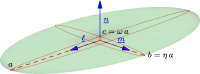
\includegraphics[width=0.7\linewidth,height=\textheight,keepaspectratio]{2_eshelby/../img/crack.pdf}

}

\caption{\label{fig-crack}Ellipsoidal crack}

\end{figure}%

In the case of cracks, it is useful to recall the second Hill
polarization tensor defined as (see (\ref{eq-defsecondHill})) \[
\uuuu{Q}=\uuuu{C}-\uuuu{C}:\uuuu{P}:\uuuu{C}
\] and in particular the so-called crack compliance
(\citeproc{ref-kachanov1992}{Kachanov, 1992}),
(\citeproc{ref-kachanov1993}{Kachanov, 1993}),
(\citeproc{ref-sevostianov2002}{Sevostianov and Kachanov, 2002}),
(\citeproc{ref-barthelemyIJES2021}{Barthélémy et al., 2021}) \[
\uuuu{H}=\lim_{\omega\to 0}\omega\,\uuuu{Q}^{-1}
\] in which it is recalled that \(\uuuu{P}\) and thus \(\uuuu{Q}\)
depend on \(\omega\) such that the components
\(\left(\uuuu{Q}^{-1}\right)_{nijk}\) (with \(n\) corresponding to the
crack normal) behave as \(1/\omega\) when \(\omega\) tends towards
\(0\). It is also shown in previously cited references that \(\uuuu{H}\)
actually derives from a symmetric second-order tensor \(\uu{B}\) as
\begin{equation}\phantomsection\label{eq-H}{
\uuuu{H}=
\lim_{\omega\to 0} \omega\,\uuuu{Q}^{-1}
=\frac{3}{4}\,\uv{n}\sotimes\uu{B}\sotimes\uv{n}
}\end{equation} For more details about this limit, the reader can also
refer to (\citeproc{ref-laws1977}{Laws, 1977}),
(\citeproc{ref-laws1985}{Laws, 1985}),
(\citeproc{ref-nemat-nasser1999}{Nemat-Nasser and Hori, 1999}),
(\citeproc{ref-barthelemyIJSS2009}{Barthélémy, 2009}),
(\citeproc{ref-kachanov2018}{Kachanov and Sevostianov, 2018}),
(\citeproc{ref-barthelemyIJES2021}{Barthélémy et al., 2021}).

For an arbitrarly anisotropic matrix, an algorithm allowing to estimate
the limit (\ref{eq-H}) is proposed in
(\citeproc{ref-barthelemyIJSS2009}{Barthélémy, 2009}) whereas in the
isotropic case \(\uu{B}\) writes \[
\uu{B}=
B_{nn}\,\uv{n}\otimes\uv{n}
+
B_{mm}\,\uv{m}\otimes\uv{m}
+
B_{\ell\ell}\,\uv{\ell}\otimes\uv{\ell}
\] with \[\begin{aligned}
B_{nn}&=\frac{8\,\eta\,(1-\nu^2)}{3\,E}\,
\frac{1}{\mathcal{E}_\eta}\label{eq:Bnn}\\
B_{mm}&=\frac{8\,\eta\,(1-\nu^2)}{3\,E}\,
\frac{1-\eta^2}{\left(1-(1-\nu)\,\eta^2\right)
\,\mathcal{E}_\eta-\nu\,\eta^2\,\mathcal{K}_\eta}\\
B_{\ell\ell}&=\frac{8\,\eta\,(1-\nu^2)}{3\,E}\,
\frac{1-\eta^2}{(1-\nu-\eta^2)\,\mathcal{E}_\eta+\nu\,\eta^2\,\mathcal{K}_\eta}
\end{aligned}\] where \(\mathcal{K}_\eta=\mathcal{K}(\sqrt{1-\eta^2})\)
and \(\mathcal{E}_\eta=\mathcal{E}(\sqrt{1-\eta^2})\) are the complete
elliptic integrals of respectively the first and second kind (see
(\citeproc{ref-abramowitz1972}{Abramowitz and Stegun, 1972})). If the
crack is circular, the components of \(\uu{B}\) become \[
B_{nn}=\frac{16\,(1-\nu^2)}{3\,\pi\,E}
\quad\textrm{;}\quad
B_{mm}=B_{\ell\ell}=\frac{B_{nn}}{1-\nu/2}
\]

\section{Numerical implementation}\label{numerical-implementation}

The syntax allowing to calculate the compliance \(\uuuu{H}\) of an
elliptical crack embedded in an infinite matrix of elastic stiffness
\(\uuuu{C}\) is very close to that corresponding to \texttt{hill} and
\texttt{eshelby} in Chapter~\ref{sec-eshelby_hill}, in other words

\texttt{H\ =\ crack\_compliance(shape,\ C,\ algo=NUMINT,\ epsroots=1.e-4,\ epsabs=1.e-4,\ epsrel=1.e-4,\ maxnb=100000)}

where the keyword argument \texttt{algo} can be either \texttt{NUMINT}
or \texttt{RESIDUES} (default: \texttt{NUMINT}). See
(\citeproc{ref-barthelemyIJSS2009}{Barthélémy, 2009}) for more details.

\begin{tcolorbox}[enhanced jigsaw, left=2mm, bottomrule=.15mm, colbacktitle=quarto-callout-warning-color!10!white, colback=white, colframe=quarto-callout-warning-color-frame, rightrule=.15mm, bottomtitle=1mm, toptitle=1mm, titlerule=0mm, title=\textcolor{quarto-callout-warning-color}{\faExclamationTriangle}\hspace{0.5em}{Warning}, toprule=.15mm, arc=.35mm, opacityback=0, opacitybacktitle=0.6, leftrule=.75mm, breakable, coltitle=black]

As recalled above the elliptical crack is described as a flat ellipsoid.
However the calculation of the crack compliance \(\uuuu{H}\)
(\ref{eq-H}) relies on an \texttt{ellipsoidal} argument (see
Section~\ref{sec-ellipsoidal}) in which even the smallest aspect ratio
should be strictly positive for numerical reasons. It is then necessary
to provide an aspect ratio \(\omega\) for the crack even if the crack
compliance is actually calculated as a limit (not depending on
\(\omega\))

\end{tcolorbox}

\textbf{Isotropic example}

\begin{Shaded}
\begin{Highlighting}[]
\NormalTok{C }\OperatorTok{=}\NormalTok{ stiff\_Enu(}\FloatTok{1.}\NormalTok{,}\FloatTok{0.2}\NormalTok{) }\OperatorTok{;} \BuiltInTok{print}\NormalTok{(}\StringTok{"C =}\CharTok{\textbackslash{}n}\StringTok{"}\NormalTok{, C)}
\NormalTok{ω }\OperatorTok{=} \FloatTok{1.e{-}4}
\NormalTok{H }\OperatorTok{=}\NormalTok{ crack\_compliance(spheroidal(ω), C) }\OperatorTok{;} \BuiltInTok{print}\NormalTok{(}\StringTok{"H =}\CharTok{\textbackslash{}n}\StringTok{"}\NormalTok{, H)}
\end{Highlighting}
\end{Shaded}

\begin{verbatim}
C =
 Order 4 ISO tensor | Param(size=2)=[ 1.66667 0.833333 ] | Angles(size=0)=[ ]
[ 1.11111 0.277778 0.277778 0 0 0 
  0.277778 1.11111 0.277778 0 0 0 
  0.277778 0.277778 1.11111 0 0 0 
  0 0 0 0.833333 0 0 
  0 0 0 0 0.833333 0 
  0 0 0 0 0 0.833333 ]

H =
 [[0.         0.         0.         0.         0.         0.        ]
 [0.         0.         0.         0.         0.         0.        ]
 [0.         0.         1.22230996 0.         0.         0.        ]
 [0.         0.         0.         0.67906109 0.         0.        ]
 [0.         0.         0.         0.         0.67906109 0.        ]
 [0.         0.         0.         0.         0.         0.        ]]
\end{verbatim}

\textbf{Anisotropic example}

\begin{Shaded}
\begin{Highlighting}[]
\NormalTok{M }\OperatorTok{=}\NormalTok{ np.array([ [}\FloatTok{2.66011}\NormalTok{, }\FloatTok{1.26432}\NormalTok{, }\FloatTok{0.662772}\NormalTok{, }\FloatTok{1.9402}\NormalTok{, }\FloatTok{1.54905}\NormalTok{, }\FloatTok{1.10384}\NormalTok{],}
\NormalTok{               [}\FloatTok{1.26432}\NormalTok{, }\FloatTok{3.6072}\NormalTok{, }\FloatTok{1.78964}\NormalTok{, }\FloatTok{2.0247}\NormalTok{, }\FloatTok{1.2701}\NormalTok{, }\FloatTok{1.1089}\NormalTok{], }
\NormalTok{               [}\FloatTok{0.662772}\NormalTok{, }\FloatTok{1.78964}\NormalTok{, }\FloatTok{2.743}\NormalTok{, }\FloatTok{1.3367}\NormalTok{, }\FloatTok{1.2962}\NormalTok{, }\FloatTok{0.897632}\NormalTok{], }
\NormalTok{               [}\FloatTok{1.9402}\NormalTok{, }\FloatTok{2.0247}\NormalTok{ ,}\FloatTok{1.3367}\NormalTok{, }\FloatTok{4.42684}\NormalTok{, }\FloatTok{2.05632}\NormalTok{, }\FloatTok{1.52686}\NormalTok{], }
\NormalTok{               [}\FloatTok{1.54905}\NormalTok{, }\FloatTok{1.2701}\NormalTok{, }\FloatTok{1.2962}\NormalTok{, }\FloatTok{2.05632}\NormalTok{, }\FloatTok{3.54431}\NormalTok{, }\FloatTok{1.3445}\NormalTok{], }
\NormalTok{               [}\FloatTok{1.10384}\NormalTok{, }\FloatTok{1.1089}\NormalTok{, }\FloatTok{0.897632}\NormalTok{, }\FloatTok{1.52686}\NormalTok{, }\FloatTok{1.3445}\NormalTok{, }\FloatTok{1.99356}\NormalTok{] ])}
\NormalTok{C }\OperatorTok{=}\NormalTok{ tensor(M) }\OperatorTok{;} \BuiltInTok{print}\NormalTok{(C)}
\NormalTok{ω }\OperatorTok{=} \FloatTok{1.e{-}4}
\NormalTok{H }\OperatorTok{=}\NormalTok{ crack\_compliance(spheroidal(ω), C, algo}\OperatorTok{=}\NormalTok{NUMINT) }\OperatorTok{;} \BuiltInTok{print}\NormalTok{(}\StringTok{"H =}\CharTok{\textbackslash{}n}\StringTok{"}\NormalTok{, H)}
\end{Highlighting}
\end{Shaded}

\begin{verbatim}
Order 4 ANISO tensor | Param(size=21)=[ 2.66011 1.26432 0.662772 1.9402 1.54905 1.10384 3.6072 1.78964 2.0247 1.2701 1.1089 2.743 1.3367 1.2962 0.897632 4.42684 2.05632 1.52686 3.54431 1.3445 1.99356 ] | Angles(size=0)=[ ]
[ 2.66011 1.26432 0.662772 1.9402 1.54905 1.10384 
  1.26432 3.6072 1.78964 2.0247 1.2701 1.1089 
  0.662772 1.78964 2.743 1.3367 1.2962 0.897632 
  1.9402 2.0247 1.3367 4.42684 2.05632 1.52686 
  1.54905 1.2701 1.2962 2.05632 3.54431 1.3445 
  1.10384 1.1089 0.897632 1.52686 1.3445 1.99356 ]

H =
 [[ 0.          0.          0.          0.          0.          0.        ]
 [ 0.          0.          0.          0.          0.          0.        ]
 [ 0.          0.          0.57167315 -0.08924584 -0.10580477  0.        ]
 [ 0.          0.         -0.08924584  0.2711102  -0.06996412  0.        ]
 [ 0.          0.         -0.10580477 -0.06996412  0.34412187  0.        ]
 [ 0.          0.          0.          0.          0.          0.        ]]
\end{verbatim}

\begin{Shaded}
\begin{Highlighting}[]
\NormalTok{H }\OperatorTok{=}\NormalTok{ crack\_compliance(spheroidal(ω), C, algo}\OperatorTok{=}\NormalTok{RESIDUES) }\OperatorTok{;} \BuiltInTok{print}\NormalTok{(}\StringTok{"H =}\CharTok{\textbackslash{}n}\StringTok{"}\NormalTok{, H)}
\end{Highlighting}
\end{Shaded}

\begin{verbatim}
H =
 [[ 0.          0.          0.          0.          0.          0.        ]
 [ 0.          0.          0.          0.          0.          0.        ]
 [ 0.          0.          0.57167315 -0.08924584 -0.10580477  0.        ]
 [ 0.          0.         -0.08924584  0.2711102  -0.06996412  0.        ]
 [ 0.          0.         -0.10580477 -0.06996412  0.34412187  0.        ]
 [ 0.          0.          0.          0.          0.          0.        ]]
\end{verbatim}

\begin{tcolorbox}[enhanced jigsaw, left=2mm, bottomrule=.15mm, colbacktitle=quarto-callout-caution-color!10!white, colback=white, colframe=quarto-callout-caution-color-frame, rightrule=.15mm, bottomtitle=1mm, toptitle=1mm, titlerule=0mm, title={Exercise}, toprule=.15mm, arc=.35mm, opacityback=0, opacitybacktitle=0.6, leftrule=.75mm, breakable, coltitle=black]

This exercise aims at checking the aspect ratio for which the
approximation
\(\omega\,\uuuu{Q}^{-1}\approx \lim_{\omega\to 0}\omega\,\uuuu{Q}^{-1}\)
remains acceptable. For this purpose it is proposed to build the graph
of relative distance between these two tensors as function of the aspect
ratio \(\omega\) for different reference stiffness tensors \(\uuuu{C}\).

\emph{Hints: with \texttt{hill\_dual} use preferably
\texttt{algo=NUMINT} and decrease the values of \texttt{epsrel} and
\texttt{espabs} to avoid roundoff error prior to inversion of
\(\uuuu{Q}\)}

\begin{Shaded}
\begin{Highlighting}[]
\NormalTok{plt.figure(figsize}\OperatorTok{=}\NormalTok{(}\DecValTok{8}\NormalTok{,}\DecValTok{3}\NormalTok{))}

\ControlFlowTok{for}\NormalTok{ i }\KeywordTok{in} \BuiltInTok{range}\NormalTok{(}\DecValTok{4}\NormalTok{):}
\NormalTok{    A }\OperatorTok{=}\NormalTok{ np.random.rand(}\DecValTok{6}\NormalTok{,}\DecValTok{6}\NormalTok{)}
\NormalTok{    C }\OperatorTok{=}\NormalTok{ tensor(A.T.dot(A) }\OperatorTok{+}\NormalTok{ np.eye(}\DecValTok{6}\NormalTok{)) }\CommentTok{\# generation of an arbitrary positive definite matrix}
\NormalTok{    ω }\OperatorTok{=} \FloatTok{1.e{-}4}
\NormalTok{    H }\OperatorTok{=}\NormalTok{ crack\_compliance(spheroidal(ω), C)}

\NormalTok{    tω }\OperatorTok{=}\NormalTok{ np.logspace(}\OperatorTok{{-}}\DecValTok{5}\NormalTok{,}\DecValTok{1}\NormalTok{,}\DecValTok{20}\NormalTok{)}
\NormalTok{    tabδ }\OperatorTok{=}\NormalTok{ []}
    \ControlFlowTok{for}\NormalTok{ ω }\KeywordTok{in}\NormalTok{ tω:}
\NormalTok{        Q }\OperatorTok{=}\NormalTok{ hill\_dual(spheroidal(ω), C, algo}\OperatorTok{=}\NormalTok{NUMINT, epsrel}\OperatorTok{=}\FloatTok{1.e{-}12}\NormalTok{, epsabs}\OperatorTok{=}\FloatTok{1.e{-}12}\NormalTok{)}
\NormalTok{        Hω }\OperatorTok{=}\NormalTok{ ω}\OperatorTok{*}\NormalTok{np.linalg.inv(Q)}
\NormalTok{        δH }\OperatorTok{=}\NormalTok{ np.linalg.norm(Hω}\OperatorTok{{-}}\NormalTok{H)}\OperatorTok{/}\NormalTok{np.linalg.norm(H)}
\NormalTok{        tabδ.append(δH)}
\NormalTok{    plt.loglog(tω,tabδ,}\StringTok{\textquotesingle{}+{-}\textquotesingle{}}\NormalTok{)}
\NormalTok{plt.xlabel(}\VerbatimStringTok{r"$\textbackslash{}omega$"}\NormalTok{)}
\NormalTok{plt.ylabel(}\VerbatimStringTok{r"$\textbackslash{}frac\{||\textbackslash{}mathbb}\SpecialCharTok{\{H\}}\VerbatimStringTok{{-}\textbackslash{}omega\textbackslash{},\textbackslash{}mathbb}\SpecialCharTok{\{Q\}}\VerbatimStringTok{\^{}\{{-}1\}||\}\{||\textbackslash{}mathbb}\SpecialCharTok{\{H\}}\VerbatimStringTok{||\}$"}\NormalTok{)}
\NormalTok{plt.grid(}\VariableTok{True}\NormalTok{,which}\OperatorTok{=}\StringTok{\textquotesingle{}both\textquotesingle{}}\NormalTok{)}
\NormalTok{plt.show()}
\end{Highlighting}
\end{Shaded}

\begin{figure}[H]

\centering{

\pandocbounded{\includegraphics[keepaspectratio]{2_eshelby/crack_compliance_files/figure-pdf/fig-errorh-output-1.pdf}}

}

\caption{\label{fig-errorh}Influence of the aspect ratio on the crack
compliance contribution tensor}

\end{figure}%

\end{tcolorbox}

\(\,\)

\bookmarksetup{startatroot}

\chapter*{References}\label{references}
\addcontentsline{toc}{chapter}{References}

\markboth{References}{References}

\phantomsection\label{refs}
\begin{CSLReferences}{1}{0}
\bibitem[\citeproctext]{ref-abramowitz1972}
Abramowitz, M., Stegun, I.A., 1972. Handbook of {Mathematical
Functions}. National Bureau of Standards - Applied Mathematics Series -
55, Washington D.C.

\bibitem[\citeproctext]{ref-echoes}
Barthélémy, J.-F., 2022. Echoes: {Extended Calculator} of
{HOmogEnization Schemes}. \url{https://doi.org/10.5281/ZENODO.10559657}

\bibitem[\citeproctext]{ref-barthelemyIJES2020_hilltrans}
Barthélémy, J.-F., 2020. Simplified approach to the derivation of the
relationship between {Hill} polarization tensors of transformed problems
and applications. International Journal of Engineering Science 154,
103326. \url{https://doi.org/10.1016/j.ijengsci.2020.103326}

\bibitem[\citeproctext]{ref-barthelemyIJSS2009}
Barthélémy, J.-F., 2009. Compliance and {Hill} polarization tensor of a
crack in an anisotropic matrix. International Journal of Solids and
Structures 46, 4064--4072.
\url{https://doi.org/10.1016/j.ijsolstr.2009.08.003}

\bibitem[\citeproctext]{ref-barthelemyIJES2021}
Barthélémy, J.-F., Sevostianov, I., Giraud, A., 2021. Micromechanical
modeling of a cracked elliptically orthotropic medium. International
Journal of Engineering Science 161, 103454.
\url{https://doi.org/10.1016/j.ijengsci.2021.103454}

\bibitem[\citeproctext]{ref-bornert2001a}
Bornert, M., Bretheau, T., Gilormini, P., 2001. Homogénéisation en
mécanique des matériaux. Hermes science.

\bibitem[\citeproctext]{ref-brisard2014a}
Brisard, S., 2014. Tensor algebra section in {Sébastien Brisard}'s blog
{[}WWW Document{]}. URL
\url{https://sbrisard.github.io/category/tensor-algebra.html}

\bibitem[\citeproctext]{ref-dormieux2006}
Dormieux, L., Kondo, D., Ulm, F.-J., 2006. Microporomechanics. John
Wiley \& Sons, Chichester, West Sussex, England ; Hoboken, NJ.
\url{https://doi.org/10.1002/0470032006}

\bibitem[\citeproctext]{ref-eshelby1957}
Eshelby, J.D., 1957. The determination of the elastic field of an
ellipsoidal inclusion, and related problems. Proceedings of the Royal
Society of London. Series A. Mathematical and Physical Sciences 241,
376--396. \url{https://doi.org/10.1098/rspa.1957.0133}

\bibitem[\citeproctext]{ref-espelid1994}
Espelid, T.O., Genz, A., 1994. {DECUHR}: An algorithm for automatic
integration of singular functions over a hyperrectangular region.
Numerical Algorithms 8, 201--220.
\url{https://doi.org/10.1007/BF02142691}

\bibitem[\citeproctext]{ref-gavazzi1990}
Gavazzi, A.C., Lagoudas, D.C., 1990. On the numerical evaluation of
{Eshelby}'s tensor and its application to elastoplastic fibrous
composites. Computational Mechanics 7, 13--19.
\url{https://doi.org/10.1007/BF00370053}

\bibitem[\citeproctext]{ref-ghahremani1977}
Ghahremani, F., 1977. Numerical evaluation of the stresses and strains
in ellipsoidal inclusions in an anisotropic elastic material. Mechanics
Research Communications 4, 89--91.
\url{https://doi.org/10.1016/0093-6413(77)90018-0}

\bibitem[\citeproctext]{ref-kachanov1993}
Kachanov, M., 1993. Elastic {Solids} with {Many Cracks} and {Related
Problems}. Advances in Applied Mechanics 30, 259--445.
\url{https://doi.org/10.1016/S0065-2156(08)70176-5}

\bibitem[\citeproctext]{ref-kachanov1992}
Kachanov, M., 1992. Effective {Elastic Properties} of {Cracked Solids}:
{Critical Review} of {Some Basic Concepts}. Applied Mechanics Reviews
45, 304--335. \url{https://doi.org/10.1115/1.3119761}

\bibitem[\citeproctext]{ref-kachanov2018}
Kachanov, M., Sevostianov, I., 2018. Micromechanics of {Materials}, with
{Applications}, Solid {Mechanics} and {Its Applications}. Springer
International Publishing, Cham.
\url{https://doi.org/10.1007/978-3-319-76204-3}

\bibitem[\citeproctext]{ref-kellogg1929}
Kellogg, O.D., 1929. Potential theory. Berlin : Springer-Verlag.

\bibitem[\citeproctext]{ref-laws1985}
Laws, N., 1985. A short note on penny-shaped cracks in transversely
isotropic materials. Mech. Mater. 4, 209--212.

\bibitem[\citeproctext]{ref-laws1977}
Laws, N., 1977. A note on interaction energies associated with cracks in
anisotropic solids. Philos. Magazine 36, 367--372.

\bibitem[\citeproctext]{ref-masson2008}
Masson, R., 2008. New explicit expressions of the {Hill} polarization
tensor for general anisotropic elastic solids. International Journal of
Solids and Structures 45, 757--769.
\url{https://doi.org/10.1016/j.ijsolstr.2007.08.035}

\bibitem[\citeproctext]{ref-milton2002}
Milton, G.W., 2002. The {Theory} of {Composites}, Cambridge {Monographs}
on {Applied} and {Computational Mathematics}. Cambridge University
Press, Cambridge. \url{https://doi.org/10.1017/CBO9780511613357}

\bibitem[\citeproctext]{ref-morin2020}
Morin, L., Gilormini, P., Derrien, K., 2020. Generalized {Euclidean
Distances} for {Elasticity Tensors}. Journal of Elasticity 138,
221--232. \url{https://doi.org/10.1007/s10659-019-09741-z}

\bibitem[\citeproctext]{ref-mura1987}
Mura, T., 1987. Micromechanics of {Defects} in {Solids}, {Second
Edition}. Kluwer Academic.
\url{https://doi.org/10.1002/zamm.19890690204}

\bibitem[\citeproctext]{ref-nemat-nasser1999}
Nemat-Nasser, S., Hori, M., 1999. Micromechanics: {Overall Properties}
of {Heterogeneous Materials} 2nd {Edition}, North Holland. ed. North
Holland, Amsterdam, The Netherlands.

\bibitem[\citeproctext]{ref-sevostianov2002}
Sevostianov, I., Kachanov, M., 2002. On elastic compliances of
irregularly shaped cracks. International Journal of Fracture 114,
245--257. \url{https://doi.org/10.1023/A:1015534127172}

\bibitem[\citeproctext]{ref-torquato2002}
Torquato, S., 2002. Random {Heterogeneous Materials}, Interdisciplinary
{Applied Mathematics}. Springer New York, New York, NY.
\url{https://doi.org/10.1007/978-1-4757-6355-3}

\bibitem[\citeproctext]{ref-walpole1984}
Walpole, L.J., 1984. Fourth-rank tensors of the thirty-two crystal
classes: Multiplication tables. Proceedings of the Royal Society of
London. A. Mathematical and Physical Sciences 391, 149--179.
\url{https://doi.org/10.1098/rspa.1984.0008}

\bibitem[\citeproctext]{ref-willis1977}
Willis, J.R., 1977. Bounds and self-consistent estimates for the overall
properties of anisotropic composites. Journal of the Mechanics and
Physics of Solids 25, 185--202.
\url{https://doi.org/10.1016/0022-5096(77)90022-9}

\bibitem[\citeproctext]{ref-withers1989}
Withers, P.J., 1989. The determination of the elastic field of an
ellipsoidal inclusion in a transversely isotropic medium, and its
relevance to composite materials. Philosophical Magazine A 59, 759--781.
\url{https://doi.org/10.1080/01418618908209819}

\end{CSLReferences}

\(\,\)

\cleardoublepage
\phantomsection
\addcontentsline{toc}{part}{Appendices}
\appendix

\chapter{Tensor algebra}\label{sec-tensor_algebra}

\section{Conventions of tensor
algebra}\label{sec-tensoralgebra_convention}

This appendix presents some conventions regarding tensor algebra in the
usual three-dimensional euclidean space \(E=\R^3\). In the sequel,
tensor components are associated to an orthonormal frame
\((\ve{i})_{i=1,2,3}\) so that introducing the notion of tensor variance
is useless here. The following presentation relies on the prior
knowledge of the definition of tensors as multilinear operators and the
classical isomorphism between the euclidean space and its dual through
the scalar product
\begin{equation}\phantomsection\label{eq-scalarprod}{\begin{aligned}
\phi\,\colon E & \longrightarrow  E^* \\
       \uv{v} & \longmapsto \uv{v}\cdot\bullet
\end{aligned}}\end{equation} which allows to identify vectors and linear
forms.

Consider two tensors \(\mathcal{T}\) and \(\mathcal{T}'\) of respective
orders \(p\) and \(q\). The tensor product
\(\mathcal{T}\otimes\mathcal{T}'\) is the \((p+q)\) order tensor
decomposed as \begin{equation}\phantomsection\label{eq-otimes}{
\mathcal{T}\otimes\mathcal{T}'=\mathcal{T}_{i_1,\ldots,i_p} \,\mathcal{T}'_{i_{p+1},\ldots,i_{p+q}}\,
\ve{i_1}\otimes\ldots\otimes\ve{i_{p+q}}
}\end{equation} where Einstein convention of immplicit summation over
repeated indices is adopted and
\(\ve{i_1}\otimes\ldots\otimes\ve{i_{p+q}}\) is the multilinear form
such that\footnote{\(\delta_{ij}=1\) if \(i=j\) and \(0\) if \(i\neq j\)
  (Kronecker symbol)} \begin{equation}\phantomsection\label{eq-multfom}{
(\ve{i_1}\otimes\ldots\otimes\ve{i_{p+q}})(\ve{j_1},\ldots,\ve{j_{p+q}})
=
\delta_{i_1,j_1}\ldots \delta_{i_{p+q},j_{p+q}}
}\end{equation} The notation \(\mathcal{T}\sotimes\mathcal{T}'\)
indicates a tensor product followed by a symmetrization over the last
index of \(\mathcal{T}\) and the first of \(\mathcal{T}'\), i.e.
\begin{equation}\phantomsection\label{eq-sotimes}{
\mathcal{T}\sotimes\mathcal{T}'=
\frac{\mathcal{T}_{i_1,\ldots,i_p} \,\mathcal{T}'_{i_{p+1},\ldots,i_{p+q}}
+
\mathcal{T}_{i_1,\ldots,i_{p+1}} \,\mathcal{T}'_{i_p,\ldots,i_{p+q}}
}{2}
\,\ve{i_1}\otimes\ldots\otimes\ve{i_{p+q}}
}\end{equation} It follows that
\begin{equation}\phantomsection\label{eq-sotimesuv}{
\uv{u}\sotimes\uv{v}=\frac{\uv{u}\otimes\uv{v}+\uv{v}\otimes\uv{u}}{2}
}\end{equation} and an example of generalization involving a
second-order tensor \(\uu{a}\) and vectors \(\uv{u}\) and \(\uv{v}\)
\begin{equation}\phantomsection\label{eq-sotimesuav}{
\uv{u}\sotimes\uu{a}\sotimes\uv{v}=
\frac{u_i\,a_{jk}\,v_l+u_i\,a_{jl}\,v_k+u_j\,a_{ik}\,v_l+u_j\,a_{il}\,v_k}{4}
\,\ve{i}\otimes\ve{j}\otimes\ve{k}\otimes\ve{l}
}\end{equation}

The simple dot product or contracted product between \(\mathcal{T}\) and
\(\mathcal{T}'\) involves by convention a contraction between the last
index of \(\mathcal{T}\) and the first of \(\mathcal{T}'\), which leads
to the \((p+q-2)\) order tensor
\begin{equation}\phantomsection\label{eq-simpledot}{
\mathcal{T}\cdot\mathcal{T}'=\mathcal{T}_{i_1,\ldots,i_{p-1},{\color{red}k}} \,\mathcal{T}'_{{\color{red}k},i_{p},\ldots,i_{p+q-2}}\,
\ve{i_1}\otimes\ldots\otimes\ve{i_{p+q-2}}
}\end{equation}

As regards the double dot product, the classical convention consists in
consuming the indices going up from the extremities, which means that a
first contraction acts as in the simple dot product then a second
contraction is performed between the penultimate index of
\(\mathcal{T}\) and the second one of \(\mathcal{T}'\). However and
alternate convention adopted here is proposed in
(\citeproc{ref-brisard2014a}{Brisard, 2014})\footnote{see
  \url{https://sbrisard.github.io/posts/20140219-on_the_double_dot_product.html}},
which somehow consists in considering that the double contraction
operates over the two last indices of \(\mathcal{T}\) as a pair and the
two first indices of \(\mathcal{T}'\) as the corresponding pair. In
other words, this operation is such that if \(\uu{a}\) and \(\uu{b}\)
are two second-order tensors and \(\uuuu{T}\) is a fourth-order tensor
\begin{equation}\phantomsection\label{eq-doubledot}{
\uu{a}:\uu{b}=a_{ij}b_{ij}
\quad\textrm{and}\quad
\uuuu{T}:\uu{a}=T_{ijkl}\, a_{kl}\, \ve{i}\otimes\ve{j}
}\end{equation} and the transpose tensor \(\trans{\uuuu{T}}\) is
consistently defined by
\begin{equation}\phantomsection\label{eq-trans4}{
\trans{\uuuu{T}}:\uu{a}=\uu{a}:\uuuu{T}
\quad\Leftrightarrow\quad
\left(\trans{\uuuu{T}}\right)_{ijkl}=\left(\uuuu{T}\right)_{klij}
}\end{equation} The quadruple dot product is introduced as a scalar
product between fourth-order tensors as
\begin{equation}\phantomsection\label{eq-dot4}{
\uuuu{T}:\uuuu{T}'=T_{ijkl} T'_{ijkl}
}\end{equation}

Another useful operator introduced in
(\citeproc{ref-brisard2014a}{Brisard, 2014})\footnote{see
  \url{https://sbrisard.github.io/posts/20140226-decomposition_of_transverse_isotropic_fourth-rank_tensors.html}}
is the modified tensor product denoted by \(\boxtimes\). The
fourth-order tensor \(\uu{a}\boxtimes\uu{b}\) (where \(\uu{a}\) and
\(\uu{b}\) are two second-order tensors) is defined by its operation
over any second-order tensor \(\uu{p}\) and by its components
\begin{equation}\phantomsection\label{eq-boxtimes}{\begin{aligned}
& (\uu{a}\boxtimes\uu{b}):\uu{p}=\uu{a}\cdot\uu{p}\cdot\trans{\uu{b}}
=a_{ik}\,p_{kl}\,b_{jl}\,\ve{i}\otimes\ve{j}
\\
& \left(\uu{a}\boxtimes\uu{b}\right)_{ijkl}=a_{ik}\,b_{jl}
\end{aligned}}\end{equation}

A symmetrized version of \(\boxtimes\) denoted by \(\sboxtimes\) can
also be introduced. It operates as
\begin{equation}\phantomsection\label{eq-sboxtimes}{\begin{aligned}
& (\uu{a}\sboxtimes\uu{b}):\uu{p}=
(\uu{a}\boxtimes\uu{b}):\left(\frac{\uu{p}+\trans{\uu{p}}}{2}\right)
=\uu{a}\cdot\left(\frac{\uu{p}+\trans{\uu{p}}}{2}\right)\cdot\trans{\uu{b}}
\\
& (\uu{a}\sboxtimes\uu{b})_{ijkl}=\frac{a_{ik}\,b_{jl}+a_{il}\,b_{jk}}{2}
\end{aligned}}\end{equation}

It follows from these definitions that the fourth-order identity, as an
operator over second-order tensors, writes
\(\uuuu{1}=\uu{1}\boxtimes\uu{1}\) where \(\uu{1}\) is the second-order
identity. The fourth-order operator allowing to extract the symmetric
part of a second-order tensor writes
\(\uuuu{I}=\uu{1}\sboxtimes\uu{1}\). The latter tensor, which obviously
complies with the conditions of minor symmetries, is classically used to
play the role of fourth-order identity operating over symmetric
second-order tensors.

Some remarkable relationships result from the previous definitions
\begin{equation}\phantomsection\label{eq-propboxtimes}{\begin{aligned}
&(\uu{a}\boxtimes\uu{b}):(\uv{u}\otimes\uv{v})=
(\uu{a}\cdot\uv{u})\otimes(\uu{b}\cdot\uv{v})
&(a) \\
&(\uu{a}\boxtimes\uu{b}):(\uu{c}\boxtimes\uu{d})=
(\uu{a}\cdot\uu{c})\boxtimes(\uu{b}\cdot\uu{d})
&(b) \\
&(\uu{a}\sboxtimes\uu{b}):(\uu{c}\sboxtimes\uu{d})=
\frac{(\uu{a}\cdot\uu{c})\sboxtimes(\uu{b}\cdot\uu{d})+
(\uu{a}\cdot\uu{d})\sboxtimes(\uu{b}\cdot\uu{c})}{2}
&(c) \\
&(\uu{a}\sboxtimes\uu{a}):(\uu{b}\sboxtimes\uu{b})=
(\uu{a}\cdot\uu{b})\sboxtimes(\uu{a}\cdot\uu{b})
&(d) \\
&\trans{(\uu{a}\boxtimes\uu{b})}=\trans{\uu{a}}\boxtimes\trans{\uu{b}}
&(e) \\
&\trans{(\uu{a}\sboxtimes\uu{a})}=\trans{\uu{a}}\sboxtimes\trans{\uu{a}}
\;\textrm{ but }\;
\trans{(\uu{a}\sboxtimes\uu{b})}\neq\trans{\uu{a}}\sboxtimes\trans{\uu{b}}
&(f) \\
&(\uu{a}\boxtimes\uu{b})^{-1}=\uu{a}^{-1}\boxtimes\uu{b}^{-1}
&(g) \\
&(\uu{a}\sboxtimes\uu{a})^{-1}:\uu{p}=(\uu{a}^{-1}\sboxtimes\uu{a}^{-1}):\uu{p}
\;\textrm{ if }\;\trans{\uu{p}}=\uu{p}
\;\textrm{ but }\;
(\uu{a}\sboxtimes\uu{b})^{-1}\neq\uu{a}^{-1}\sboxtimes\uu{b}^{-1}
&(h)
\end{aligned}}\end{equation}

\section{Kelvin-Mandel notation}\label{sec-KM}

The Kelvin-Mandel notation allows to write the matrix of a symmetric
second-order tensor in a given orthonormal frame
\mbox{$(\ve{i})_{i=1,2,3}$} under the form of a vector of \(\R^6\)
\begin{equation}\phantomsection\label{eq-KM2}{
   \Mat(\eps,(\ve{i}))=
   \left(
   \begin{array}{ccc}
   \varepsilon_{11} & \varepsilon_{12} & \varepsilon_{31}\\
   \varepsilon_{12} & \varepsilon_{22} & \varepsilon_{23}\\
   \varepsilon_{31} & \varepsilon_{23} & \varepsilon_{33}
   \end{array}
   \right)
   \mapsto
   \left(
   \begin{array}{c}
   \varepsilon_{11} \\
   \varepsilon_{22} \\
   \varepsilon_{33} \\
   \sqrt{2}\,\varepsilon_{23} \\
   \sqrt{2}\,\varepsilon_{31} \\
   \sqrt{2}\,\varepsilon_{12}
   \end{array}
   \right)
}\end{equation}

The vector of \(\R^6\) in (\ref{eq-KM2}) corresponds to the components
of the second-order tensor \(\eps\) in the basis ordered as
\begin{equation}\phantomsection\label{eq-basisKM}{
\mathcal{B}=\left(
\ve{1}\otimes\ve{1},
\ve{2}\otimes\ve{2},
\ve{3}\otimes\ve{3},
\sqrt{2}\,\ve{2}\otimes\ve{3},
\sqrt{2}\,\ve{3}\otimes\ve{1},
\sqrt{2}\,\ve{1}\otimes\ve{2}
\right)
}\end{equation}

The tensors of the basis (\ref{eq-basisKM}) form an orthonormal frame
spanning the space of symmetric second-order tensors equipped with the
double contraction ``\(:\)'' as scalar product. It follows that the
double contraction between symmetric second-order tensors is no other
than the classical scalar product of the corresponding vectors of
\(\R^6\) written according to the convention (\ref{eq-KM2}).

\begin{tcolorbox}[enhanced jigsaw, left=2mm, bottomrule=.15mm, colbacktitle=quarto-callout-note-color!10!white, colback=white, colframe=quarto-callout-note-color-frame, rightrule=.15mm, bottomtitle=1mm, toptitle=1mm, titlerule=0mm, title=\textcolor{quarto-callout-note-color}{\faInfo}\hspace{0.5em}{Note}, toprule=.15mm, arc=.35mm, opacityback=0, opacitybacktitle=0.6, leftrule=.75mm, breakable, coltitle=black]

Note the effect of \(\sqrt{2}\) on the off-diagonal components. Unlike
\href{https://en.wikipedia.org/wiki/Voigt_notation}{Voigt convention},
the choice of Kelvin-Mandel convention throughout all the library allows
to address strain and stress tensors under the same synthetic
representation.

\end{tcolorbox}

A fourth-order tensor with minor symetries
(\(C_{jikl}=C_{ijlk}=C_{ijkl}\)), which can be seen as a linear operator
acting over symmetric second-order tensors by double contraction, writes
in the same convention under the form of a \(6\times 6\) square matrix
(the solid lines separate blocks affected by different factors whereas
the colored components highlight a central block playing a major role in
the sequel) \begin{equation}\phantomsection\label{eq-KM4}{
\small
\Mat(\uuuu{C},\mathcal{B})=
   \left(
   \begin{array}{ccc|ccc}
   C_{1111} & C_{1122} & C_{1133} & \sqrt{2}\,C_{1123} & \sqrt{2}\,C_{1131} & \sqrt{2}\,C_{1112} \\
   C_{2211} & C_{2222} & C_{2233} & \sqrt{2}\,C_{2223} & \sqrt{2}\,C_{2231} & \sqrt{2}\,C_{2212} \\
   C_{3311} & C_{3322} & \color{red}C_{3333} & \color{red}\sqrt{2}\,C_{3323} & \color{red}\sqrt{2}\,C_{3331} & \sqrt{2}\,C_{3312} \\
   \hline
   \sqrt{2}\,C_{2311} & \sqrt{2}\,C_{2322} & \color{red}\sqrt{2}\,C_{2333} & \color{red}2\,C_{2323} & \color{red}2\,C_{2331} & 2\,C_{2312} \\
   \sqrt{2}\,C_{3111} & \sqrt{2}\,C_{3122} & \color{red}\sqrt{2}\,C_{3133} & \color{red}2\,C_{3123} & \color{red}2\,C_{3131} & 2\,C_{3112} \\
   \sqrt{2}\,C_{1211} & \sqrt{2}\,C_{1222} & \sqrt{2}\,C_{1233} & 2\,C_{1223} & 2\,C_{1231} & 2\,C_{1212}
   \end{array}
   \right)
}\end{equation} The result of \(\uuuu{C}:\eps\) writes as a classical
matrix-vector product of (\ref{eq-KM4}) by (\ref{eq-KM2}).

However another way of ordering the tensors of (\ref{eq-basisKM}) which
proves useful for the calculation of crack compliance is based on a
gathering of one set of three in-plane and another one of three
out-of-plane tensors (the latter involving \(\n=\ve{3}\) assumed to be
the normal of the crack and the former not)
\begin{equation}\phantomsection\label{eq-basisKM2}{
\mathcal{B}^*=\Bigg(
\underbrace{
\ve{1}\otimes\ve{1},
\ve{2}\otimes\ve{2},
\sqrt{2}\,\ve{1}\sotimes\ve{2}
}_{\textrm{in-plane}},
\quad
\underbrace{
\ve{3}\otimes\ve{3},
\sqrt{2}\,\ve{2}\sotimes\ve{3},
\sqrt{2}\,\ve{3}\sotimes\ve{1}
}_{\textrm{out-of-plane}}
\Bigg)
}\end{equation} such that the matrix of \(\uuuu{C}\) in
\(\mathcal{B}^*\) is now obtained by permutations of lines and columns
of (\ref{eq-KM4}) to give
\begin{equation}\phantomsection\label{eq-KM4bis}{
\small
\Mat(\uuuu{C},\mathcal{B}^*)=
   \left(
   \begin{array}{ccc|ccc}
   C_{1111} & C_{1122} & \sqrt{2}\,C_{1112} & C_{1133} & \sqrt{2}\,C_{1123} & \sqrt{2}\,C_{1131} \\
   C_{2211} & C_{2222} & \sqrt{2}\,C_{2212} & C_{2233} & \sqrt{2}\,C_{2223} & \sqrt{2}\,C_{2231} \\
   \sqrt{2}\,C_{1211} & \sqrt{2}\,C_{1222} & 2\,C_{1212} & \sqrt{2}\,C_{1233} & 2\,C_{1223} & 2\,C_{1231} \\
   \hline
   C_{3311} & C_{3322} & \sqrt{2}\,C_{3312} & C_{3333} & \sqrt{2}\,C_{3323} & \sqrt{2}\,C_{3331} \\
   \sqrt{2}\,C_{2311} & \sqrt{2}\,C_{2322} & 2\,C_{2312} & \sqrt{2}\,C_{2333} & 2\,C_{2323} & 2\,C_{2331} \\
   \sqrt{2}\,C_{3111} & \sqrt{2}\,C_{3122} & 2\,C_{3112} & \sqrt{2}\,C_{3133} & 2\,C_{3123} & 2\,C_{3131}
   \end{array}
   \right)
}\end{equation} One may notice that the bottom right \(3\times 3\) block
of (\ref{eq-KM4bis}) exactly corresponds to the colored block in
(\ref{eq-KM4}).

\section{Rotation of tensors}\label{sec-rottens}

Recalling that the set of second-order tensors is isomorphic to the set
of endomorphisms in an euclidean space, it is natural to define a
rotation tensor as an element of the special orthogonal group,
i.e.~tensors \(\uu{R}\) such that \(\trans{\uu{R}}\cdot\uu{R}=\uu{1}\)
and \(\det{\uu{R}}=1\). In \(\R^3\) equipped with an orthonormal frame
\((\ve{i})_{i=1,2,3}\), these tensors can be defined by three Euler
angles \((θ,ϕ,ψ)∈[0,π]×[0,2π]×[0,2π]\) (see Fig.~\ref{fig-eulerangles})
such that\footnote{with the simplifying writing convention
  \(c_\theta=\cos\theta\), \(s_\theta=\sin\theta\), \(c_\phi=\cos\phi\),
  \(s_\phi=\sin\phi\), \(c_\psi=\cos\psi\), \(s_\psi=\sin\psi\)}
\begin{equation}\phantomsection\label{eq-rot3}{
\small
\Mat(\uu{R},(\ve{i}))=
   \left(
   \begin{array}{ccc}
   c_\theta  c_\psi  c_\phi - s_\psi  s_\phi & - c_\theta  c_\phi  s_\psi - c_\psi  s_\phi & c_\phi  s_\theta \\
   c_\theta  c_\psi  s_\phi + c_\phi  s_\psi & - c_\theta  s_\psi  s_\phi + c_\psi  c_\phi & s_\theta  s_\phi \\
   - c_\psi  s_\theta & s_\theta  s_\psi & c_\theta \\
   \end{array}
   \right) 
}\end{equation} A rotated frame \((\underline{e}'_i)_{i=1,2,3}\) is
obtained by application of the rotation \(\uu{R}\) on the vectors
\(\ve{i}\) (see Fig.~\ref{fig-eulerangles})
\begin{equation}\phantomsection\label{eq-Rei}{
\forall i \in \{1,2,3\}\quad \underline{e}'_i=\uu{R}\cdot\ve{i}
}\end{equation}

\begin{figure}

\centering{

\includegraphics[width=0.4\linewidth,height=\textheight,keepaspectratio]{99_appendices/../img/sphcoor.pdf}

}

\caption{\label{fig-eulerangles}Euler angles}

\end{figure}%

The rotation of Eurler angles \((\theta,\phi,\psi)\) applies on a \(p\)
order tensor \(\mathcal{T}\) as
\begin{equation}\phantomsection\label{eq-rotT}{
\mathcal{T}=
\mathcal{T}_{i_1,\ldots,i_p} \,\ve{i_1}\otimes\ldots\otimes\ve{i_{p}}
\overset{\uu{R}}{\longmapsto}
\uu{R}(\mathcal{T})=
\mathcal{T}_{i_1,\ldots,i_p} \,(\uu{R}\cdot\ve{i_1})\otimes\ldots\otimes(\uu{R}\cdot\ve{i_{p}})
}\end{equation}

The application of (\ref{eq-rotT}) to a second-order tensor \(\uu{a}\)
therefore gives \begin{equation}\phantomsection\label{eq-rotT2}{
\uu{R}(\uu{a})=\uu{R}\cdot 
\uu{a}
\cdot\trans{\uu{R}}
}\end{equation} and to a fourth-order tensor \(\uuuu{T}\)
\begin{equation}\phantomsection\label{eq-rotT4}{
\uu{R}(\uuuu{T})=(\uu{R}\sboxtimes\uu{R}):
\uuuu{T}
:\trans{(\uu{R}\sboxtimes\uu{R})}
}\end{equation} where the fourth-order rotation tensor
\(\uuuu{R}=\uu{R}\sboxtimes\uu{R}\) can be expressed in Kelvin-Mandel
notation (\ref{eq-KM4}) by means of the components of \(\uu{R}\) defined
in (\ref{eq-rot3}) \begin{equation}\phantomsection\label{eq-rot6}{
\scriptsize
\Mat(\uuuu{R},\mathcal{B})=
   \left(
\begin{array}{cccccc}
R_{1 1}^{2} & R_{1 2}^{2} & R_{1 3}^{2} & \sqrt{2}  R_{1 2}  R_{1 3} & \sqrt{2}  R_{1 1}  R_{1 3} & \sqrt{2}  R_{1 1}  R_{1 2} \\
R_{2 1}^{2} & R_{2 2}^{2} & R_{2 3}^{2} & \sqrt{2}  R_{2 2}  R_{2 3} & \sqrt{2}  R_{2 1}  R_{2 3} & \sqrt{2}  R_{2 1}  R_{2 2} \\
R_{3 1}^{2} & R_{3 2}^{2} & R_{3 3}^{2} & \sqrt{2}  R_{3 2}  R_{3 3} & \sqrt{2}  R_{3 1}  R_{3 3} & \sqrt{2}  R_{3 1}  R_{3 2} \\
\sqrt{2}  R_{2 1}  R_{3 1} & \sqrt{2}  R_{2 2}  R_{3 2} & \sqrt{2}  R_{2 3}  R_{3 3} & R_{2 2}  R_{3 3} + R_{2 3}  R_{3 2} & R_{2 1}  R_{3 3} + R_{2 3}  R_{3 1} & R_{2 1}  R_{3 2} + R_{2 2}  R_{3 1} \\
\sqrt{2}  R_{1 1}  R_{3 1} & \sqrt{2}  R_{1 2}  R_{3 2} & \sqrt{2}  R_{1 3}  R_{3 3} & R_{1 2}  R_{3 3} + R_{1 3}  R_{3 2} & R_{1 1}  R_{3 3} + R_{1 3}  R_{3 1} & R_{1 1}  R_{3 2} + R_{1 2}  R_{3 1} \\
\sqrt{2}  R_{1 1}  R_{2 1} & \sqrt{2}  R_{1 2}  R_{2 2} & \sqrt{2}  R_{1 3}  R_{2 3} & R_{1 2}  R_{2 3} + R_{1 3}  R_{2 2} & R_{1 1}  R_{2 3} + R_{1 3}  R_{2 1} & R_{1 1}  R_{2 2} + R_{1 2}  R_{2 1} \\
\end{array}
\right)
}\end{equation} It results that (\ref{eq-rotT4}) can be seen as a
classical rotation operation involving matrix multiplications in
\(\R^6\).

\section{Fourth-order isotropic tensors}\label{sec-ISO}

This paragraph concerns fourth-order tensors operating over symmetrical
second-order tensors, which allows to impose that they satisfy the minor
symmetries (\(C_{jikl}=C_{ijlk}=C_{ijkl}\)). The identity operator is
given by \begin{equation}\phantomsection\label{eq-tensI}{
\uuuu{I}=\uu{1}\sboxtimes\uu{1}=
\frac{\delta_{ik}\delta_{jl}+\delta_{il}\delta_{jk}}{2}\,\ve{i}\otimes\ve{j}\otimes\ve{k}\otimes\ve{l}
}\end{equation} of identity matrix in Kelvin-Mandel convention
\begin{equation}\phantomsection\label{eq-matI}{
\small
\Mat(\uuuu{I},\mathcal{B})=
   \left(
   \begin{array}{ccc|ccc}
   1 & 0 & 0 & 0 & 0 & 0 \\
   0 & 1 & 0 & 0 & 0 & 0 \\
   0 & 0 & 1 & 0 & 0 & 0 \\
   \hline
   0 & 0 & 0 & 1 & 0 & 0 \\
   0 & 0 & 0 & 0 & 1 & 0 \\
   0 & 0 & 0 & 0 & 0 & 1 \\
   \end{array}
   \right)
}\end{equation}

It is classically proven that any minor-symmetrical fourth-order tensor
invariant by rotation (\ref{eq-rotT4}) write as a linear combination on
the two projectors \(\uuuu{J}\) and \(\uuuu{K}\) which respectively
extract the spherical and deviatoric part of any symmetrical
second-order tensor \begin{equation}\phantomsection\label{eq-JKext}{
\uuuu{J}:\uu{a}=\frac{1}{3}\tr{\uu{a}}\,\uu{1}
\quad \textrm{and} \quad
\uuuu{K}:\uu{a}=\uu{a}-\frac{1}{3}\tr{\uu{a}}\,\uu{1}
}\end{equation} In other words, \(\uuuu{J}\) and \(\uuuu{K}\) are
defined by \begin{equation}\phantomsection\label{eq-JK}{
\uuuu{J}=\frac{1}{3}\uu{1}\otimes\uu{1}
\quad \textrm{and} \quad
\uuuu{K}=\uuuu{I}-\uuuu{J}=\uu{1}\sboxtimes\uu{1}-\frac{1}{3}\uu{1}\otimes\uu{1}
}\end{equation} their components by
\begin{equation}\phantomsection\label{eq-JKijkl}{
J_{ijkl}=\frac{1}{3}\delta_{ij}\delta_{ik}
\quad \textrm{and} \quad
K_{ijkl}=\frac{\delta_{ik}\delta_{jl}+\delta_{il}\delta_{jk}}{2}-\frac{1}{3}\delta_{ij}\delta_{ik}
}\end{equation} and their matrices in Kelvin-Mandel notation relatively
to any orthonormal frame by
\begin{equation}\phantomsection\label{eq-matJ}{
\small
\Mat(\uuuu{J},\mathcal{B})=
   \left(
   \begin{array}{ccc|ccc}
   \frac{1}{3} & \frac{1}{3} & \frac{1}{3} & 0 & 0 & 0 \\
   \frac{1}{3} & \frac{1}{3} & \frac{1}{3} & 0 & 0 & 0 \\
   \frac{1}{3} & \frac{1}{3} & \frac{1}{3} & 0 & 0 & 0 \\
   \hline
   0 & 0 & 0 & 0 & 0 & 0 \\
   0 & 0 & 0 & 0 & 0 & 0 \\
   0 & 0 & 0 & 0 & 0 & 0 \\
   \end{array}
   \right)
}\end{equation}

\begin{equation}\phantomsection\label{eq-matK}{
\small
\Mat(\uuuu{K},\mathcal{B})=
   \left(
   \begin{array}{ccc|ccc}
   \frac{2}{3} & \frac{-1}{3} & \frac{-1}{3} & 0 & 0 & 0 \\
   \frac{-1}{3} & \frac{2}{3} & \frac{-1}{3} & 0 & 0 & 0 \\
   \frac{-1}{3} & \frac{-1}{3} & \frac{2}{3} & 0 & 0 & 0 \\
   \hline
   0 & 0 & 0 & 1 & 0 & 0 \\
   0 & 0 & 0 & 0 & 1 & 0 \\
   0 & 0 & 0 & 0 & 0 & 1 \\
   \end{array}
   \right)
}\end{equation}

The following relationships are easily obtained
\begin{equation}\phantomsection\label{eq-relJK}{
\uuuu{J}:\uuuu{J}=\uuuu{J}
\quad ; \quad
\uuuu{K}:\uuuu{K}=\uuuu{K}
\quad ; \quad
\uuuu{J}:\uuuu{K}=\uuuu{0}
\quad ; \quad
\uuuu{J}::\uuuu{J}=1
\quad ; \quad
\uuuu{K}::\uuuu{K}=5
}\end{equation}

The isotropisation of any fourth-order tensor \(\uuuu{T}\) is defined by
(\citeproc{ref-bornert2001a}{Bornert et al., 2001})
\begin{equation}\phantomsection\label{eq-isoT}{
\ISO(\uuuu{T})=\left(\uuuu{T}::\uuuu{J}\right)\,\uuuu{J}+\left(\frac{\uuuu{T}::\uuuu{K}}{5}\right)\,\uuuu{K}
}\end{equation} It is easy to show that (\ref{eq-isoT}) is no other than
the closest isotropic tensor to \(\uuuu{T}\) if the distance is chosen
as the euclidean one i.e.~associated to the scalar product
(\ref{eq-dot4}). Note however that this isotropisation relying on
euclidean distance to the set of isotropic tensors does not lead to the
same result if \(\uuuu{T}'\) is considered instead of \(\uuuu{T}\).
Other distance definitions such as log-Euclidean distance fullfilling
invariance by inversion are analyzed in (\citeproc{ref-morin2020}{Morin
et al., 2020}).

\section{Fourth-order transversely isotropic tensors and Walpole
basis}\label{sec-TI}

The Walpole basis ((\citeproc{ref-walpole1984}{Walpole, 1984}),
(\citeproc{ref-brisard2014a}{Brisard, 2014})\footnote{see
  \url{https://sbrisard.github.io/posts/20140226-decomposition_of_transverse_isotropic_fourth-rank_tensors.html}})
allowing to write any fourth-order transversely isotropic relatively to
a an axis oriented by the unit vector \(\n\) is composed of the six
following tensors built from \(\uu{1}_n=\n\otimes\n\) and
\(\uu{1}_T=\uu{1}-\uu{1}_n\)
\begin{equation}\phantomsection\label{eq-WalpoleBasis}{\begin{aligned}
& \uuuu{W}_1=\uu{1}_n\otimes\uu{1}_n
\quad\textrm{ ; }\quad
\uuuu{W}_2=\frac{\uu{1}_T\otimes\uu{1}_T}{2}
&\textrm{ ; }&
\uuuu{W}_3=\frac{\uu{1}_n\otimes\uu{1}_T}{\sqrt{2}}
\quad\textrm{ ; }\quad
\uuuu{W}_4=\frac{\uu{1}_T\otimes\uu{1}_n}{\sqrt{2}}
&(a) \\
& \uuuu{W}_5=\uu{1}_T\sboxtimes\uu{1}_T-\frac{\uu{1}_T\otimes\uu{1}_T}{2}
&\textrm{ ; }&
\uuuu{W}_6=\uu{1}_T\sboxtimes\uu{1}_n+\uu{1}_n\sboxtimes\uu{1}_T
&(b)
\end{aligned}}\end{equation}

Any transversely isotropic fourth-order tensor can be decomposed as
\begin{equation}\phantomsection\label{eq-decWalpole}{
{\uuuu{L}} = {\ell}_{1}\,{\uuuu{E}}_{1} + {\ell}_{2}\,{\uuuu{E}}_{2} +
{\ell}_{3}\,{\uuuu{E}}_{3}+ {\ell}_{4}\,{\uuuu{E}}_{4}+ {\ell}_{5}\,{\uuuu{E}}_{5}+
{\ell}_{6}\,{\uuuu{E}}_{6}
}\end{equation}

The six parameters can be conveniently gathered in a triplet composed of
a \(2 \times 2\) matrix containing the four first parameters \(\ell_i\)
(\(1\leq i \leq 4\)) and the two last parameters \(\ell_5\) and
\(\ell_6\) \begin{equation}\phantomsection\label{eq-syntWalpole}{
\uuuu{L} \equiv \left( L , {\ell}_{5} , {\ell}_{6}
\right) , \quad
L = \left(
      \begin{array}{cc}
        {\ell}_{1} & {\ell}_{3} \\
        {\ell}_{4} & {\ell}_{2} \\
      \end{array}
    \right)
}\end{equation}

Such a synthetic notation allows simple calculations of products and
inverses which consist in classical matrix or scalar products and
inverses
\begin{equation}\phantomsection\label{eq-calWalpole}{\begin{aligned}
& \uuuu{L} : \uuuu{M} \equiv \left( L M , {\ell}_{5} m_5 , {\ell}_{6} m_6
\right)
&(a) \\
& {\uuuu{L}}^{-1} \equiv \left( {L}^{-1} , \frac{1}{{\ell}_{5}} , \frac{1}{{\ell}_{6}}
\right)
&(b)
\end{aligned}}\end{equation}

A symmetrized version of the Walpole also exists; it is composed of the
following tensors

\begin{equation}\phantomsection\label{eq-symWalpoleBasis}{\begin{aligned}
& \uuuu{W}^s_1=\uu{1}_n\otimes\uu{1}_n
\quad\textrm{ ; }\quad
\uuuu{W}^s_2=\frac{\uu{1}_T\otimes\uu{1}_T}{2}
&\textrm{ ; }&
\uuuu{W}^s_3=\frac{\uu{1}_n\otimes\uu{1}_T}{\sqrt{2}}+\frac{\uu{1}_T\otimes\uu{1}_n}{\sqrt{2}}
&(a) \\
& \uuuu{W}^s_4=\uu{1}_T\sboxtimes\uu{1}_T-\frac{\uu{1}_T\otimes\uu{1}_T}{2}
&\textrm{ ; }&
\uuuu{W}^s_5=\uu{1}_T\sboxtimes\uu{1}_n+\uu{1}_n\sboxtimes\uu{1}_T
&(b)
\end{aligned}}\end{equation}

\chapter{Hill polarization tensors}\label{sec-hill_elas}

This section recalls some results about the calculation of the Hill
polarization tensors related to a matrix of stiffness \(\mathbb{C}\) and
an ellipsoid \(\mathcal{E}_{\uu{A}}\) of equation \[
\uv{x}\in\mathcal{E}_{\uu{A}}
\quad\Leftrightarrow\quad
\uv{x}\cdot(\trans{\uu{A}}\cdot\uu{A})^{-1}\cdot\uv{x}\leq 1
\] where \(\uu{A}\) is an invertible second-order tensor so that
\(\trans{\uu{A}}\cdot\uu{A}\) is a positive definite symmetric tensor
associated to 3 radii (eigenvalues \(a\geq b \geq c\) possibly written
\(\rho_1 \geq \rho_2 \geq \rho_3\) for convenience) and 3 angles
(orientation of the frame of eigenvectors
\(\uv{e}_1, \uv{e}_2, \uv{e}_3\))
\begin{equation}\phantomsection\label{eq-ellipsoid}{
\trans{\uu{A}}\cdot\uu{A}=a^2 \uv{e}_1\otimes\uv{e}_1 + b^2 \uv{e}_2\otimes\uv{e}_2 + c^2 \uv{e}_3\otimes\uv{e}_3 = \sum_{i=1}^3 \rho_i \uv{e}_i\otimes\uv{e}_i
}\end{equation}

\section{\texorpdfstring{\(a>b>c\)
(ellipsoid)}{a\textgreater b\textgreater c (ellipsoid)}}

\begin{longtable}[]{@{}
  >{\centering\arraybackslash}p{(\linewidth - 2\tabcolsep) * \real{0.5000}}
  >{\centering\arraybackslash}p{(\linewidth - 2\tabcolsep) * \real{0.5000}}@{}}
\toprule\noalign{}
\begin{minipage}[b]{\linewidth}\centering
\(I_i\)
\end{minipage} & \begin{minipage}[b]{\linewidth}\centering
\textbf{Value}
\end{minipage} \\
\midrule\noalign{}
\endfirsthead
\toprule\noalign{}
\begin{minipage}[b]{\linewidth}\centering
\(I_i\)
\end{minipage} & \begin{minipage}[b]{\linewidth}\centering
\textbf{Value}
\end{minipage} \\
\midrule\noalign{}
\endhead
\bottomrule\noalign{}
\tabularnewline
\caption{\(I_i\) for ellipsoid with arbitrary
radii}\label{tbl-Ii}\tabularnewline
\endlastfoot
\(I_1\) &
\(\frac{a\,b\,c}{(a^2-b^2)\sqrt{a^2-c^2}}\,\left({\cal F}-{\cal E}\right)\) \\
\(I_2\) & \(1-I_1-I_3\) \\
\(I_3\) &
\(\frac{a\,b\,c}{(b^2-c^2)\sqrt{a^2-c^2}}\,\left(\frac{b\sqrt{a^2-c^2}}{a\,c}-{\cal E}\right)\) \\
\end{longtable}

\section{\texorpdfstring{\(a>b=c\)
(prolate)}{a\textgreater b=c (prolate)}}

\begin{longtable}[]{@{}
  >{\centering\arraybackslash}p{(\linewidth - 2\tabcolsep) * \real{0.5000}}
  >{\centering\arraybackslash}p{(\linewidth - 2\tabcolsep) * \real{0.5000}}@{}}
\toprule\noalign{}
\begin{minipage}[b]{\linewidth}\centering
\(I_i\)
\end{minipage} & \begin{minipage}[b]{\linewidth}\centering
\textbf{Value}
\end{minipage} \\
\midrule\noalign{}
\endfirsthead
\toprule\noalign{}
\begin{minipage}[b]{\linewidth}\centering
\(I_i\)
\end{minipage} & \begin{minipage}[b]{\linewidth}\centering
\textbf{Value}
\end{minipage} \\
\midrule\noalign{}
\endhead
\bottomrule\noalign{}
\tabularnewline
\caption{\(I_i\) for prolate spheroid}\label{tbl-Iipro}\tabularnewline
\endlastfoot
\(I_1\) & \(1-2\,I_3\) \\
\(I_2\) & \(I_3\) \\
\(I_3\) &
\(a\,\frac{a\sqrt{a^2-c^2}-c^2\,\arcosh{(a/c)}}{2\left(a^2-c^2\right)^{3/2}}\) \\
\end{longtable}

\section{Elasticity}\label{elasticity}

\subsection{General expression}\label{general-expression}

A general expression of the elastic polarization tensor is derived in
(\citeproc{ref-willis1977}{Willis, 1977}) (see also
(\citeproc{ref-mura1987}{Mura, 1987}))
\begin{equation}\phantomsection\label{eq-Hill}{\begin{aligned}
\uuuu{P}(\uu{A},\uuuu{C})&=\frac{1}{4\pi}
\int_{\norm{\uv{\zeta}}=1}
(\uu{A}^{-1}\cdot\uv{\zeta})\sotimes
\Big((\uu{A}^{-1}\cdot\uv{\zeta})\cdot\uuuu{C}
\cdot(\uu{A}^{-1}\cdot\uv{\zeta})\Big)^{-1}
\sotimes(\uu{A}^{-1}\cdot\uv{\zeta})
\ud S_\zeta\\
&=
\frac{\det{\uu{A}}}{4\pi}
\int_{\norm{\uv{\xi}}=1}
\frac{\uv{\xi}\sotimes
(\uv{\xi}\cdot\uuuu{C}
\cdot\uv{\xi})^{-1}
\sotimes\uv{\xi}}{\norm{\uu{A}\cdot\uv{\xi}}^3}
\ud S_{\xi}
\end{aligned}}\end{equation}

When \(\uuuu{C}\) is arbitrarily anisotropic, it is necessary to resort
to numerical cubature to estimate \(\uuuu{P}\) as proposed in
(\citeproc{ref-ghahremani1977}{Ghahremani, 1977}),
(\citeproc{ref-gavazzi1990}{Gavazzi and Lagoudas, 1990}) or
(\citeproc{ref-masson2008}{Masson, 2008}). However in some cases of
anisotropy, analytical solutions are available
((\citeproc{ref-withers1989}{Withers, 1989}),
(\citeproc{ref-barthelemyIJES2020_hilltrans}{Barthélémy, 2020})). The
case of isotropic matrix is particularly developed in the next section.

\subsection{Isotropic matrix}\label{isotropic-matrix}

In this section, the matrix is assumed isotropic so that its stiffness
tensor writes by means of a bulk \(k\) and shear \(\mu\) or Lamé
\(\lambda\) and \(\mu\) moduli or even Young modulus \(E\) and Poisson
ratio \(\nu\) with \(k=\frac{E}{3(1-2\nu)}\) and
\(\mu=\frac{E}{2(1+\nu)}\).
\begin{equation}\phantomsection\label{eq-isoC}{\begin{aligned}
\uuuu{C} =& {} 3k\uuuu{J}+2\mu\uuuu{K} =  3\lambda\uuuu{I}+2\mu\uuuu{K}\\
 & \quad\textrm{with}\quad J_{ijkl}=\frac{\delta_{ij}\delta_{kl}}{3},
I_{ijkl}=\frac{\delta_{ik}\delta_{jl}+\delta_{il}\delta_{jk}}{2}
\textrm{ and }
\uuuu{K}=\uuuu{I}-\uuuu{J}
\end{aligned}}\end{equation}

Introducing (\ref{eq-isoC}) in (\ref{eq-Hill}) leads to after some
algebra \[
\uuuu{P}=
\frac{1}{\lambda+2\,\mu}
\uuuu{U}
+\frac{1}{\mu}(\uuuu{V}-\uuuu{U})
\] where the tensors \(\uuuu{U}\) and \(\uuuu{V}\), depending only on
the ellipsoidal tensor \(\uu{A}\) of (\ref{eq-ellipsoid}), are given by
(see (\citeproc{ref-barthelemyIJES2020_hilltrans}{Barthélémy, 2020}))
\[\begin{aligned}
\uuuu{U} &= \frac{\det{\uu{A}}}{4\pi}
\int_{\norm{\uv{\xi}}=1}
\frac{\uv{\xi}\otimes\uv{\xi}\otimes\uv{\xi}\otimes\uv{\xi}}
{\norm{\uu{A}\cdot\uv{\xi}}^3}\ud S_{\xi}\\
&=
\frac{1}{4\pi}
\int_{\norm{\uv{\zeta}}=1}
\frac{%
(\uu{A}^{-1}\cdot\uv{\zeta})
\otimes
(\uu{A}^{-1}\cdot\uv{\zeta})
\otimes
(\uu{A}^{-1}\cdot\uv{\zeta})
\otimes
(\uu{A}^{-1}\cdot\uv{\zeta})
}{\norm{\uu{A}^{-1}\cdot\uv{\zeta}}^4}
\ud S_{\zeta}
\end{aligned}\] and \[\begin{aligned}
\uuuu{V} &= \frac{\det{\uu{A}}}{4\pi}
\int_{\norm{\uv{\xi}}=1}
\frac{\uv{\xi}\sotimes\uu{1}\sotimes\uv{\xi}}
{\norm{\uu{A}\cdot\uv{\xi}}^3}\ud S_{\xi}\\
&=
\frac{1}{4\pi}
\int_{\norm{\uv{\zeta}}=1}
\frac{%
(\uu{A}^{-1}\cdot\uv{\zeta})
\sotimes
\uu{1}
\sotimes
(\uu{A}^{-1}\cdot\uv{\zeta})
}{\norm{\uu{A}^{-1}\cdot\uv{\zeta}}^2}
\ud S_{\zeta}
\end{aligned}\] For an arbitrary ellipsoid defined by
(\ref{eq-ellipsoid}), the components of \(\uuuu{U}\) and \(\uuuu{V}\)
write \[\begin{aligned}
U_{iiii}&=\frac{3(I_i-\rho_i^2I_{ii})}{2} 
\quad\forall\, i\in\{1,2,3\}\\
U_{iijj}=U_{ijij}=U_{ijji}&=\frac{I_j-\rho_i^2I_{ij}}{2} 
=\frac{I_i-\rho_j^2I_{ij}}{2}
\quad\forall\, i\neq j\in\{1,2,3\}
\end{aligned}\] and \[\begin{aligned}
V_{iiii}&=I_i\quad\forall\, i\in\{1,2,3\}\\
V_{ijij}=V_{ijji}&=\frac{I_i+I_j}{4}
\quad\forall\, i\neq j\in\{1,2,3\}
\end{aligned}\] where the coefficients \(I_i\) and \(I_{ij}\) are given
by (note that \(I_i\) and \(I_{ij}\) are adapted from those provided in
(\citeproc{ref-kellogg1929}{Kellogg, 1929}) and
(\citeproc{ref-eshelby1957}{Eshelby, 1957}): they differ by a factor of
\(4\pi/3\) for \(I_{ij}\) with \(i\neq j\) and by \(4\pi\) for the
others)

\begin{itemize}
\tightlist
\item
  if \(a > b > c\) \[\begin{aligned}
    I_1&=\frac{a\,b\,c}{(a^2-b^2)\sqrt{a^2-c^2}}\,
    \left({\cal F}-{\cal E}\right)\\
    I_3&=\frac{a\,b\,c}{(b^2-c^2)\sqrt{a^2-c^2}}\,
    \left(\frac{b\sqrt{a^2-c^2}}{a\,c}-
    {\cal E}\right)\\
    I_2&=1-I_1-I_3\\
    I_{ij}&=\frac{I_j-I_i}{\rho_i^2-\rho_j^2}\quad\forall\, i\neq j\in\{1,2,3\}\\
    I_{ii}&=\frac{1}{3}\left(
    \frac{1}{\rho_i^2}-
    \sum_{j\neq i}I_{ij} \right) 
    \quad\forall\, i\in\{1,2,3\}
    \end{aligned}\]\\
  where \({\cal F}={\cal F}(\theta,\kappa)\) and
  \({\cal E}={\cal E}(\theta,\kappa)\) are respectively the elliptic
  integrals of the first and second kinds (see
  (\citeproc{ref-abramowitz1972}{Abramowitz and Stegun, 1972})) of
  amplitude and parameter \[
    \theta=\arcsin{\sqrt{1-\frac{c^2}{a^2}}}
    \quad;\quad
    \kappa=\sqrt{\frac{a^2-b^2}{a^2-c^2}}
    \]
\item
  if \(a > b = c\) (prolate spheroid) \[\begin{aligned}
    I_2=I_3&=a\,
    \frac{a\sqrt{a^2-c^2}-c^2\,\arcosh{(a/c)}}
    {2\left(a^2-c^2\right)^{3/2}}\\
    I_1&=1-2\,I_3\\
    I_{1i}=I_{i1}&=\frac{I_i-I_1}{a^2-\rho_i^2}\quad
    \forall\, i\in\{2,3\}\\
    I_{ij}&=\frac{1}{4}
    \left(\frac{1}{c^2}-I_{31} \right) 
    \quad\forall\, i,j\in\{2,3\}\\
    I_{11}&=\frac{1}{3}
    \left(\frac{1}{a^2}-2\,I_{31} \right)
    \end{aligned}\]
\item
  if \(a = b > c\) (oblate spheroid) \[\begin{aligned}
    I_1=I_2&=c\,
    \frac{a^2\,\arccos{(c/a)}-c\sqrt{a^2-c^2}}
    {2\left(a^2-c^2\right)^{3/2}}\\
    I_3&=1-2\,I_1\\
    I_{3i}=I_{i3}&=\frac{I_3-I_i}{\rho_i^2-c^2}\quad
    \forall\, i\in\{1,2\}\\
    I_{ij}&=\frac{1}{4}
    \left(\frac{1}{a^2}-I_{31} \right) 
    \quad\forall\, i,j\in\{1,2\}\\
    I_{33}&=\frac{1}{3}
    \left(\frac{1}{c^2}-2\,I_{31} \right)
    \end{aligned}\]
\item
  if \(a = b = c\) (sphere) \[\begin{aligned}
    I_1=I_2=I_3&=\frac{1}{3}\\
    I_{ij}&=\frac{1}{5\,a^2}\quad\forall\, i,j\in\{1,2,3\}
    \end{aligned}\]
\end{itemize}

In this last case of spherical inclusion (\(\uu{A}=\uu{1}\)),
\(\uuuu{U}\) and \(\uuuu{V}\) are simply decomposed as \[
\uuuu{U}=\frac{1}{3}\uuuu{J}+\frac{2}{15}\uuuu{K}
\quad\textrm{ and }\quad
\uuuu{V}=\frac{1}{3}\uuuu{I}
\]

\chapter{Basic problem of elasticity
homogenization}\label{sec-basics_elas}

\section{System of equations}\label{sec-basics_elas_sys_eq}

Consider a representative volume element (RVE) \(\Omega\) composed of a
heterogeneous material. Neglecting body forces in a problem posed at the
scale of a RVE is consistent with the fact that the order of magnitude
of mechanical effects induced by body forces is in general much lower
than that of the macroscopic strain \(\E\) or stress \(\Sig\) effects
accounting for interactions with particles surrounding the RVE (see
(\citeproc{ref-dormieux2006}{Dormieux et al., 2006})). The hypothesis of
quasi-static equilibrium is also invoked here to write the balance law
involving the Cauchy stress field \(\sig\)
\begin{equation}\phantomsection\label{eq-divsigma}{
\divu{\sig}=\uv{0} \quad(\Omega)
}\end{equation}

In the sequel, the small perturbation hypothesis is adopted so that the
strain field \(\eps\) derives from the displacement one \(\uv{u}\) as
the symmetrical part of its gradient
\begin{equation}\phantomsection\label{eq-epsgradu}{
\eps=\frac{\graduu{\uv{u}}+\trans{\graduu{\uv{u}}}}{2} \quad(\Omega)
}\end{equation}

In the framework of random media homogenization, two types of conditions
applied at the boundary \(\partial\Omega\) of a RVE \(\Omega\) are
usually considered:

\begin{itemize}
\item
  \emph{homogeneous strain boundary conditions} corresponding to
  prescribed displacements \(\uv{u}^g\) at \(\partial\Omega\)
  \begin{equation}\phantomsection\label{eq-homstrainBC}{
  \uv{u}^g=\E\cdot\x \quad(\partial\Omega)
  }\end{equation} It is noticeable that in this case the divergence
  theorem implies the following relationship between the microscopic and
  macroscopic strain tensors
  \begin{equation}\phantomsection\label{eq-EhomstrainBC}{
  <\eps>_{\Omega}=\frac{1}{\lvert \Omega \rvert}\int_\Omega \eps\ud \Omega
  =\frac{1}{\lvert \Omega \rvert}\int_{\partial\Omega} \uv{u}\sotimes\n \ud S
  =\E
  }\end{equation} where the spatial average over a domain \(\omega\) is
  denoted by \(<\bullet>_\omega\) and \(\n\) is the unit outward normal
  at the boundary. The macroscopic stress tensor is then simply defined
  as the average \begin{equation}\phantomsection\label{eq-ShomstrainBC}{
  \Sig=
  <\sig>_{\Omega}=\frac{1}{\lvert \Omega \rvert}\int_\Omega \sig\ud \Omega
  }\end{equation}
\item
  \emph{homogeneous stress boundary conditions} corresponding to
  prescribed surface tractions \(\uv{T}^g\) at \(\partial\Omega\)
  \begin{equation}\phantomsection\label{eq-homstressBC}{
  \uv{T}^g=\Sig\cdot\n \quad(\partial\Omega)
  }\end{equation} Now owing to the remarkable identity
  \((x_i\sigma_{jk})_{,k}=\sigma_{ij}\) resulting from
  (\ref{eq-divsigma}) and the symmetry of \(\sig\), the relationship
  between the microscopic and macroscopic stress is ensured by the
  divergence theorem
  \begin{equation}\phantomsection\label{eq-ShomstressBC}{
  <\sig>_{\Omega}=\frac{1}{\lvert \Omega \rvert}\int_\Omega \sig\ud \Omega
  =\frac{1}{\lvert \Omega \rvert}\int_{\partial\Omega} \x\sotimes(\sig\cdot\n) \ud S
  =\Sig
  }\end{equation} The macroscopic stress tensor is then simply defined
  as the average \begin{equation}\phantomsection\label{eq-EhomstressBC}{
  \E=
  <\eps>_{\Omega}=\frac{1}{\lvert \Omega \rvert}\int_\Omega \eps\ud \Omega
  }\end{equation}
\end{itemize}

\begin{tcolorbox}[enhanced jigsaw, left=2mm, bottomrule=.15mm, colbacktitle=quarto-callout-note-color!10!white, colback=white, colframe=quarto-callout-note-color-frame, rightrule=.15mm, bottomtitle=1mm, toptitle=1mm, titlerule=0mm, title=\textcolor{quarto-callout-note-color}{\faInfo}\hspace{0.5em}{Hill lemma}, toprule=.15mm, arc=.35mm, opacityback=0, opacitybacktitle=0.6, leftrule=.75mm, breakable, coltitle=black]

Note that whatever the choice of boundary conditions between
(\ref{eq-homstrainBC}) and (\ref{eq-homstressBC}), the consistency
between the microscopic and macroscopic works is ensured by
\begin{equation}\phantomsection\label{eq-Hilllemma}{
<\sig:\eps>_{\Omega}
=\frac{1}{\lvert \Omega \rvert}\int_\Omega \sig:\eps\ud \Omega
=\frac{1}{\lvert \Omega \rvert}\int_{\partial\Omega} \uv{u}\cdot\sig\cdot\n \ud S
=\Sig:\E
}\end{equation} which results from the application of the divergence
theorem to
\((u_i\sigma_{ij})_{,k}=u_{i,j}\sigma_{ij}=\varepsilon_{ij}\sigma_{ij}\).

\end{tcolorbox}

The set of equations defining the problem posed on the RVE is finally
completed by the local constitutive law relating the strain and stress
fields. The hypothesis of linear elasticity is adopted in this part so
that \begin{equation}\phantomsection\label{eq-Hooke}{
\sig=\uuuu{c}:\eps \quad(\Omega)
}\end{equation} where \(\uuuu{c}(\x)\) denotes the heterogeneous
(positive definite fourth-order) stiffness tensor field satisfying the
conditions of minor (\(c_{jikl}=c_{ijlk}=c_{ijkl}\)) and major
(\(c_{klij}=c_{ijkl}\)) symmetries. The compliance tensor field is
introduced as the inverse \(\uuuu{s}=\uuuu{c}^{-1}\) in the sense of
fourth-order tensors operating over symmetrical second-order tensors.

In short, the system of equations posed on the RVE is given by
(\ref{eq-divsigma}), (\ref{eq-epsgradu}), (\ref{eq-homstrainBC}) or
(\ref{eq-homstressBC}) and (\ref{eq-Hooke}).

\section{Macroscopic stiffness or compliance
tensors}\label{sec-basics_elas_mac_stiff}

Whatever the boundary condition of homogeneous strain or stress type
(\ref{eq-homstrainBC}) or (\ref{eq-homstressBC}), the linearity of the
problem allows to invoke the existence of concentration tensors relating
the microscopic strain \(\eps\) and stress \(\sig\) fields to the
macroscopic strain \(\E\) or stress \(\Sig\) tensors
\begin{equation}\phantomsection\label{eq-conc}{\begin{aligned}
\eps & =  \uuuu{A}_E:\E \\
\sig & =  \uuuu{B}_E:\E \quad\textrm{with}\quad \uuuu{B}_E=\uuuu{c}:\uuuu{A}_E \\
\sig & =  \uuuu{B}_\Sigma:\Sig \\
\eps & =  \uuuu{A}_\Sigma:\Sig \quad\textrm{with}\quad \uuuu{A}_\Sigma=\uuuu{s}:\uuuu{B}_\Sigma 
\end{aligned}}\end{equation}




\end{document}
